\documentclass{report}

%----- Packages to be imported
\usepackage{physics}
\usepackage{amsmath}
\usepackage{amssymb}
\usepackage{epsfig}
\usepackage{setspace}
\usepackage{fancyhdr}
\usepackage{graphicx}
\usepackage{color}
\usepackage{chemformula}
\usepackage{tablefootnote}
\usepackage{threeparttable}
%\usepackage{subfigure}
\usepackage{float}
\usepackage{gensymb}
\usepackage{siunitx}
\usepackage{booktabs}
%\usepackage[superscript]{cite}

%----captions subfigure caption packages---%
\usepackage{caption}
\usepackage[noabbrev]{cleveref}
\usepackage{subfig}
\captionsetup[subfigure]{subrefformat=simple,labelformat=simple,listofformat=subsimple}
\renewcommand\thesubfigure{(\alph{subfigure})}
%------------------------------------------%

\usepackage[toc,page]{appendix}
\usepackage[left=2.5cm,top=3cm,right=2.5cm,bottom=3cm,bindingoffset=0.5cm]{geometry}
\usepackage[printonlyused]{acronym}

%\usepackage[superscript,biblabel]{cite} uncomment for superscript in-text
%	citations

\usepackage[nottoc,notlof,notlot]{tocbibind}
\renewcommand\bibname{References}

\usepackage{macros/macros_custom}

\def\Nile{{\sc Nile}}
%\includeonly{file_list with commas as delimiters, no spaces}  %this option allows only selected range of filesto be included in the output, but all other files are taken into account for page numbering references etc.
\includeonly{frontmatter/title,chapters/results}

\pagestyle{plain}

\begin{document}

\setcounter{secnumdepth}{4}
	%\sets numbering upto 4th level in chapter,section, subsection, subsubsection
\setcounter{tocdepth}{4}
	%\makes levels upto the 4th appear in the table of contents

%---- Roman page numbering for frontmatter
	\pagenumbering{roman}
	\setcounter{page}{1}
\thispagestyle{empty}
\begin{titlepage}

	\begin{center}

	\singlespacing
	\textbf{TITLE}\\
	\doublespacing
	
	by\\
	
	\textbf{Kraig Andrews}\\
	Ph.D. Disseration Prospectus\\ 

	\end{center}

\end{titlepage} %!!!!!!!!!!!!!uncomment
	\begin{center}
\textbf{ABSTRACT}
	
	
	\singlespacing
\textbf{Quantum Transport Properties and Scattering Mechanisms in Transition Metal Dichalcogenides}\\
	\doublespacing
	
	by\\
	
	\textbf{Kraig J. Andrews}\\
	February 2016\\
\end{center}
\begin{tabular}{ll}	
Advisor: & Dr. Zhixain Zhou\\
Major:   &Physics\\
Degree:  &Doctor of Philosophy
\end{tabular}
\bigskip

\noindent Two-dimensional materials have garnered much interest since the isolation of graphene. Since then layered materials, such as transition metal dichalcogenides (TMDs) have been studied extensively. However, several key problems have yet to be solved. In this study we propose using methods developed to decrease and minimize contact resistance through a novel approach of 2D/2D contacts and \hbn encapsulation to study how the mobility and intrinsic properties are affect by $p$-doping \ch{WSe2} device channels. Preliminary results show contact resistance as low as $0.185\unita{k\Omega\cdot\mu m}$ using degenerately doped contacts and field-effect mobilities of $\sim 200\cmvs$ and $\sim 650\cmvs$ at $T=300\unita{K}$ and $T=5{K}$, respectively using this 2D/2D contact \hbn encapsulation method. In addition, this method is intended to improve mobility at both room temperature for device applications and at low temperatures ($\sim 4\unita{K}$) to study the integer quantum hall effect (IQHE) and the corresponding related quantum oscillations (Shubnikov-de Haas oscillations) to determine information related to quantum scattering times, effective cyclotron mass, and the geometry of the Fermi surface. 
 %!!!!!!!!!!!!!uncomment

	\renewcommand{\contentsname}{Table of Contents}
        \tableofcontents
	\newpage
        \addcontentsline{toc}{section}{List of Figures}
	\listoffigures 
	\newpage
	\addcontentsline{toc}{section}{List of Tables}
	\listoftables
	\newpage
	\pagenumbering{arabic}
         \pagestyle{fancy}
        \fancyhead{} 
	\fancyfoot{} % clear all header and footer fields
        \chead[]{\thepage}
        \renewcommand{\headrulewidth}{0pt}
         \renewcommand{\footrulewidth}{0pt}
	%\pagestyle{myheadings}%supposed to put pg number in header
	%\pagenumbering{arabic}
	\fancypagestyle{plain}{%
	\fancyhf{} % clear all header and footer fields
	\fancyhead[C]{\thepage} % except the center
	\renewcommand{\headrulewidth}{0pt}
	\renewcommand{\footrulewidth}{0pt}}

%---- End of front matter
	\pagenumbering{arabic}
	\chapter{Introduction}\label{sec:intro}
\section{Early Semiconductors}\label{sec:early_semicond}
The development of microelectronics revolutionized the world in the latter half of the twentieth century. The term semiconductor, in the sense it is known today, first appears in literature in 1911 \cite{Koenigsberger_AnnalenDerPhysik1911}. Initially, work on the subject was rather pessimistic. However, in the years following Word War II breakthroughs began shed light on the possible applications and the underlying physics involved, such as the ideas of \emph{instrinsic} and \emph{extrinsic} semiconductors \cite{Busch_EuroJournPhys1989,Lark_AAAS1954,Wilson_Royal1931a,Wilson_Royal1931b}. \\

%\noindent
The history of semiconductors and transistors is a well documented subject. The first transistor was constructed at Bell Labs in 1947 using polycrystalline germanium. Shortly thereafter one was developed using silicon. Throughout the following years, these devices were improved on by replacing polycrystalline with single crystals \cite{Neamen_Semiconductor_Physics2003}. Then Jack Kilby demonstrated the first  \ac{IC} in 1958, for which he would win the Nobel Prize in physics \cite{Lukasiak_JorunTelcomm2010, Kilby_Patent1959}. The scale of \acp{IC} grew rapidly in the subsequent years. Initially only a few transistors could fit on a chip (small-scale integration), in stark contrast to modern-day chips that contains billions of transistors \cite{Moore_Electronics1965, Clarke_EEtimes2005}. Growth continued at a rapid pace, but eventually it was realized that some limits, material and integration based, existed in silicon and other commonly used materials \cite{Meindl_Science2001, Schulz_Nature1999}. In part, these limitations increased the interest in alternative materials. As a result widespread and renewed interest has led to a breadth information and results on a wide range of materials and their applications.

\section{Graphene as a New \Td Material}\label{sec:graphene}
Layered materials have existed for a long time, and have been studied over the last few centuries \cite{Golden_EarthSci2013,Brodie_Royal1859}. In recent decades the scientific study of graphite (3D) has led to new forms of materials, such as carbon nanotubes (1D) and fullerenes (0D) \cite{Kroto_Nature1985, Balleste_Nanoscale2011,Iijima_Nature1991}. However, only more recently have scientists began to understand the potential of such layered materials and their potential technological applications. After attempting unsuccessfully to synthesize few-layer graphite during the 1960s, only around 10-50 layers were able to be synthesized, a breakthrough was finally acheived \cite{Balleste_Nanoscale2011}. This most notably began with the synthesis of monolayer graphene \cite{Novoselov_Science2004}.

\subsection{Properties of Graphene}\label{subsec:graphene_properties}
To date, graphene's properties have been the focus of much research, both theoretical and experimental. It has been one of the primary driving forces in study of `relativistic' condensed matter physics due to its low dimensionality and its band structure that allows electrons to mimic relativistic particles confirming the appearance of several relativistic phonomena \cite{Geim_NatureMat2007,Geim_Nature2005,Zhang_NatPhys2011,Williams_Science2007}. In its most basic sense, graphene is composed of a single layer of carbon atoms arranged in \td honeycomb lattice (see fig.~\subref*{fig:graphene_honeycomb}) It has a Young's modulus of $~100\unita{GPa}$ (several times more than steel) with a breaking force that is $13\%$ of its Young's modulus \cite{Bertolazzi_ACSnano2011, Akinwande_NatureComm2014}. Its stength is due, in part, to its strong in-plane carbon (\ch{C}) bonds. In addition, graphene can sustain elastic deformations of 20\% due to its \td nature and it has high pliability \cite{Balleste_Nanoscale2011}. These mechanical properties are of interest because graphene lies in the extreme ranges of many metrics considering its size and dimensionality.\\

%\noindent 
Aside from its mechanical properties, graphene's transport properties were another reason why the material was so appealing. Graphene's mobility is several times that of silicon's (electron mobility $\mu\sim 1400\cmvs$, hole mobility $\mu\sim 450\cmvs$ at room temperature). Experimental results have shown graphene mobility around $15,000\cmvs$ with a potential theoretical limit of $200,000\cmvs$ \cite{Dargys_Encylco1994,Akinwande_NatureComm2014,Si_Properties}. The upper theoretical limit imposed on mobility is due to scattering, however, these high mobilities are achieved mainly because electrons in graphene act very much like photons in their mobility due to their lack of mass. This enables them to travel sub-micron distances without scattering \cite{Novoselov_NatureMat2007}. In reality, there are other limiting factors that need to be considered such as the quality of graphene and scattering with the substrate, for example. 
\begin{figure}[ht]
	\centering
	\subfloat[]{
		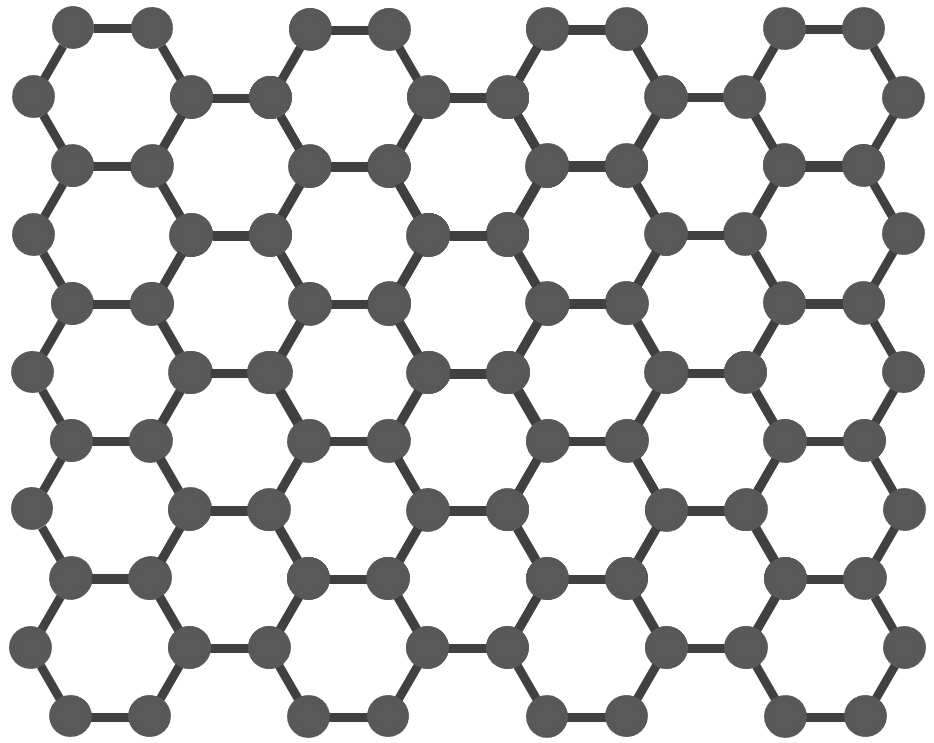
\includegraphics[height=4cm,width=5cm]{figs/intro/graphene_honeycomb}
		\label{fig:graphene_honeycomb}
	}
	\qquad
	\subfloat[]{
		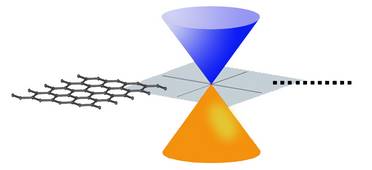
\includegraphics[height=4cm,width=6cm]{figs/intro/graphene_bandgap}
		\label{fig:graphene_bandgap}
	}
	\caption[Lattice and band structure of graphene]{\protect\subref{fig:graphene_honeycomb} Graphene: a layer of carbon atoms in a honeycomb lattice. \protect\subref{fig:graphene_bandgap} One of the most unusual features of graphene is that its conduction and valence bands meet at a point, meaning that in single-layer graphene there is no bandgap (Figures obtained from \cite{Berkley_Online2009}).}
	\label{fig:graphene_structures}
\end{figure}

\subsection{Band Structure of Graphene}\label{subsec:graphene_bandstructure}
%\noindent 
Despite its impressive properties, the main drawback of graphene is its lack of bandgap. As this became known, the prospect of using graphene for the fabrication to \acp{IC} became unlikely. In graphene the conduction and valence bands touch at a single point as shown in fig.~\subref*{fig:graphene_bandgap} \cite{Wallace_PhysRev1947}. Ultimately, the lack of a bandgap means that the current on/off ratio is low and is unappealing for logical circuit applications \cite{Xu_ChemRev2013}. However, graphene exhibits some interesting properties as a result of having no bandgap, particularly as it pertains to its optical properties. The material's band structure allows for absorption of light over a large range of the electromagnetic spectrum, ranging from infrared ($<1.65\unita{eV}$) to ultraviolet ($>3.2\unita{eV}$), offering potential electronic-photonic device applications \cite{Xia_NatureNano2009,Wang_Science2008,Geim_NatureComm2011}. Since a direct use in logical circuits is not practical researchers have moved on to look for `\td materials beyond graphene.' Several attempts at some derivatives of graphene-like materials have been studied, but for the most part they do not seem promising for use in logical circuits \cite{Takeda_PhysRev1994,Cahangirov_PhysRevLett2009}. As of late, research has been concentrated on \td materials, namely transition methal dichalcogenides, as a candidate in \acp{IC} and other potential device applications.

\section{\Td Materials: Transition Metal Dichalcogenides}\label{sec:tmds}
Commonly referred to \td materials beyond graphene, transition metal dichalcogenides (TMDs) have garnered much interest in recent years. \acp{TMD} were studied previously, however, they have gained renewed interest due to their properties \cite{Frindt_Royal1963,Fivaz_PhysRev1967,Mattheiss_PhysRevB1973,Wilson_AdvPhys1969}. \acp{TMD} consist of hexagonal layers of metal (\ch{M}) atoms in between two layers of chalcogen (\ch{X}) atoms (see fig.~\subref*{fig:tmd_hexagonal}), such that the stoichiometry of the material is \ch{MX2} \cite{Xu_ChemRev2013}. The material is dependent on the type of transition metal, typically one of: \ac{Mo}, \ac{W}, \ac{Nb}, \ac{Re}, \ac{Ni}, or \ac{V}, and two chalcogen atoms, typically one of: \ac{S}, \ac{Se}, or \ac{Te} \cite{Wilson_AdvPhys1969,Wells_Oxford1984}. The most commonly studied variations of \acp{TMD} are \ac{MoS2}, \ac{WSe2}, and \ac{WS2}. These materials are commonly stacked together involving van der Waals interactions between adjacent sheets and covalent bonding within each individual sheet (see fig.~\subref*{fig:tmd_layer}) \cite{Xu_ChemRev2013}.
\begin{figure}[ht]
	\centering
	\subfloat[]{
		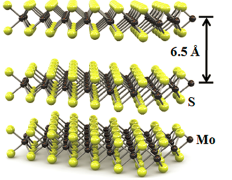
\includegraphics[height=4cm,width=6cm]{figs/intro/tmdlayered}
		\label{fig:tmd_layer}
	}
	\qquad
	\subfloat[]{
		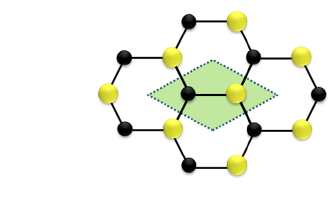
\includegraphics[height=4cm,width=6cm]{figs/intro/tmdhexagonal}
		\label{fig:tmd_hexagonal}
	}
	\caption[Hexagonal lattice structure of \acs{TMD}]{\protect\subref{fig:tmd_layer} The atomic structure of a layered \acs{TMD}, depicting \acs{MoS2}. Each sheet is composed of three atoms with \ch{Mo} sandwiched in between two \acs{S} atoms, \acs{S}-\acs{Mo}-\acs{S}. \protect\subref{fig:tmd_hexagonal} Top view of a \acs{TMD} (\acs{MoS2}) lattice. (Figures obtained from \cite{Kis_NatureNano2011})}
\end{figure}
%\noindent 
\acp{TMD} have been found to exhibit a wide variety of interesting properties, including either being a metal or insulator, and displaying the topological insulator effect, superconductivity, and thermoelectricity \cite{Lang_ACSnano2012,Zhang_AdvMat2012,Xie_AppPhysLett2009,Gamble_JournChemPhys1975}.

\subsection{Band Structures of \acp{TMD}}\label{subsec:tmd_properties}
%\noindent
\noindent As stated in sec.~\ref{subsec:graphene_bandstructure}, one important propert as it pertains to applications for logical circuits is the material's band structure. One of the main reasons \acp{TMD} have been so extensively studied lately is due to the fact that, unlike graphene, they do exhibit a bandgap. The bandgaps in some commonly used \acp{TMD} is interesting because of the transition from an indirect to a direct bandgap as the layered thickness decreases. Fig.~\ref{fig:mos2_bandstructure} illustrates this, for bulk and few-layer \acs{MoS2} there is an indirect band gap while for monolayer \acs{MoS2} there is a direct bandgap. This unusual structure results in some unique optical properties making monolayer \acs{TMD} promising candidates for optoelectronic devices \cite{Cheng_NanoLett2014,Conley_NanoLett2013}. Table~\ref{table:band_gaps} summarizes some \acs{TMD} bandgap energies that are of considerable interest to the device fabrication process. 
\begin{figure}[ht]
	\centering
	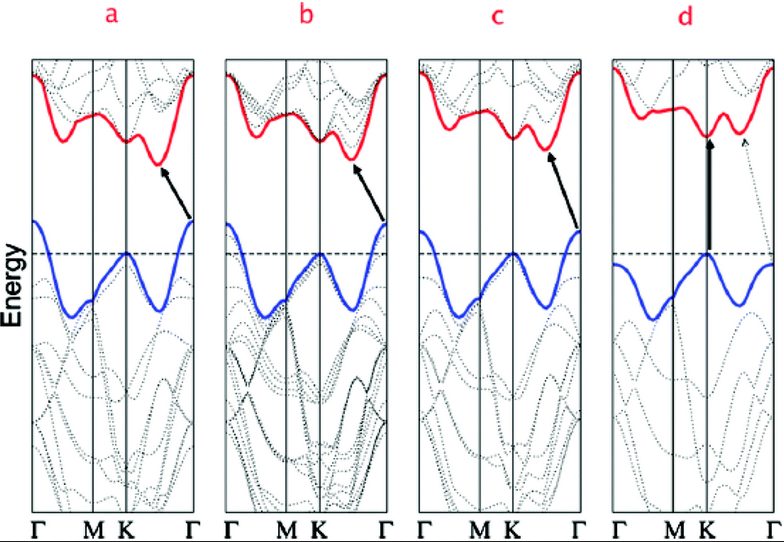
\includegraphics[height=5cm,width=8cm]{figs/intro/mos2_bandstructure}
	\caption[Band structures of \acs{MoS2}]{Calculated band structures of (a) bulk \acs{MoS2}, (b) four-layer \acs{MoS2}, (c) bilayer \acs{MoS2}, and (d) monolayer \acs{MoS2}. Here the solid arrows indicate the lowest energy transitions. (Taken from \cite{Lee_Nanoscale2014}, originally appeared in \cite{Splendiani_Nanolett2010})}
	\label{fig:mos2_bandstructure}
\end{figure}
 
 \begin{table}[ht]
	\centering
	\begin{threeparttable}
	\begin{tabular}{c c c}
		%\hline\hline
		\toprule
		2D material & theoretical $E_g\,(\mathrm{eV})$ & experimental $E_g\,(\mathrm{eV})$ \\ [0.5ex]
		%\hline
		\midrule
		graphene & 0 & 0 \\
		bilayer graphene & 0 & 0\\
		bulk $h$-\ch{BN} & - & 5.97 \cite{Kubota_Science2007}\\
		monolayer $h$-\ch{BN} & - & 6.07 \cite{Kim_NanoLett2011}\\
		few layer (2-5) $h$-\ch{BN} & - & 5.92 \cite{Song_NanoLett2010}\\
		bulk \acs{MoS2} & 1.2\tnote{a,b}\,\,\,\,\, \cite{Mak_PhysRevLett2010,Gourmelon_Solar1997} & 1.0-1.29\tnote{b}\,\,\, \cite{Mak_PhysRevLett2010,Gourmelon_Solar1997}\\
		monolayer \acs{MoS2} & $\sim 1.90$\tnote{a,c}\,\,\,\,\, \cite{Fortin_JournChemSolids1982} & $\sim 1.90$\tnote{b}\,\,\, \cite{Fortin_JournChemSolids1982}\\
		bulk \acs{WS2} & $\sim 1.30$\tnote{a,b}\,\,\,\,\, \cite{Mak_PhysRevLett2010,Kuc_PhysRevB2011} & $\sim 1.35$\tnote{c}\,\,\, \cite{Mak_PhysRevLett2010,Kuc_PhysRevB2011}\\
		monolayer \acs{WS2} & $\sim 2.10$\tnote{a,c}\,\,\,\,\, \cite{Ma_JournChemPhys2011} &-  \\
		bulk \ch{WSe2} & - & $\sim1.20$\tnote{b}\,\,\,\,\, \cite{Wang_NatureNano2012}\\
		monolayer \ch{WSe2} &- & $\sim1.7$\tnote{c}\,\,\,\,\, \cite{Wang_NatureNano2012}\\ [1ex]
		%\hline
		\bottomrule
	\end{tabular}
	\begin{tablenotes}
		\item[a] Theoretical calculations based on first-principles calculations using \ac{DFT}.
		\item[b] Indirect bandgap semiconductor.
		\item[c] Direct bandgap semiconductor.
	\end{tablenotes}
	\caption[Band gaps of typical \acp{TMD} and other materials]{Summary of the bandgaps of typical monolayer, bilayer, and bulk \acp{TMD} and $h$-\ch{BN} materials. Table adapted from ref.~\cite{Xu_ChemRev2013}.}
	\label{table:band_gaps}
	\end{threeparttable}
\end{table}

\section{Current Challenges in \acp{TMD} and Beyond}\label{sec:tmds_and_beyond}
There are several challenges facing the advancement of study of \acp{TMD}. One of these is the development of low contact resistance devices. The formation of a \ac{SB} occurs when making electrical contacts \cite{Fang_NanoLett2012,Das_AppPhysLett2013}. This problem affects many aspects of the growth of \acp{TMD}, low contact resistance devices are essential for the study of intrinsic transport properties and performance limits of devices. Two main approaches exist for achieving low-resistance metal-semiconductor contacts. The first of these is lowering the \ac{SBH} by choosing metals with proper work functions. Finding metals with the proper work function to minimize the \acs{SBH} while still maintaining a high conductivity has proven to be difficult \cite{Liu_ACSnano2012,Das_NanoLett2012}. If a proper work function metal were to be found that met the requirements for current \acs{TMD} performance the effect of lowering the \acs{SBH} may still be diminished due to Fermi level pinning \cite{Gong_NanoLett2014}. Therefore, another method to achieve low-resistance contacts is desirable. The second approach used to achieve low-resistance contacts is to degenerately dope the contact regions. Heavily doping the contact region effectively decreases the \acs{SB} width \cite{Suh_NanoLett2014}. However, this too, has its own challenges associated with it. One possible way to overcome the problems and tune the \acs{SB} is to use a buffer layer and covering with a material such as \hbn or graphene \cite{Geim_Nature2013,Farmanbar_PhysRevB2015,Kappera_NatureMat2014,Farmanbar_arxiv2016}. This second approach has shown promise in reducing the contact resistance and lowering the \acs{SB} while still maintaining high carrier mobility (see ch.~\ref{chap:results}). \\ \\

%\noindent
Aside from the commonly used \td materials like \ch{MoS2} and \ch{WSe2}, \ac{BP} has begun to show promise. Bulk \acs{BP} has a direct bandgap of $\sim 0.3\unita{eV}$, which is expected to increase to $\sim 2.0\unita{eV}$ as the thickness approaches monolayer \cite{Keyes_PhysRev1953,Maruyama_PhysB1981,Tran_PhysRevB2014}. In the past few years, few-layer black phosphorus has been shown to have desireable room temperature field-effect mobility ($\sim 1,000\cmvs$ for $\sim 10$ layer \acs{BP} and $\sim 200\cmvs$ for $5\unita{nm}$ \acs{BP}) \cite{Li_NatureNano2014,Koenig_AppPhysLett2014,Xia_NatureComm2014}. \acs{BP} has shown potential for applications to thin-film electronics and infrared optoelectronics due to its bandgap energy range \cite{Li_NatureNano2015,Xia_NatureComm2014}. In addition, the high mobility measurements have recently allowed for measurements of novel quantum physics, opening the door to further study of intrinsic channel properties of \acp{TMD}.


%\section{Hall Effect}\label{sec:hall_effect}
%Give a brief overview of the history
%\subsection{Overview}\label{subsec:hall_overview}
%\subsection{Theoretical Background}\label{subsec:hall_theory}
%Some useful references for this section \cite{Hall_AmerJournMath1879,Schroder_Semiconductor2006,Kittel_IntroSolidState2005,Ashcroft_SolidStatePhysics1978,Melissinos_Experiments1966,Baumgartner_HallEffect2006} %!!!!!!!!!!!!!uncomment
	\chapter{Experimental Details}\label{chap:exp_details}

\section{Substrate Preperation}\label{sec:sample_prep}
Using degenerately doped \ac{SiO2} wafers that are $270\unita{nm}$ thick as pictured in fig.~\ref{fig:plain_wafer} and the subsequent substrate`s schematic in fig.~\ref{fig:si_sio2_diagram}, there are several preliminary steps needed prior to device fabrication. For easy indentification of locations on the substrate alignment marks are placed on the wafer using photolithography. There is a main alignment mark pictured in fig.~\ref{fig:main_alignment} (REALLY ONLY WANT TO REF A,B) which allows for quicker indentification during electron beam lithography, for example. The alignment marks are in a grid pattern with the coordinate $\left(0,0\right)$ at the center, stretching to $\left(\pm 6,\pm 6\right)$ in both the right and left directions. In each of these coordinate locations there smaller alignment marks evenly spaced within them as shown in fig.~\ref{fig:main_alignment} (FIGURE OUT HOW TO REF SUBFIGS, HERE WE WANT TO REF (c,d)). Next, \ac{Au} is deposited on the surface of the wafer, a process that will be explained in more detail in sec.~\ref{sec:device_fabrication}.
\begin{figure}[ht]
	\centering
	\begin{minipage}[b]{0.25\linewidth}
		\centering
		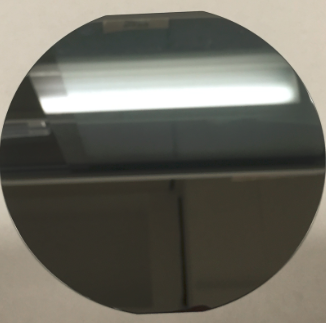
\includegraphics[height=2.5cm,width=2.5cm]{figs/experimental/plain_wafer}
		\caption[Plain wafer]{Plain, polished uncut \ch{Si}/\ch{SiO2} wafer.}
		\label{fig:plain_wafer}
	\end{minipage}
	\qquad
	\begin{minipage}[b]{0.25\linewidth}
		\centering
		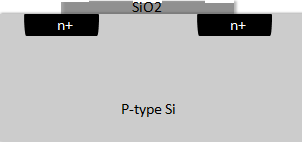
\includegraphics[height=1.75cm,width=3.25cm]{figs/experimental/si_sio2_diagram}
		\caption[Schematic of \ch{Si}/\ch{SiO2} substrate]{Schmatic of \ch{Si}/\ch{SiO2} substrate.}
		\label{fig:si_sio2_diagram}
	\end{minipage}
	\qquad
	\begin{minipage}[b]{0.25\linewidth}
		\centering
		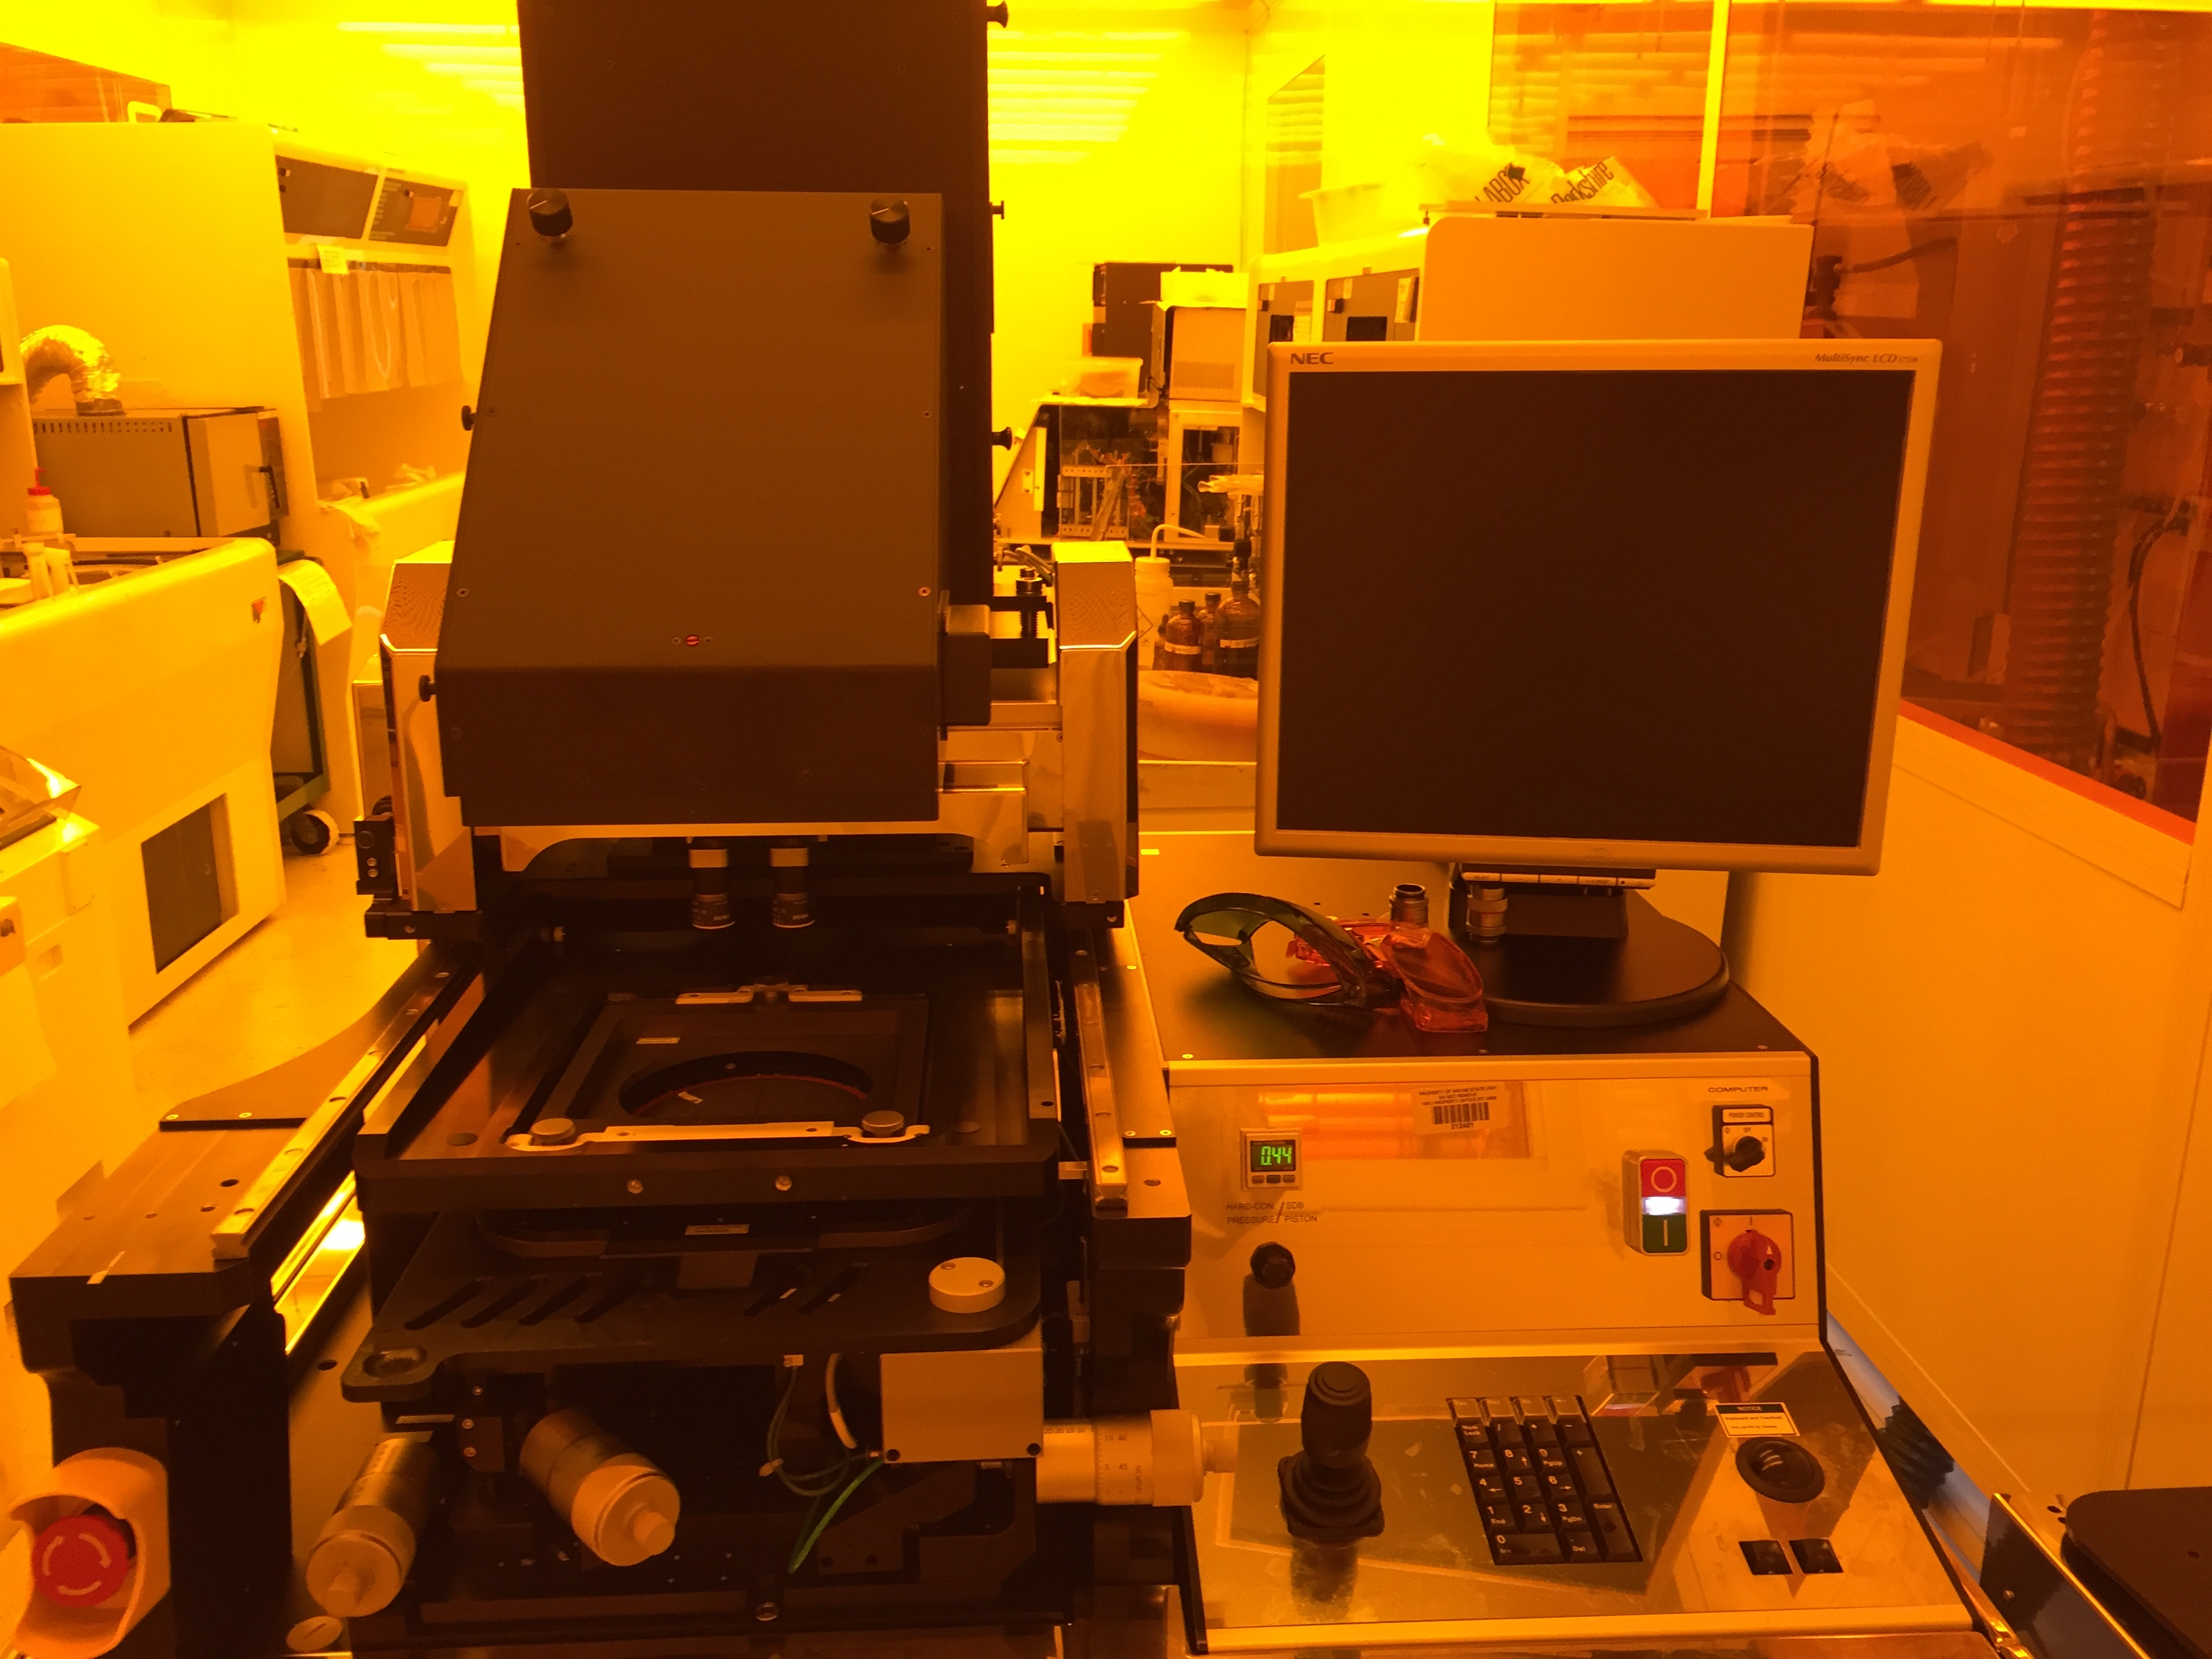
\includegraphics[height=2cm,width=3cm]{figs/experimental/photolithography_bay}
		\caption[Photolithography system]{Photolithography system for creating alignment marks on substrates.}
		\label{fig:photolithography_bay}
	\end{minipage}
\end{figure}
~

\begin{figure}[ht]
	\centering
	\subfloat[Main alignment mark at 5x magnification]{
		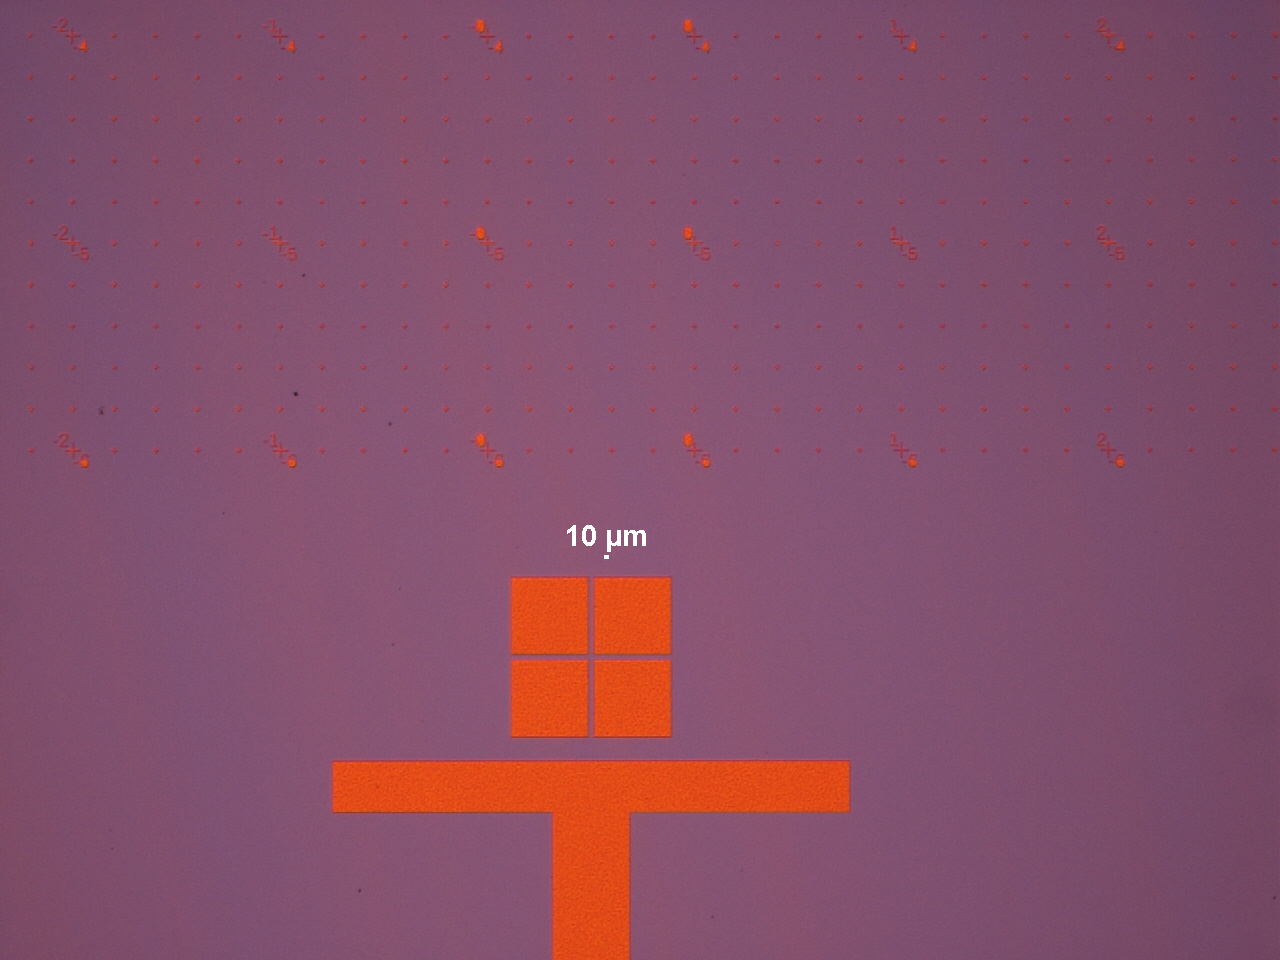
\includegraphics[height=4cm,width=5cm]{figs/experimental/main_alignment_5x}
		\label{fig:main_alignment_5x}
	}
	\qquad
	\subfloat[Main alignment mark at 10x magnification]{
		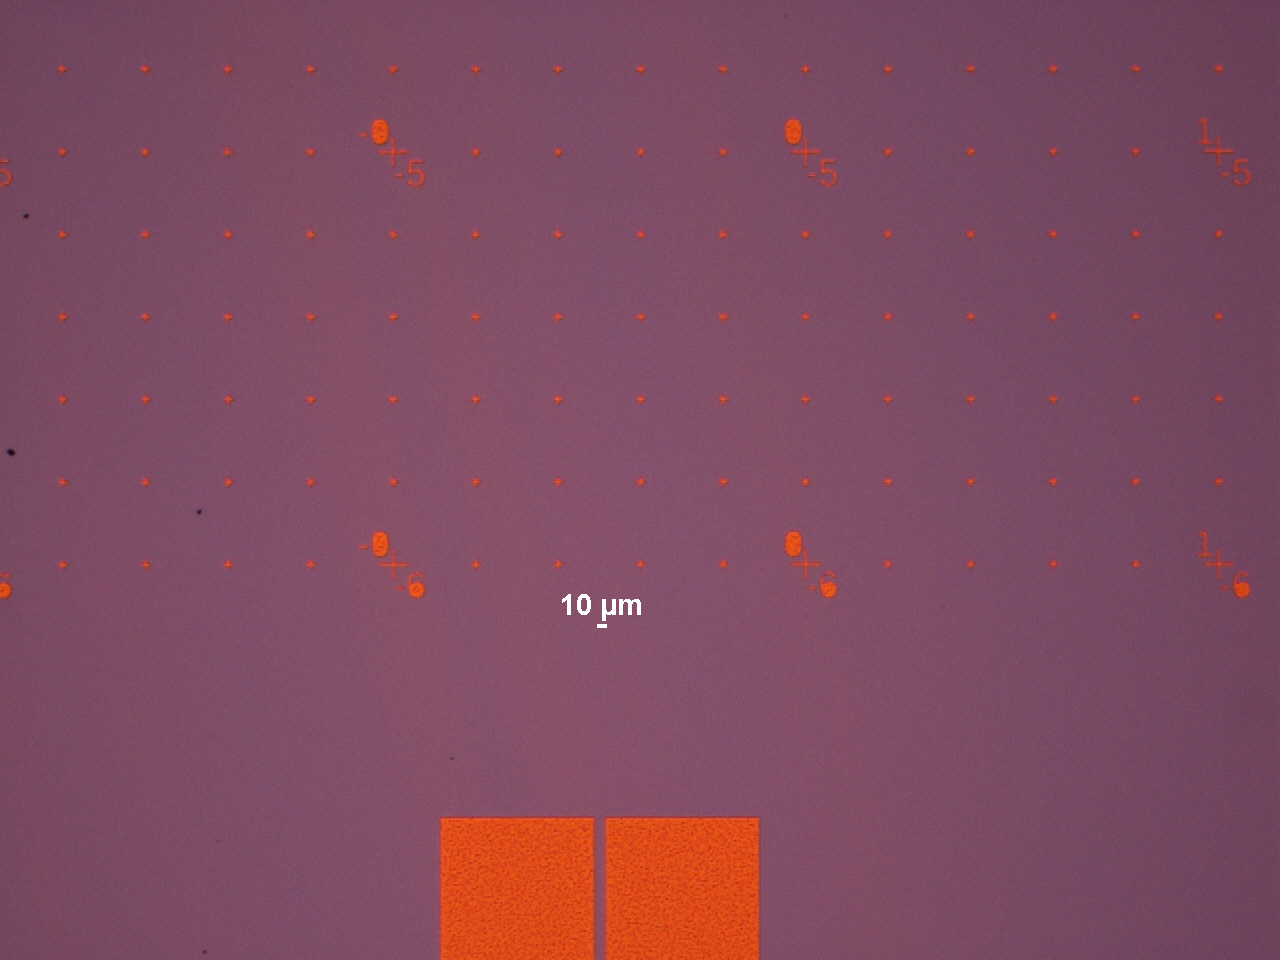
\includegraphics[height=4cm,width=5cm]{figs/experimental/main_alignment_10x}
		\label{fig:main_alignment_10x}
	}

	\subfloat[Coordinate mark $\left(0,-5\right)$ at 50x magnification]{
		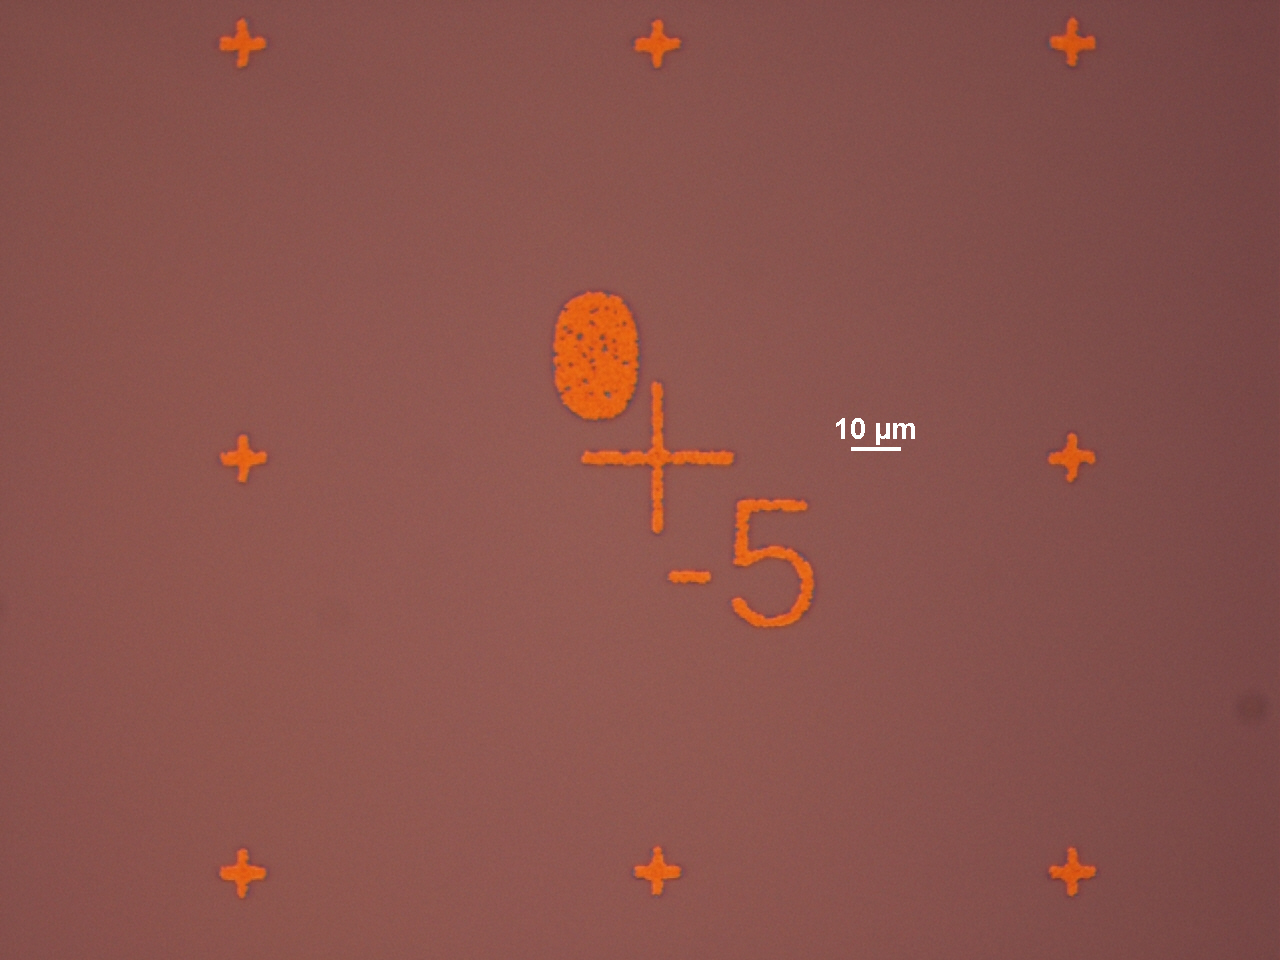
\includegraphics[height=4cm,width=5cm]{figs/experimental/main_alignment_50x}
		\label{fig:main_alignment_50x}
	}
	\qquad
	\subfloat[Coordinate mark $\left(0,-5\right)$ at 100x magnification]{
		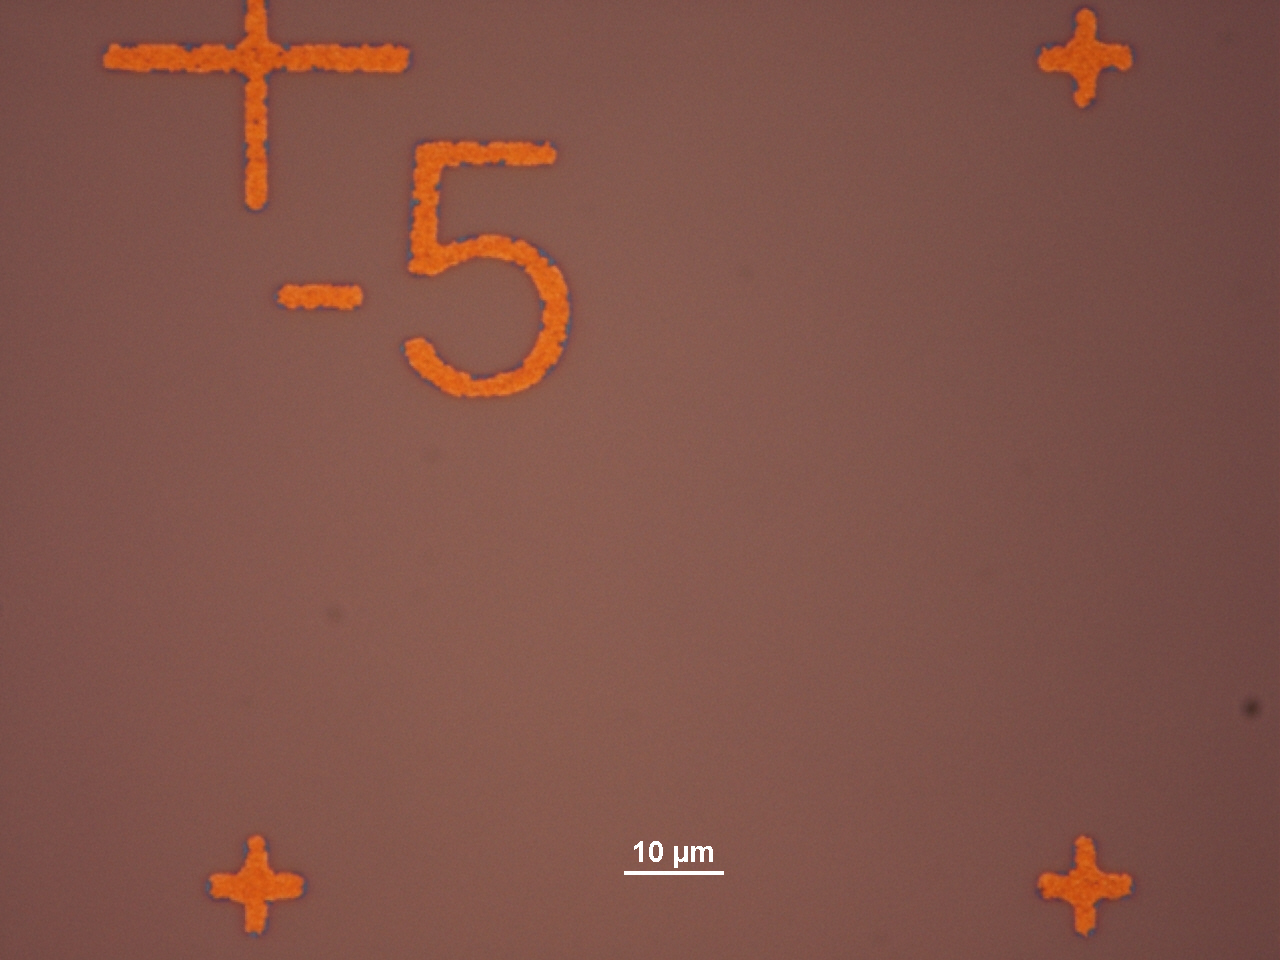
\includegraphics[height=4cm,width=5cm]{figs/experimental/main_alignment_100x}
		\label{fig:main_alignment_100x}
	}
	\caption[Alignment marks at varying magnifications]{Main alignment mark and a coordinate point on a substrate at various magnifications}
	\label{fig:main_alignment}
\end{figure}

%Testing the subref command here \subref*{fig:main_alignment_5x}, \cref{fig:main_alignment_10x}

\subsection{Substrate Cleaning}\label{subsec:cleaning}
Beginning with a cut \acs{SiO2} substrate with a deposited \acs{Au} layer. To remove the \acs{Au} layer, the substrate is first soaked in acetone for approximately 5-10 minutes then washed using \ac{IPA} and dried with \ac{N2} gas. Next, the substrate in placed in acetone and sonicated for 15 minutes. Then sonicated once more but in \acs{IPA} this time with a repition of washing and drying step using \ac{IPA} and \acs{N2} as described above in between each sonication. In order to remove and remaining organic matter on the surface of the substrate, the substrate is annealed under vacuum at $600^\degree\unita{C}$ for 10 minutes and passing forming gas for 2 of the 10 minutes. Forming gas is a mixture of \ch{H2} and an inert gas, usually \ch{N2} \cite{Choi_AppPhysLett2004}. In addition to annealing the substrate for cleanliness, in certain cases when a higher degree of cleanliness is desired the substrate can be treated with oxygen plasma cleaning. 

\section{Exfoliation}\label{sec:exfoliation}
To synthesize samples the most common and often most effective method used is mechanical exfoliation, a technique made famous by the 2004 Novoselov et al. paper. The process involves using Scotch tape to repeatedly cleave layers of \acs{MoS2} or some other TMD. Starting with a crystal of a particular TMD, placing it on a piece of Scotch tape. Then taking another piece of tape and pressing in on the crystal that is on the first piece of tape, being sure to press hard and firm on the crystal. The tape is then lifted up and this process is repeated until the whole piece of tape is filled with small samples of the TMD. At the end of this process it is expected that there are a wide range of mixture of sample sizes in terms of area and in term of thickness as well, where thicknesses of $<3\unita{nm}$ are not uncommon. To better characterize the samples the optical microscope can be used to do so.
\\ \\
\noindent The main challenge that exists with this method is the ability to synthesize a high yield of monolayer samples. This does not seem to be much of a challenge when it comes to graphene and some other TMDs, but with regard to \acs{MoS2} this is not so simple. Based on recently published literature in an effort to increase the yield of monolayer \acs{MoS2} various methods and techniques were tested and modified accordingly \cite{Huang_et_al_ACSnano2015}. In this modified method an additional step to cleaning the substrate is added in which it undergoes oxygen plasma cleaning for 10 minutes to ensure the cleanliness of the substrate`s surface. To promote more bonding between the substrate and the samples, the substrate is first heated at $300^\degree\unita{C}$ for 10 minutes without any samples on it. During this process the normal cleaving of sample on tape from crystal taking place. Once the substrate is done heating the tape containing sample is immediately placed on the substrate and pressed firmly for several minutes. Then the substrate (with the tape still on it) is placed on a glass slide (microscope slide) and is heated at around $85^\degree\unita{C}$ for five minutes. Next, the substrate (with tape) is removed from heat and the tape slowly peeled back from the substrate. The result should be a much higher yield of $<3\unita{nm}$ samples of larger surface area, and several trilayer, bilayer, and a few monolayer samples. (ADD PICTURES OF EACH STEP)
\begin{figure}[ht]
	\centering
	\subfloat[Bulk \ch{MoS2} crystal]{
		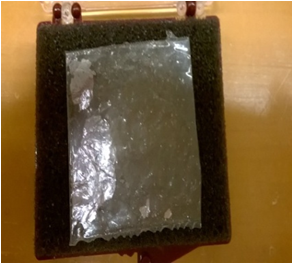
\includegraphics[height=2cm,width=3cm]{figs/experimental/exfoliation_step1}
		\label{fig:exfoliation_step1}
	}
	\qquad
	\subfloat[Single \ch{MoS2} crystal on tape]{
		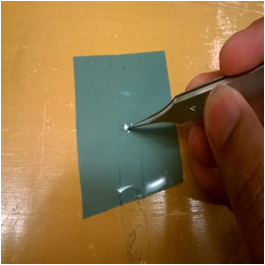
\includegraphics[height=2cm,width=3cm]{figs/experimental/exfoliation_step2}
		\label{fig:exfoliation_step2}
	}
	\qquad
	\subfloat[Tape with exfoliation \ch{MoS2} crystals]{
		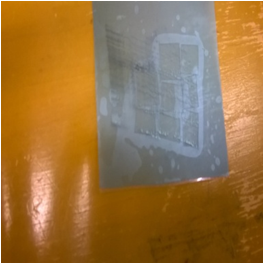
\includegraphics[height=2cm,width=3cm]{figs/experimental/exfoliation_step3}
		\label{fig:exfoliation_step3}
	}
	\caption[Exfoliation steps]{Steps of exfoliation of \ch{MoS2}.}
	\label{fig:exfoliation_steps}
\end{figure}
\\ \\
\noindent Most commonly \acs{SiO2} substrates are the main items that are exfoliated onto. However, depending on the material being synthesized, this may not always be the case. In cases where samples of \hbn or in the event that the thickness of the synthesized sample is not of great importance and can to tolerated up to $20-30\unita{nm}$, \ac{PDMS} is exfoliated onto instead of \acs{SiO2} substrates. The resulting samples are of varying thickness, on average around $20\unita{nm}$. Thin samples (usually trilayer and above) can be made using this method of \acs{PDMS}, however, these samples tend to have small surface area and lack uniformity which poses problems as to their usability. As such, this remains an effective method for obtaining samples in which thickness is not the main concern. Once the samples have been optically characterized, the sample(s) on \acs{PDMS} must be transferred to a \acs{SiO2} substrate.

\section{Device Synthesis}\label{sec:synthesis}
Once the sample or samples have been synthesized and characterized for their specific purpose these samples can begin to be synthesized into a device for measurement. Generally, this involves the technique of transfer. Transfer is usually done using the aforementioned \acs{PDMS} or using \ac{PC} known as the \acs{PC} pickup method. Each method has its advantages and disadvantages depending on the type of sample, type of device, or any number of the factors.
%
\subsection{\acs{PDMS} Transfer}\label{subsec:pdms_transfer}
\acs{PDMS} transfer is most useful for samples that were originally exfoliated onto \acs{PDMS}, for example \hbn. To manufacture \acs{PDMS} a 10:1 ratio of silicone base and curing agent is mixed together and placed in vacuum for 30 minutes to ensure the removal of any remaining air bubbles. After this time the mixture is then spin coated on a plain \acs{SiO2} wafer and heated at $80^\degree\unita{C}$ for 30 minutes then allowed to cool for 30 minutes. Once cooled, the surface of the wafer can be cut using a razor into small stamps that can used for exfoliation and for transfer. \\ \\
\noindent Once the samples that are to be transferred are on the \acs{PDMS} stamp, then it is placed on a glass slide. Using the optical microscope to locate the sample on the stamp and using a razor to cut small excess pieces from the portions of the stamp where the desired sample is not located. This process is repeated until the size of the cut stamp is now reasonably small. The cut stamp is then placed at the edge of a new glass slide with sample area of the stamp as close to the edge as can be and the other side of the stamp is taped down using Scotch tape. \\ \\
\noindent Next a substrate is placed and secured using glue (usually PMMA) to the stage of the transfer setup. The transfer stage setup is pictured in fig.~\ref{fig:transfer_stage_setup}. It consists of a microscope that has the capability of 10x or 20x magnification and a micro-manipulator. The micro-manipulator is where the glass slide with the \acs{PDMS} stamp is placed. Using the manipulator the substrate on the stage is approached and the position of the stamp is checked and re-checked multiple times using the microscope to ensure correct overlap of the desired portion of the sample(s). Upon reaching the desired position, the glass slide is lowered but this time there should be a contrast seen which is the overlapping of the glass slide and the substrate. Once the contrast has enveloped the entire sample that was to be transferred then the manipulator can be used to lift up the glass slide. Once the transfer is complete then the substrate should be annealed at $250^\degree\unita{C}$ for 30 minutes in order to remove and residue or orgranic matter that may have remained during the transfer process.
\begin{figure}[ht]
	\centering
	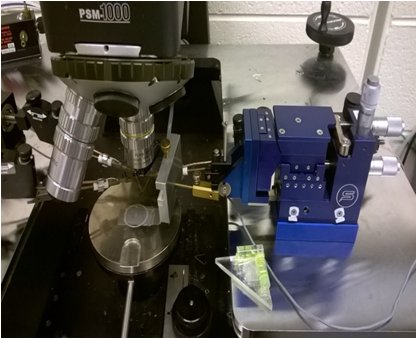
\includegraphics[height=5cm,width=5cm]{figs/experimental/transfer_stage_setup}
	\caption[Transfer stage setup]{Transfer stage setup}
	\label{fig:transfer_stage_setup}
\end{figure}
\subsection{Polycarbonate Pickup Method}\label{subsec:pc_pickup}
The PC pickup method is used for samples that have been exfoliated onto a \acs{SiO2} substrate. Generally these are thinner samples with larger surface area that are not as easily obtained by using the PDMS exfoliation method as described in sec.~\ref{sec:exfoliation}. To manufacture the PC, $3.0\unita{g}$ of chloroform and $0.18\unita{g}$ of polycarbonate resin are put on a plate shaker for about 60 minutes or until the polycarbonate resin have dissolved into the solution. \\ \\
\noindent Next, the substrate that has the sample that is going to be transferred in taped using double-sided tape to a glass slide facing up. Then using a syringe the \acs{PC} solution is placed in the substrate and evenly spread across it. Being sure to locate the area(s) on the substrate where the sample(s) are located, small pre-cut pieces of PDMS are placed over top of these areas. An outline of the \acs{PDMS} stamps is cut using a razor and any excess \acs{PDMS} is carefully torn away. Once only the \acs{PDMS} strips are remaining on the substrate \ac{DI} is put under the strips in order to create a hydrophobic surface and to ensure that the strip and PC that is trapped underneath it come off the substrate with relative ease. Each strip is placed on its own glass slide and is gently blown with \ch{N2} gas to remove any excess \acs{DI} from the surface. \\ \\
\noindent Moving to the transfer stage setup and following the steps described in sec.~\ref{subsec:pdms_transfer} with regard to using the transfer stage setup. The only difference at this point to using this method as opposed to \acs{PDMS} transfer is in the final step of the transfer. Instead of only lowering until the contrast change is shown between the region that is desired to be transferred, with PC transfer the entire PC must be lowered down. This is because since the PC will be heated before being lifted up. Lowering all the way ensures that all the PC will be melted. Once lowered all the way, the heating device, which is connected to the stage, should be turned up to $130^\degree\unita{C}$. Once this temperature is reached, it should be maintained for approximately two minutes to fully melt the PC film. After heating the substrate and lifting up using micro-manipulator the substrate is placed in chloroform and covered for 30-60 minutes. The purpose of this is to remove any residue left over by the PC film or any other items that may have been introduced at any point in the transfer process. In practice the chloroform soaking generally needs to be repeated several times over a few hours in order to ensure the least amount of remaining residue possible. To confirm the reduction of residue and also characterize the transferred samples an AFM is used. 

\section{Characterization}\label{sec:characterization}
There are many ways used in modern academia and industry to characterize samples and devices. Some of these methods include \ac{STM}, \ac{TEM}, \ac{AFM}, and \ac{MFM} \cite{Kittel_IntroSolidState2005}. The primary characterization techniques used in this project are \acs{AFM} and optical characterization.
\subsection{Optical Characterization}\label{subsec:characterization_optical}
The majority of the optical characterization is carried out using the optical microscope as shown in figs.~\ref{fig:optical_microscope_front_view} and~\ref{fig:optical_microscope_side_view}. The microscope can magnify 5x, 10x, 20x, 50x, and 100x, in addition, it can show dark field images.
\begin{figure}[ht]
	\centering
	\begin{minipage}[b]{0.45\linewidth}
		\centering
		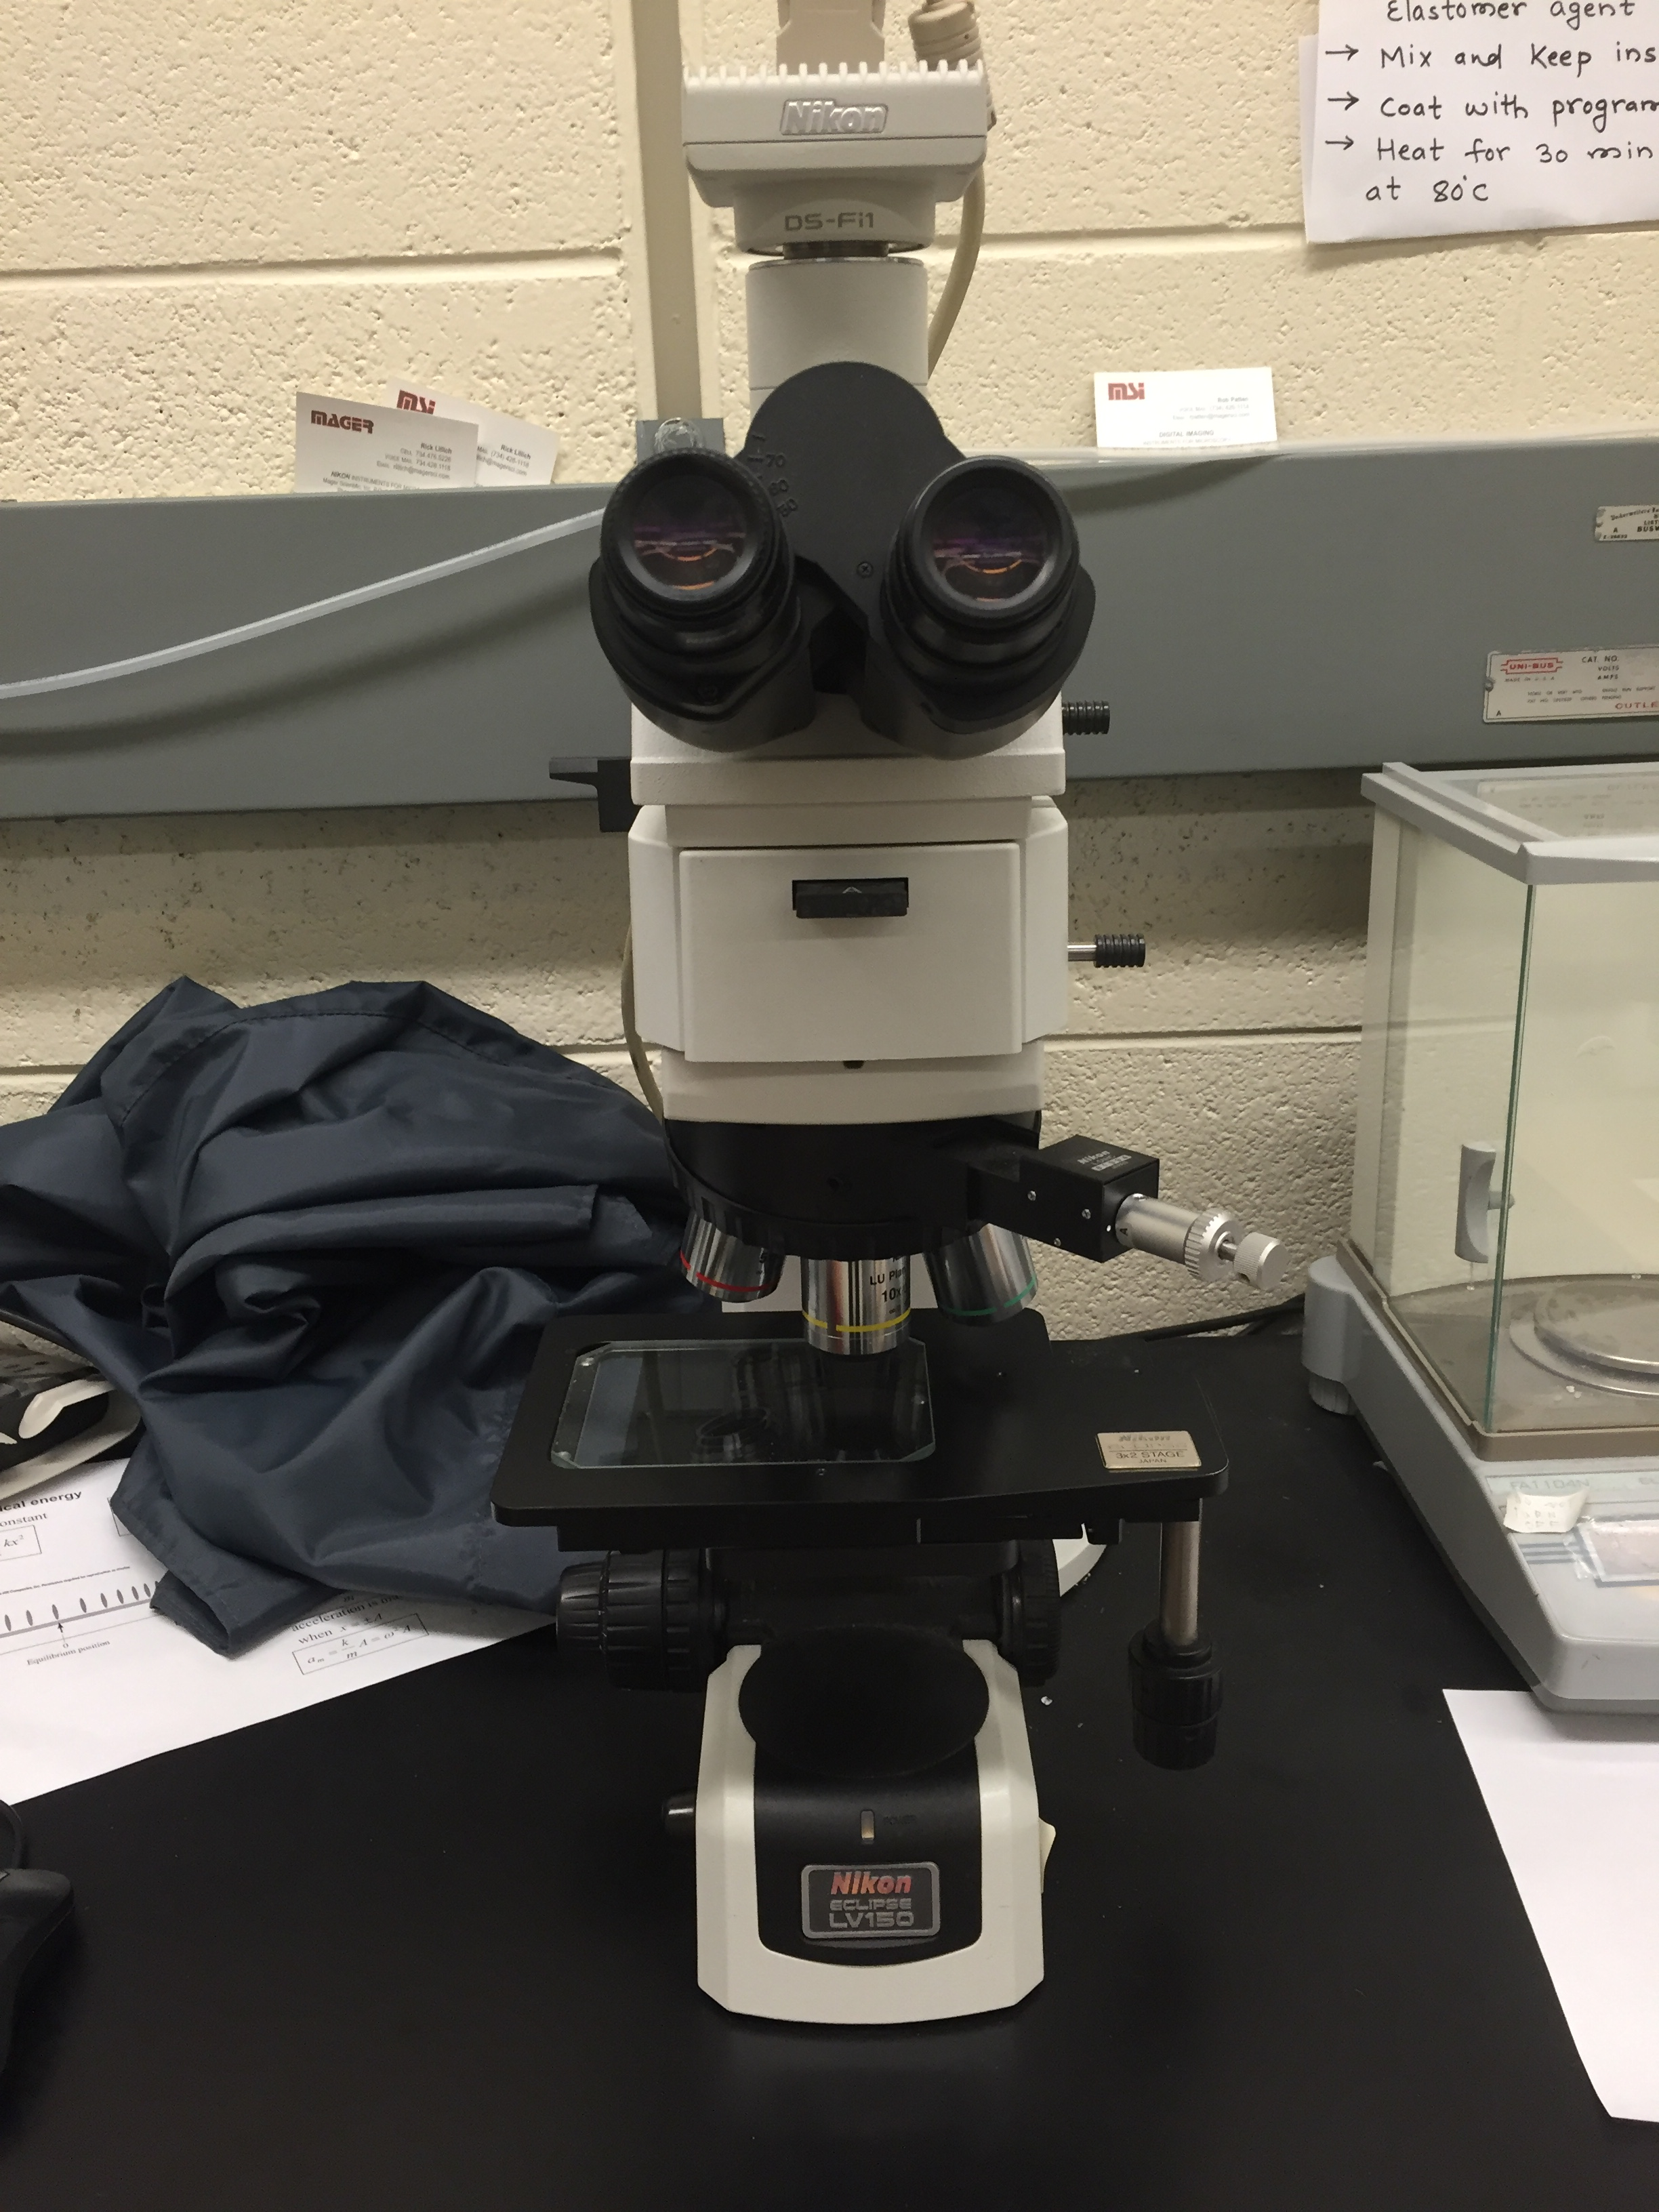
\includegraphics[height=5cm,width=5cm]{figs/experimental/optical_microscope_front_view}
		\caption[Optical microscope front view]{Optical microscope front view}
		\label{fig:optical_microscope_front_view}
	\end{minipage}
	\qquad
	\begin{minipage}[b]{0.45\linewidth}
		\centering
		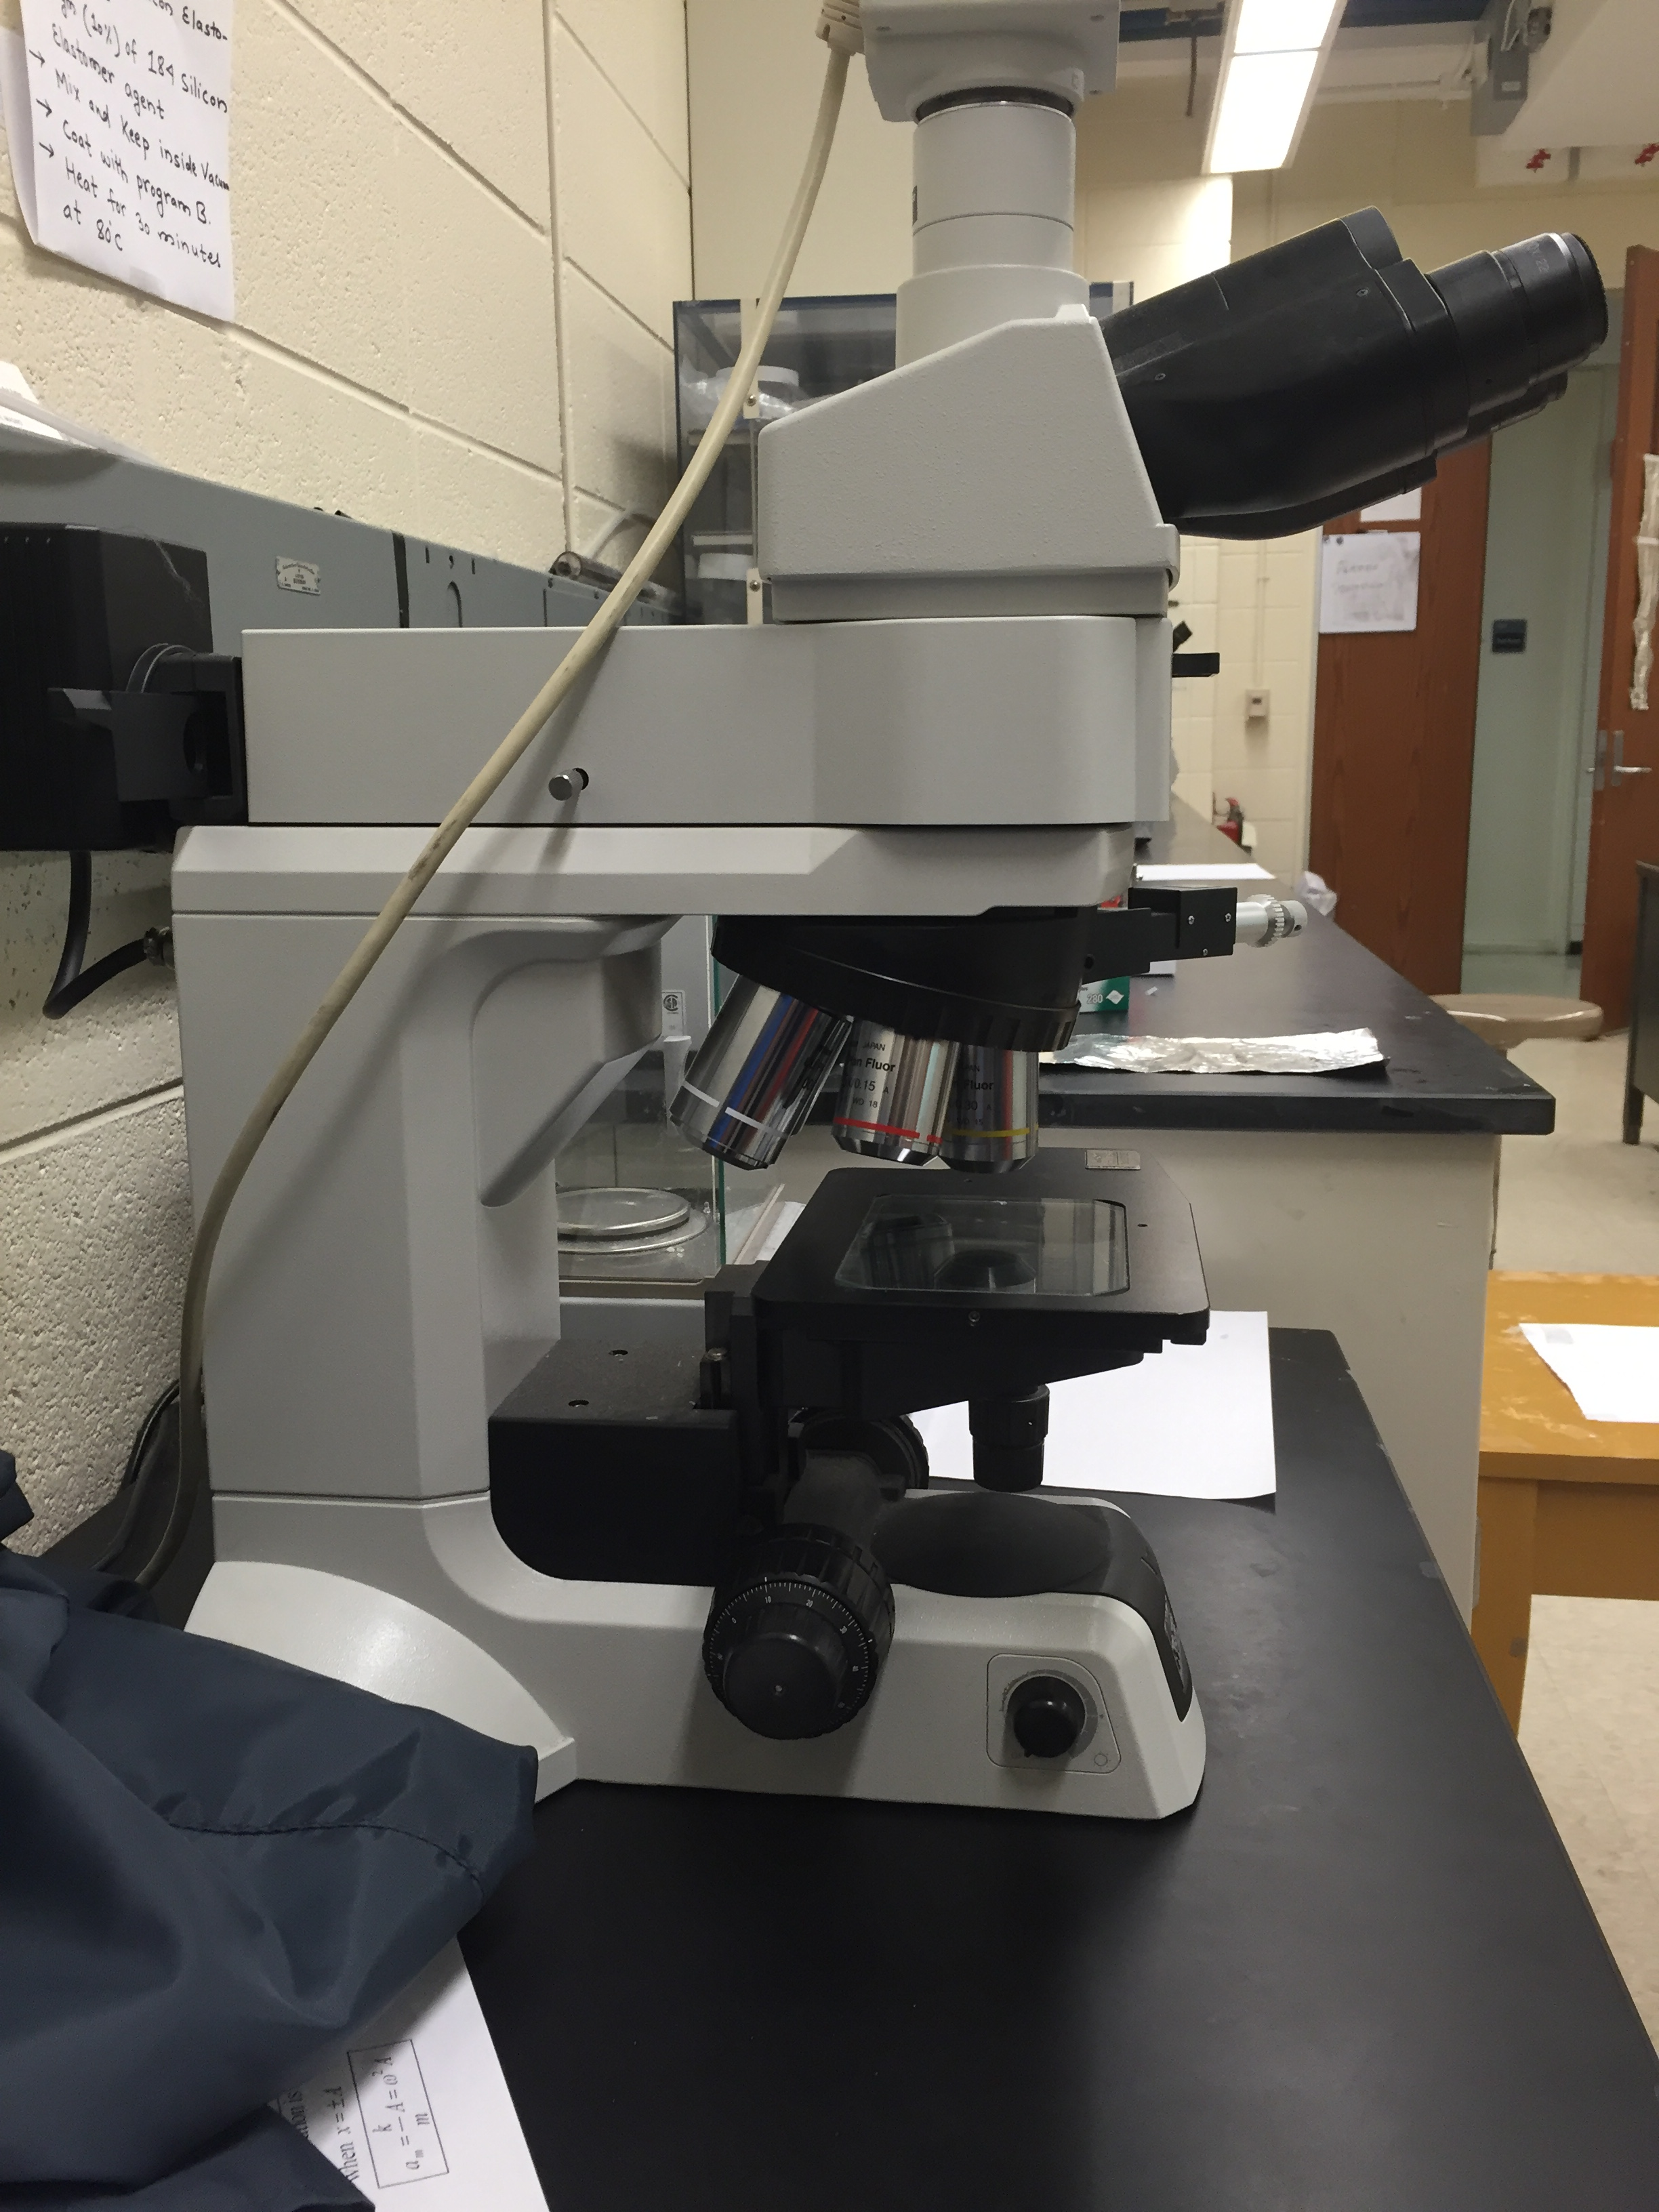
\includegraphics[height=5cm,width=5cm]{figs/experimental/optical_microscope_side_view}
		\caption[Optical microscope side view]{Optical microscope side view}
		\label{fig:optical_microscope_side_view}
	\end{minipage}
\end{figure}

\subsection{AFM Characterization}\label{subsec:characterization_afm}
In addition to the characterizing samples optically, \acs{AFM} characterization is another important aspect of the device design and fabrication process. \acs{AFM} characterization occurs several times throughout the process, after each transfer of a sample onto another, for example. This occurs for two reasons; to verify the thickness of the sample(s) that have been transferred, and also to verify the cleanliness of the surface of the sample (to ensure that any residue has been removed, especially during the course of PC transfer). Additionally, once the electrodes of the device have been fabricated a final \acs{AFM} characterization is need to determine the width of the device`s channel which is needed to calculate various important electrical properties. \\ \\

\noindent Fig.~\ref{fig:afm_front_view} shows a front view of the \acs{AFM} used to characterize. For these purposes, the \acs{AFM} is operating in ``tapping" mode which is less invasive than ``contact" mode \cite{Kittel_IntroSolidState2005}. In basic terms, an \acs{AFM} works by measuring the force between the tip of a cantilever (see fig.~\ref{fig:AFM_tip}) and the sample being imaged. 
\begin{figure}[ht]
	\centering
	\begin{minipage}[b]{0.45\linewidth}
		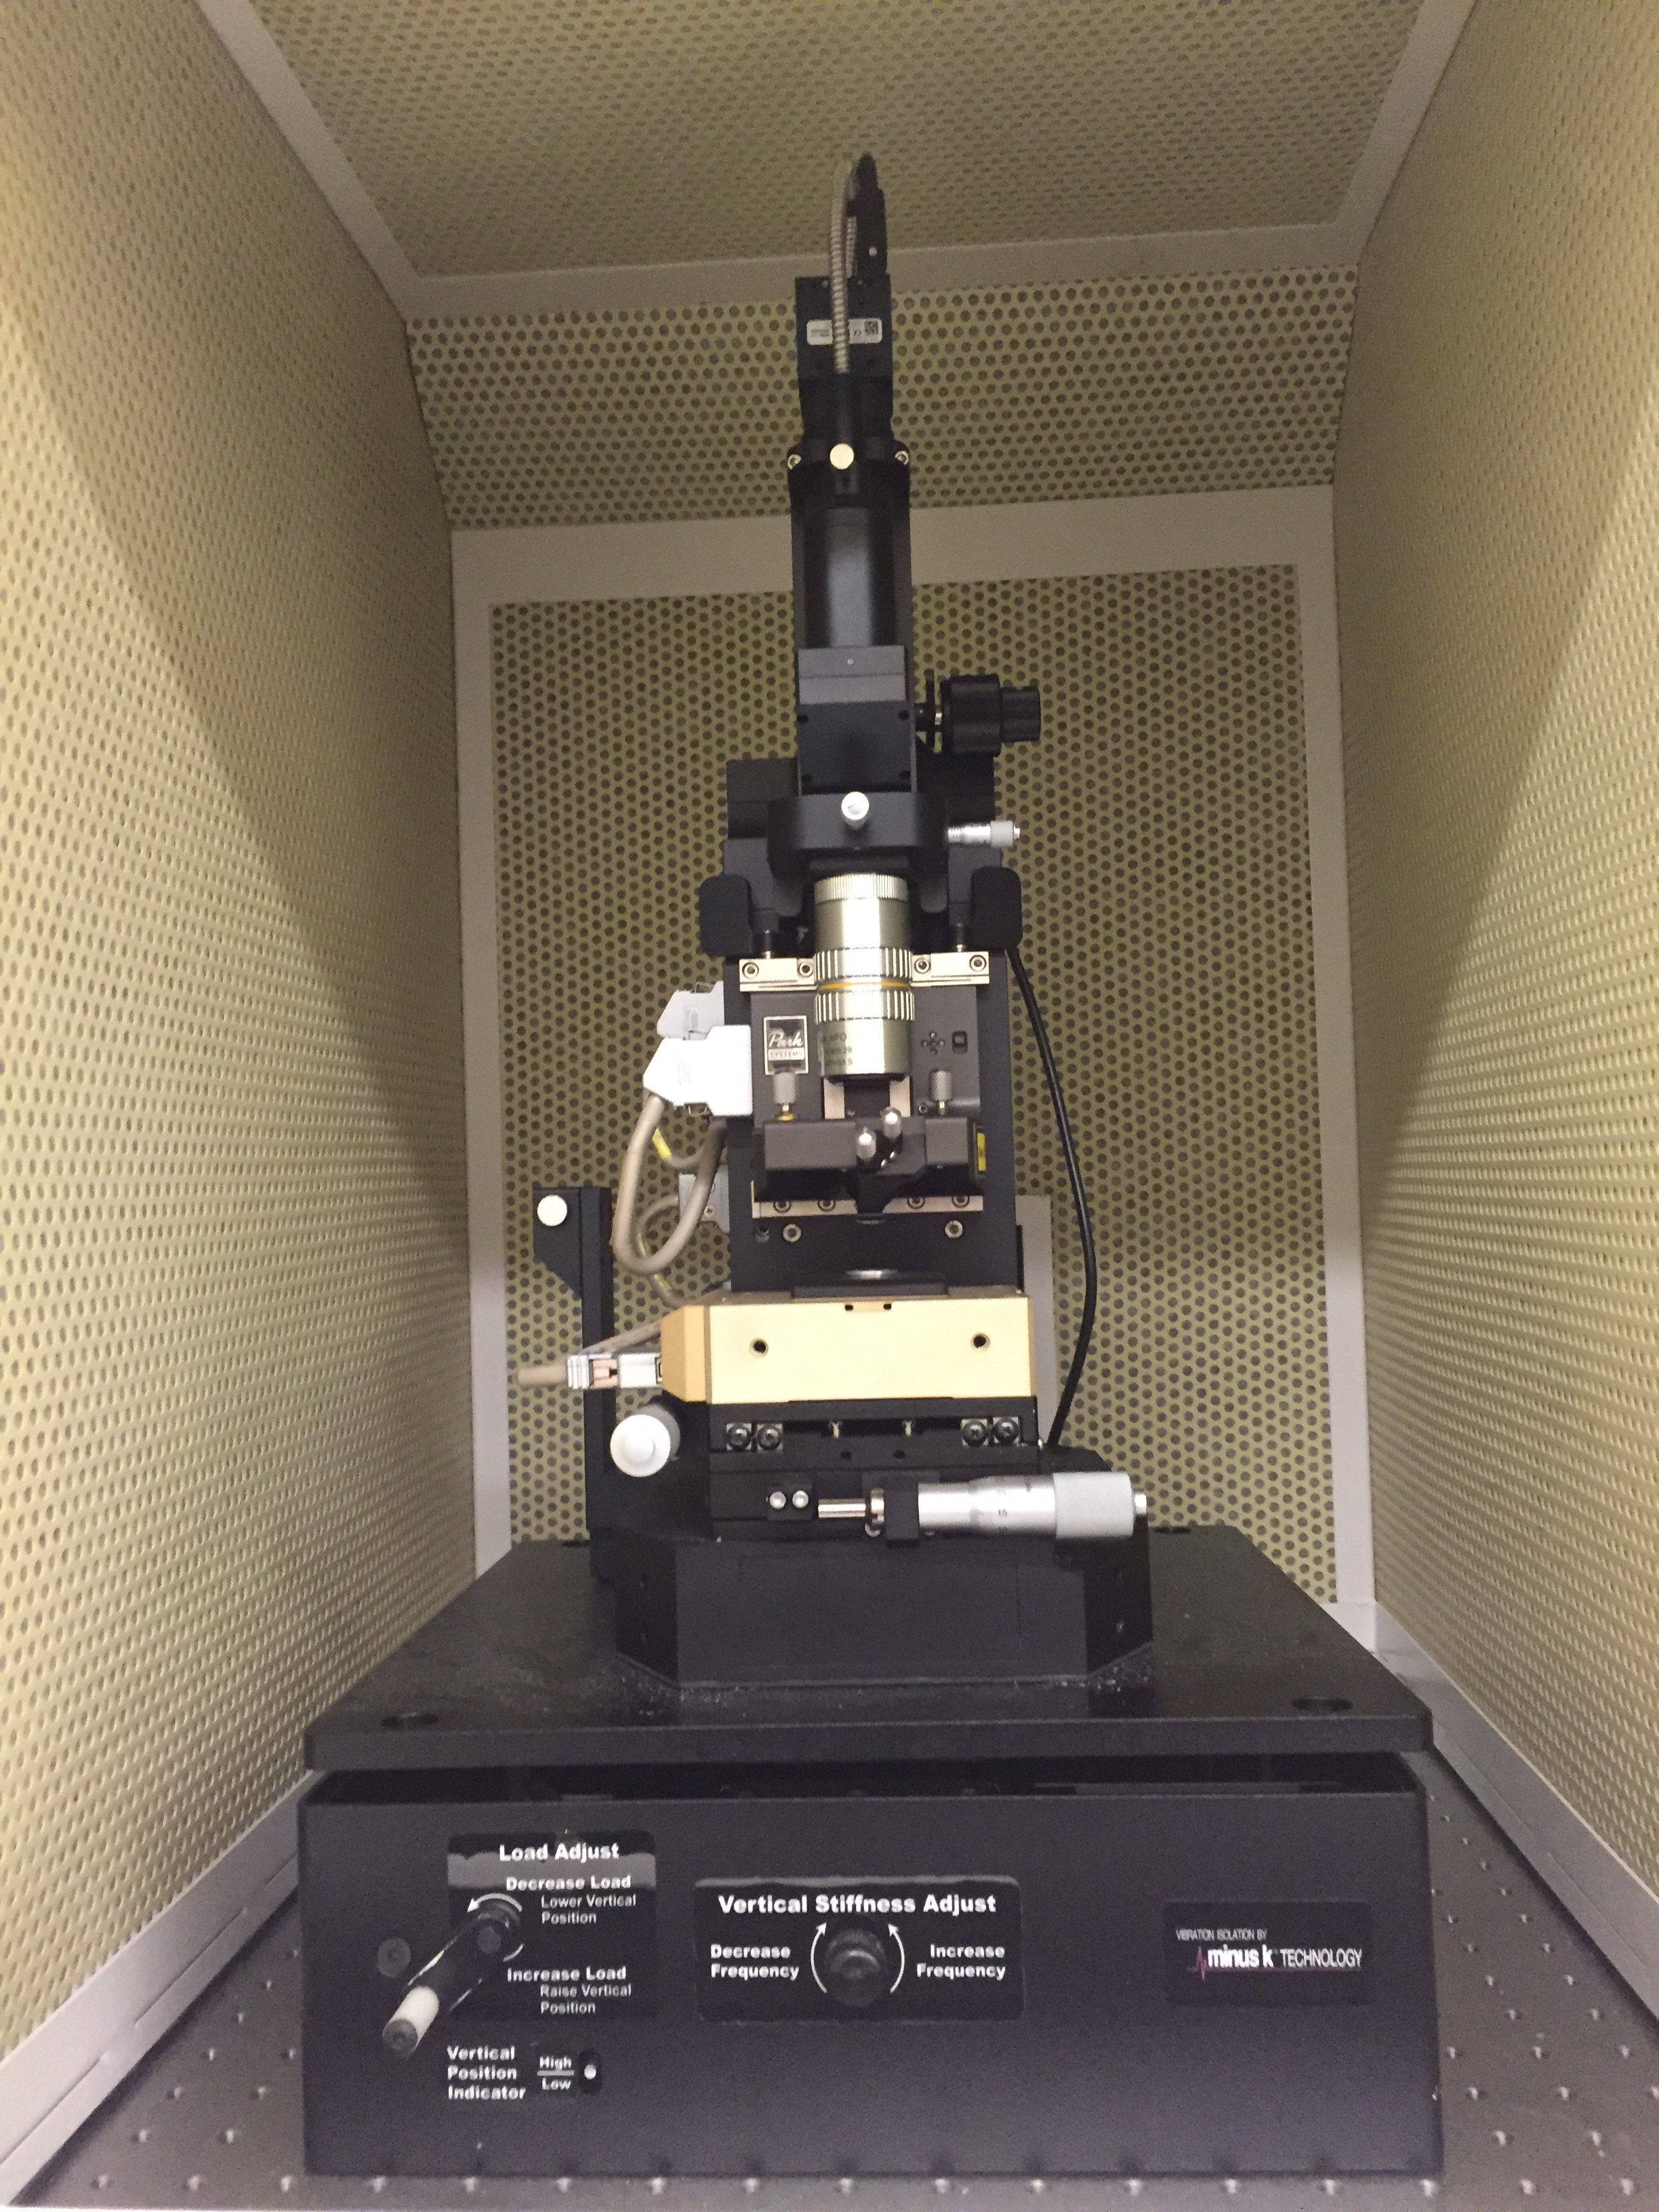
\includegraphics[height=4cm,width=4cm]{figs/experimental/AFM_front_view}
		\caption[AFM front view]{AFM front view}
		\label{fig:afm_front_view}
	\end{minipage}
	\qquad
	\begin{minipage}[b]{0.45\linewidth}
		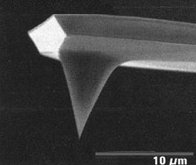
\includegraphics[height=4cm,width=4cm]{figs/experimental/AFM_tip}
		\caption[AFM cantilever]{AFM cantilever \cite{Ernst-Moritz-Arndt_Online}}
		\label{fig:AFM_tip}
	\end{minipage}
\end{figure}

\section{Device Fabrication}\label{sec:device_fabrication}
\subsection{Device Design}\label{subsec:device_design}
\subsection{Electron Beam Lithography}\label{subsec:lithography}
\begin{figure}[ht]
	\centering
	\includegraphics[height=3cm,width=5cm]{figs/experimental/SEM}
	\caption[Scanning electron microscope]{Control panel and electron beam writer of scanning electron microscope.}
	\label{fig:SEM_machine}
\end{figure}

\begin{figure}[ht]
	\centering
	\subfloat[Developed pattern 10x]{
		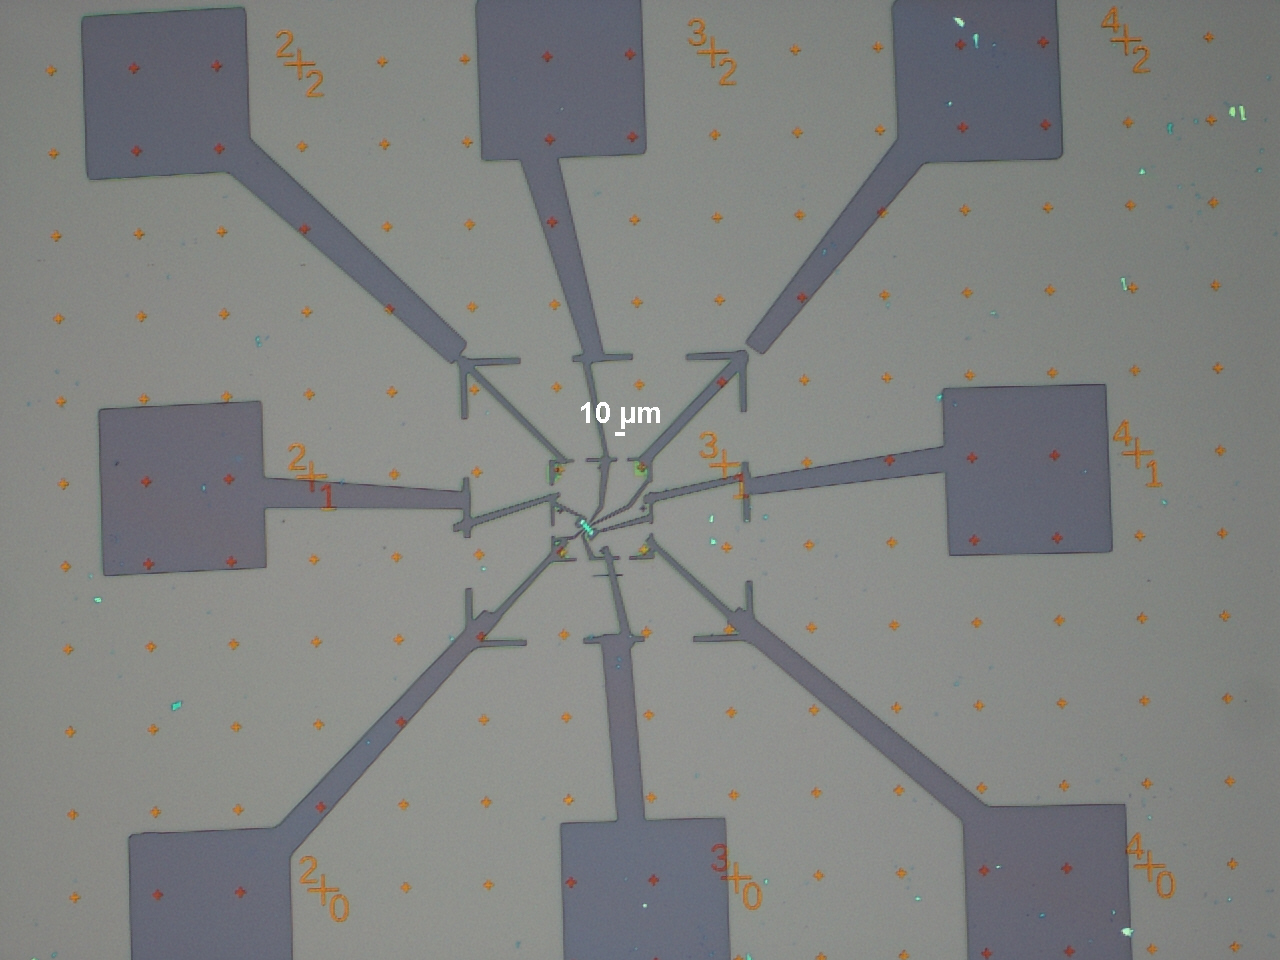
\includegraphics[height=4cm,width=4cm]{figs/experimental/ebeam_developed_10x}
		\label{fig:ebeam_developed_10x}
	}
	\qquad
	\subfloat[Developed pattern 100x]{
		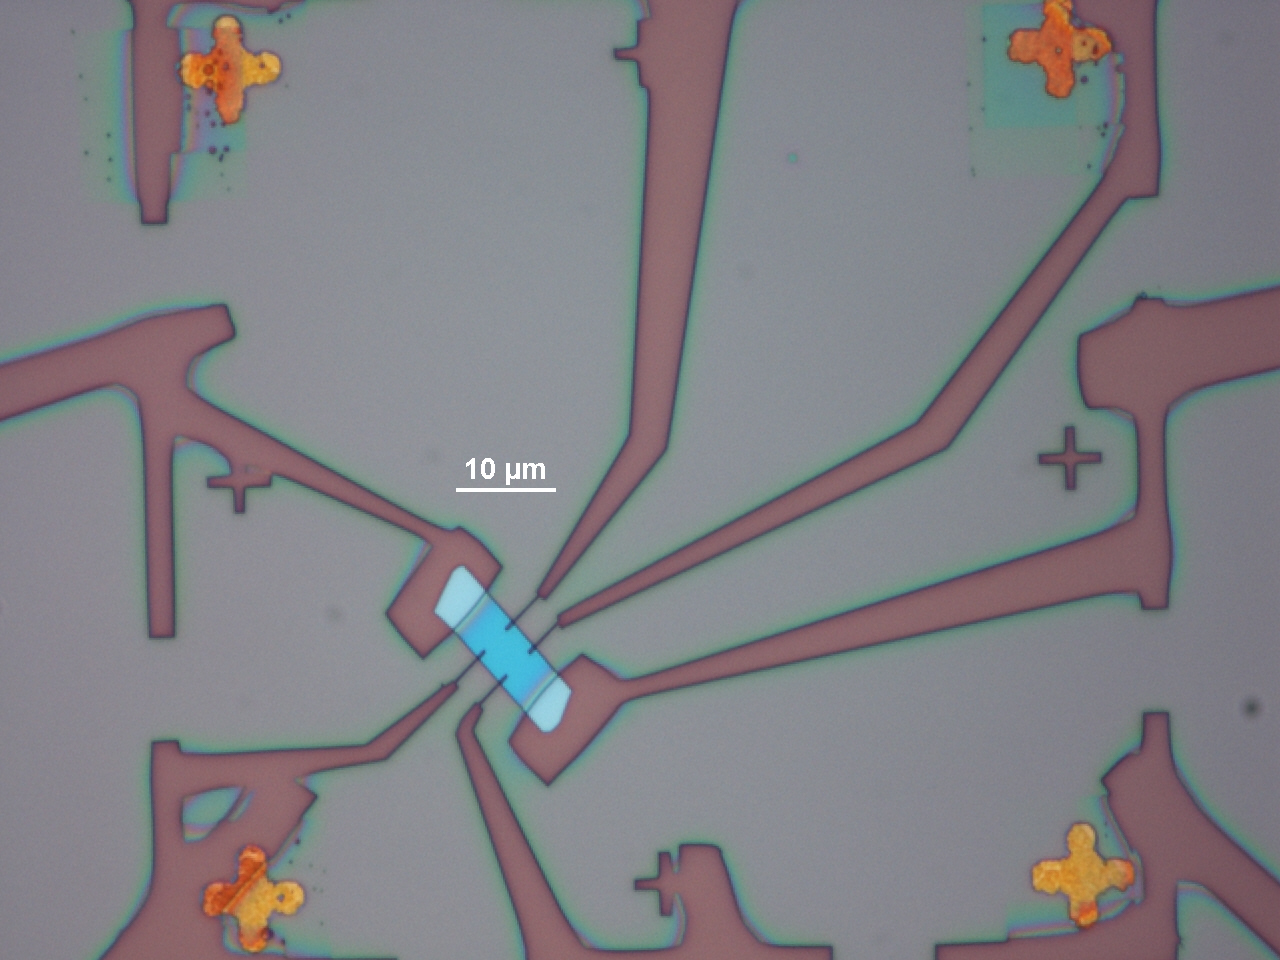
\includegraphics[height=4cm,width=4cm]{figs/experimental/ebeam_developed_100x}
		\label{fig:ebeam_developed_100x}
	}
	\caption[Electron beam lithography patterns]{10x and 100x electron beam lithography patterns developed using \acs{MIBK} and \acs{MEK}.}
	\label{fig:ebeam_developed}
\end{figure}

\subsection{Metal Deposition}\label{subsec:deposition}
\begin{figure}[ht]
	\centering
	\begin{minipage}[b]{0.45\linewidth}
		\centering
		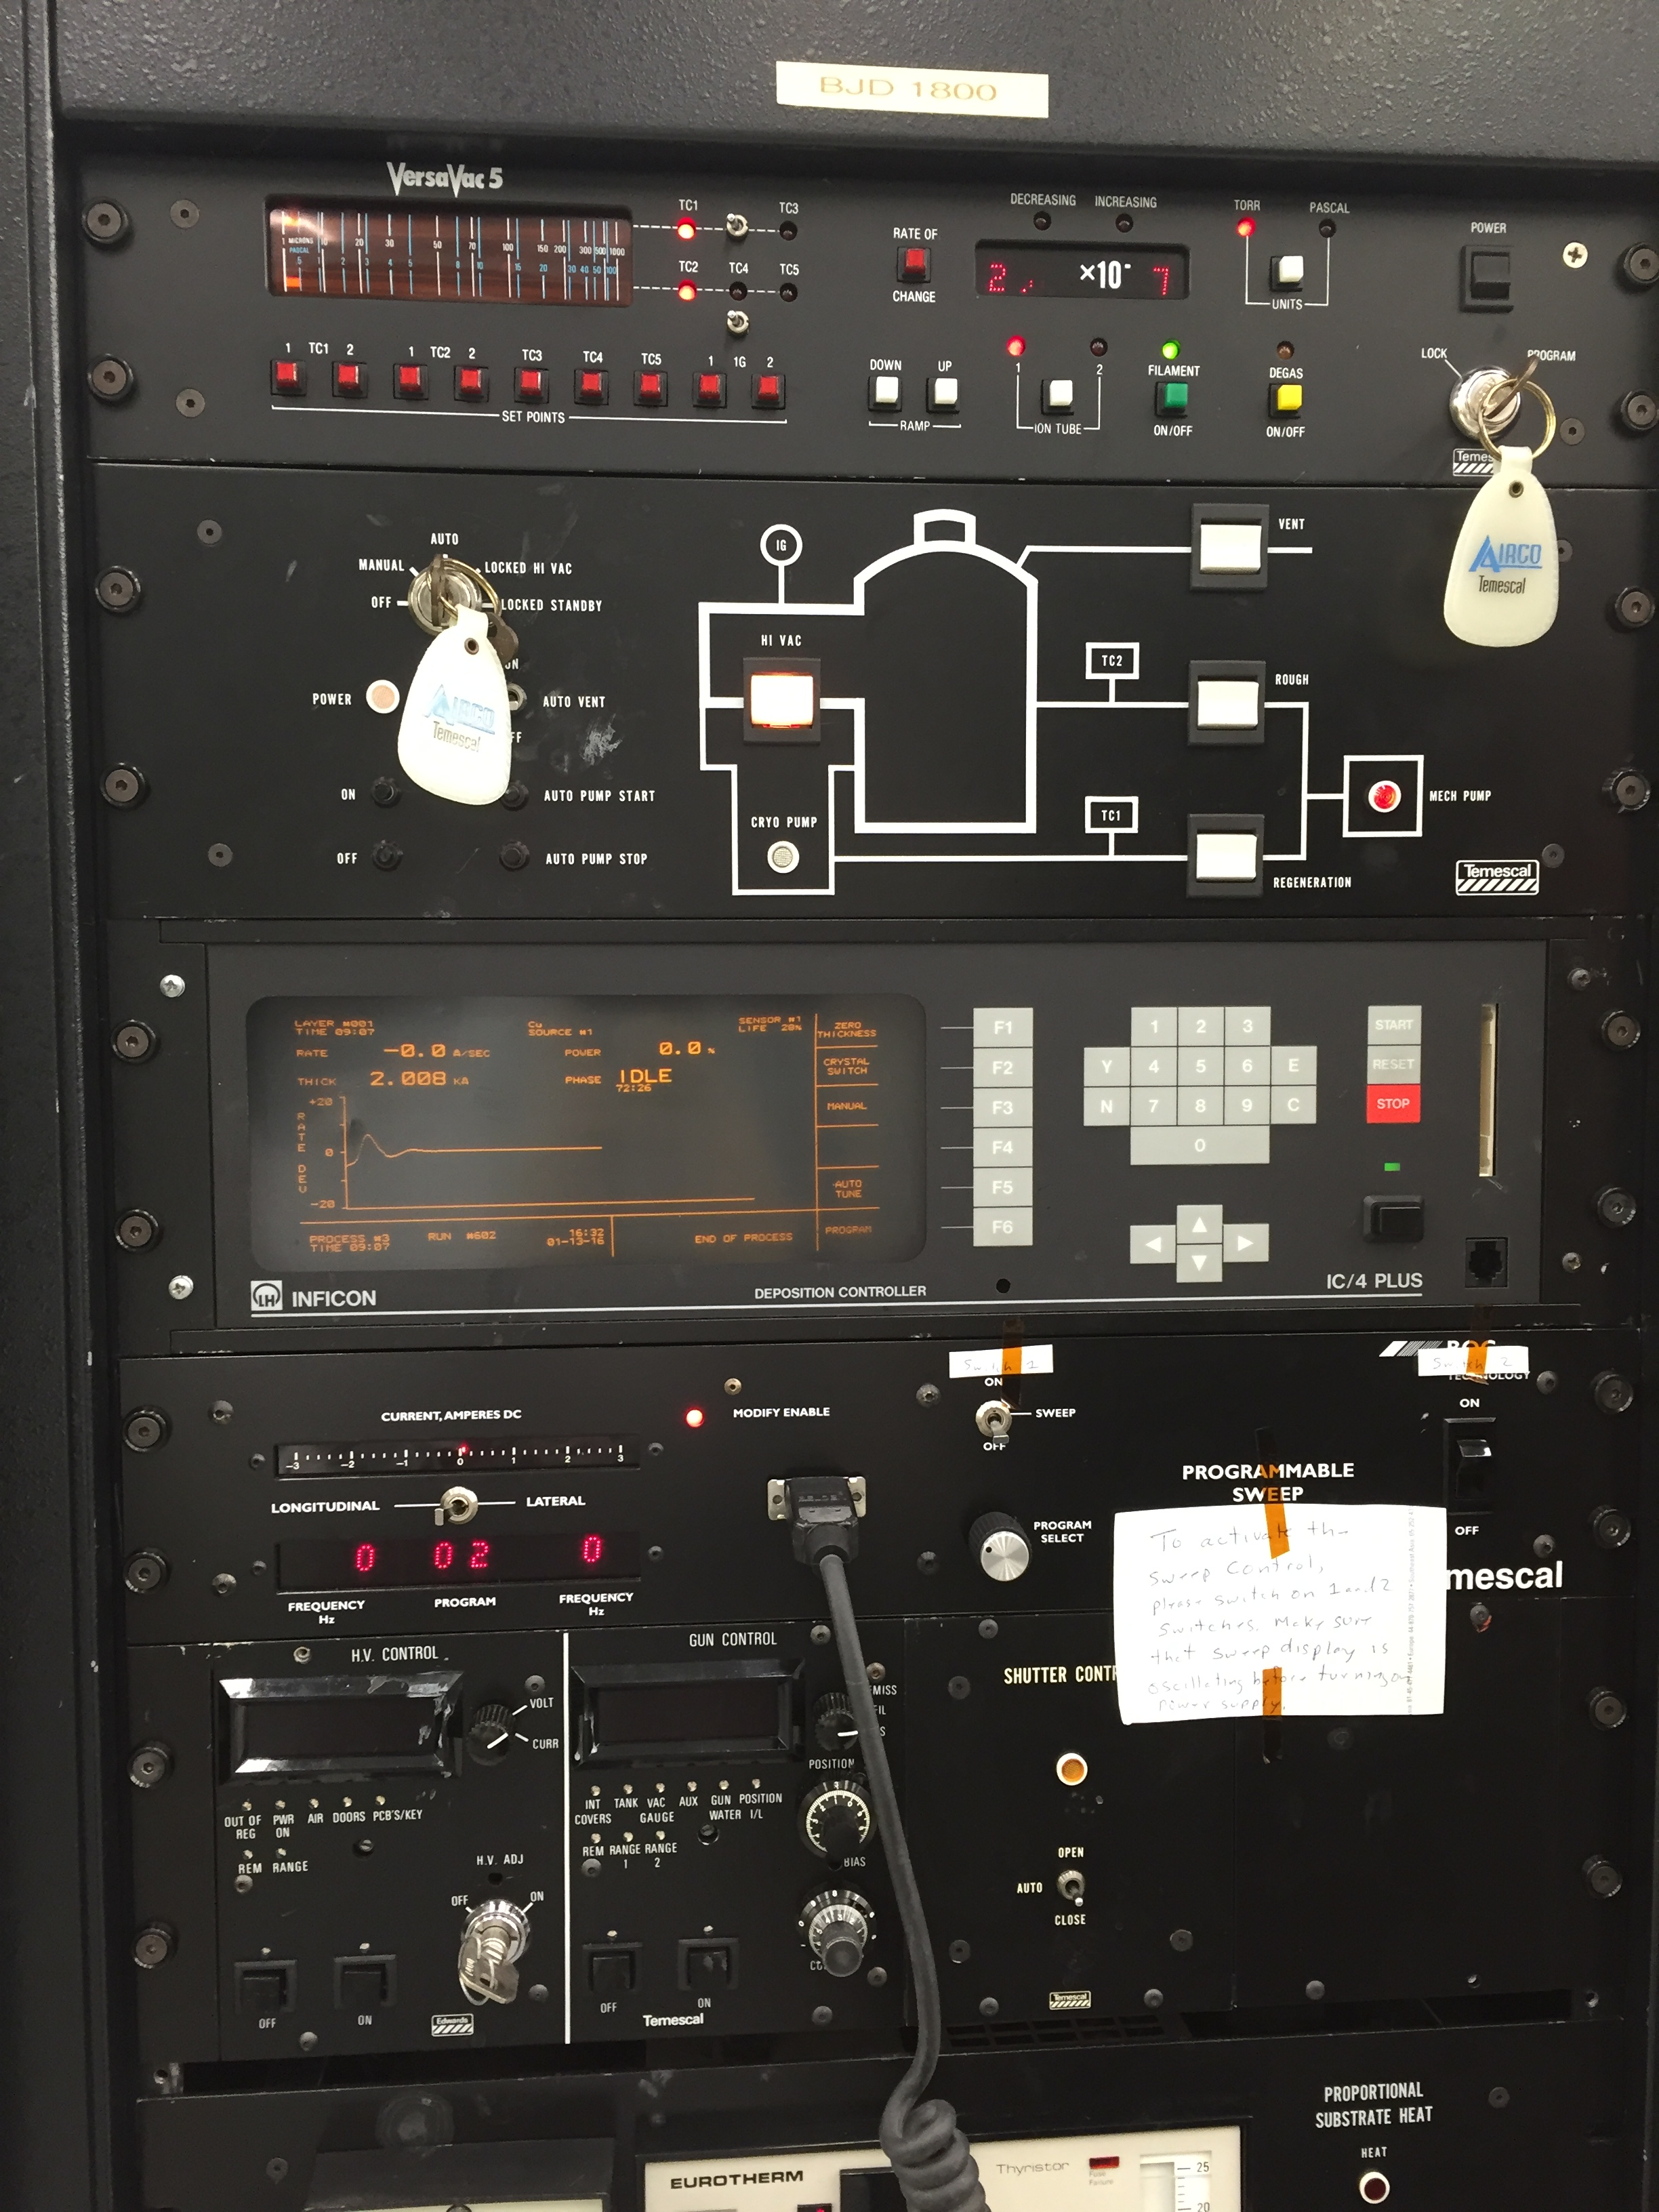
\includegraphics[height=4cm,width=4cm]{figs/experimental/bjd_control_panel}
		\caption[BJD control panel]{caption 1}
		\label{fig:bjd_control_panel}
	\end{minipage}
	\qquad
	\begin{minipage}[b]{0.45\linewidth}
		\centering
		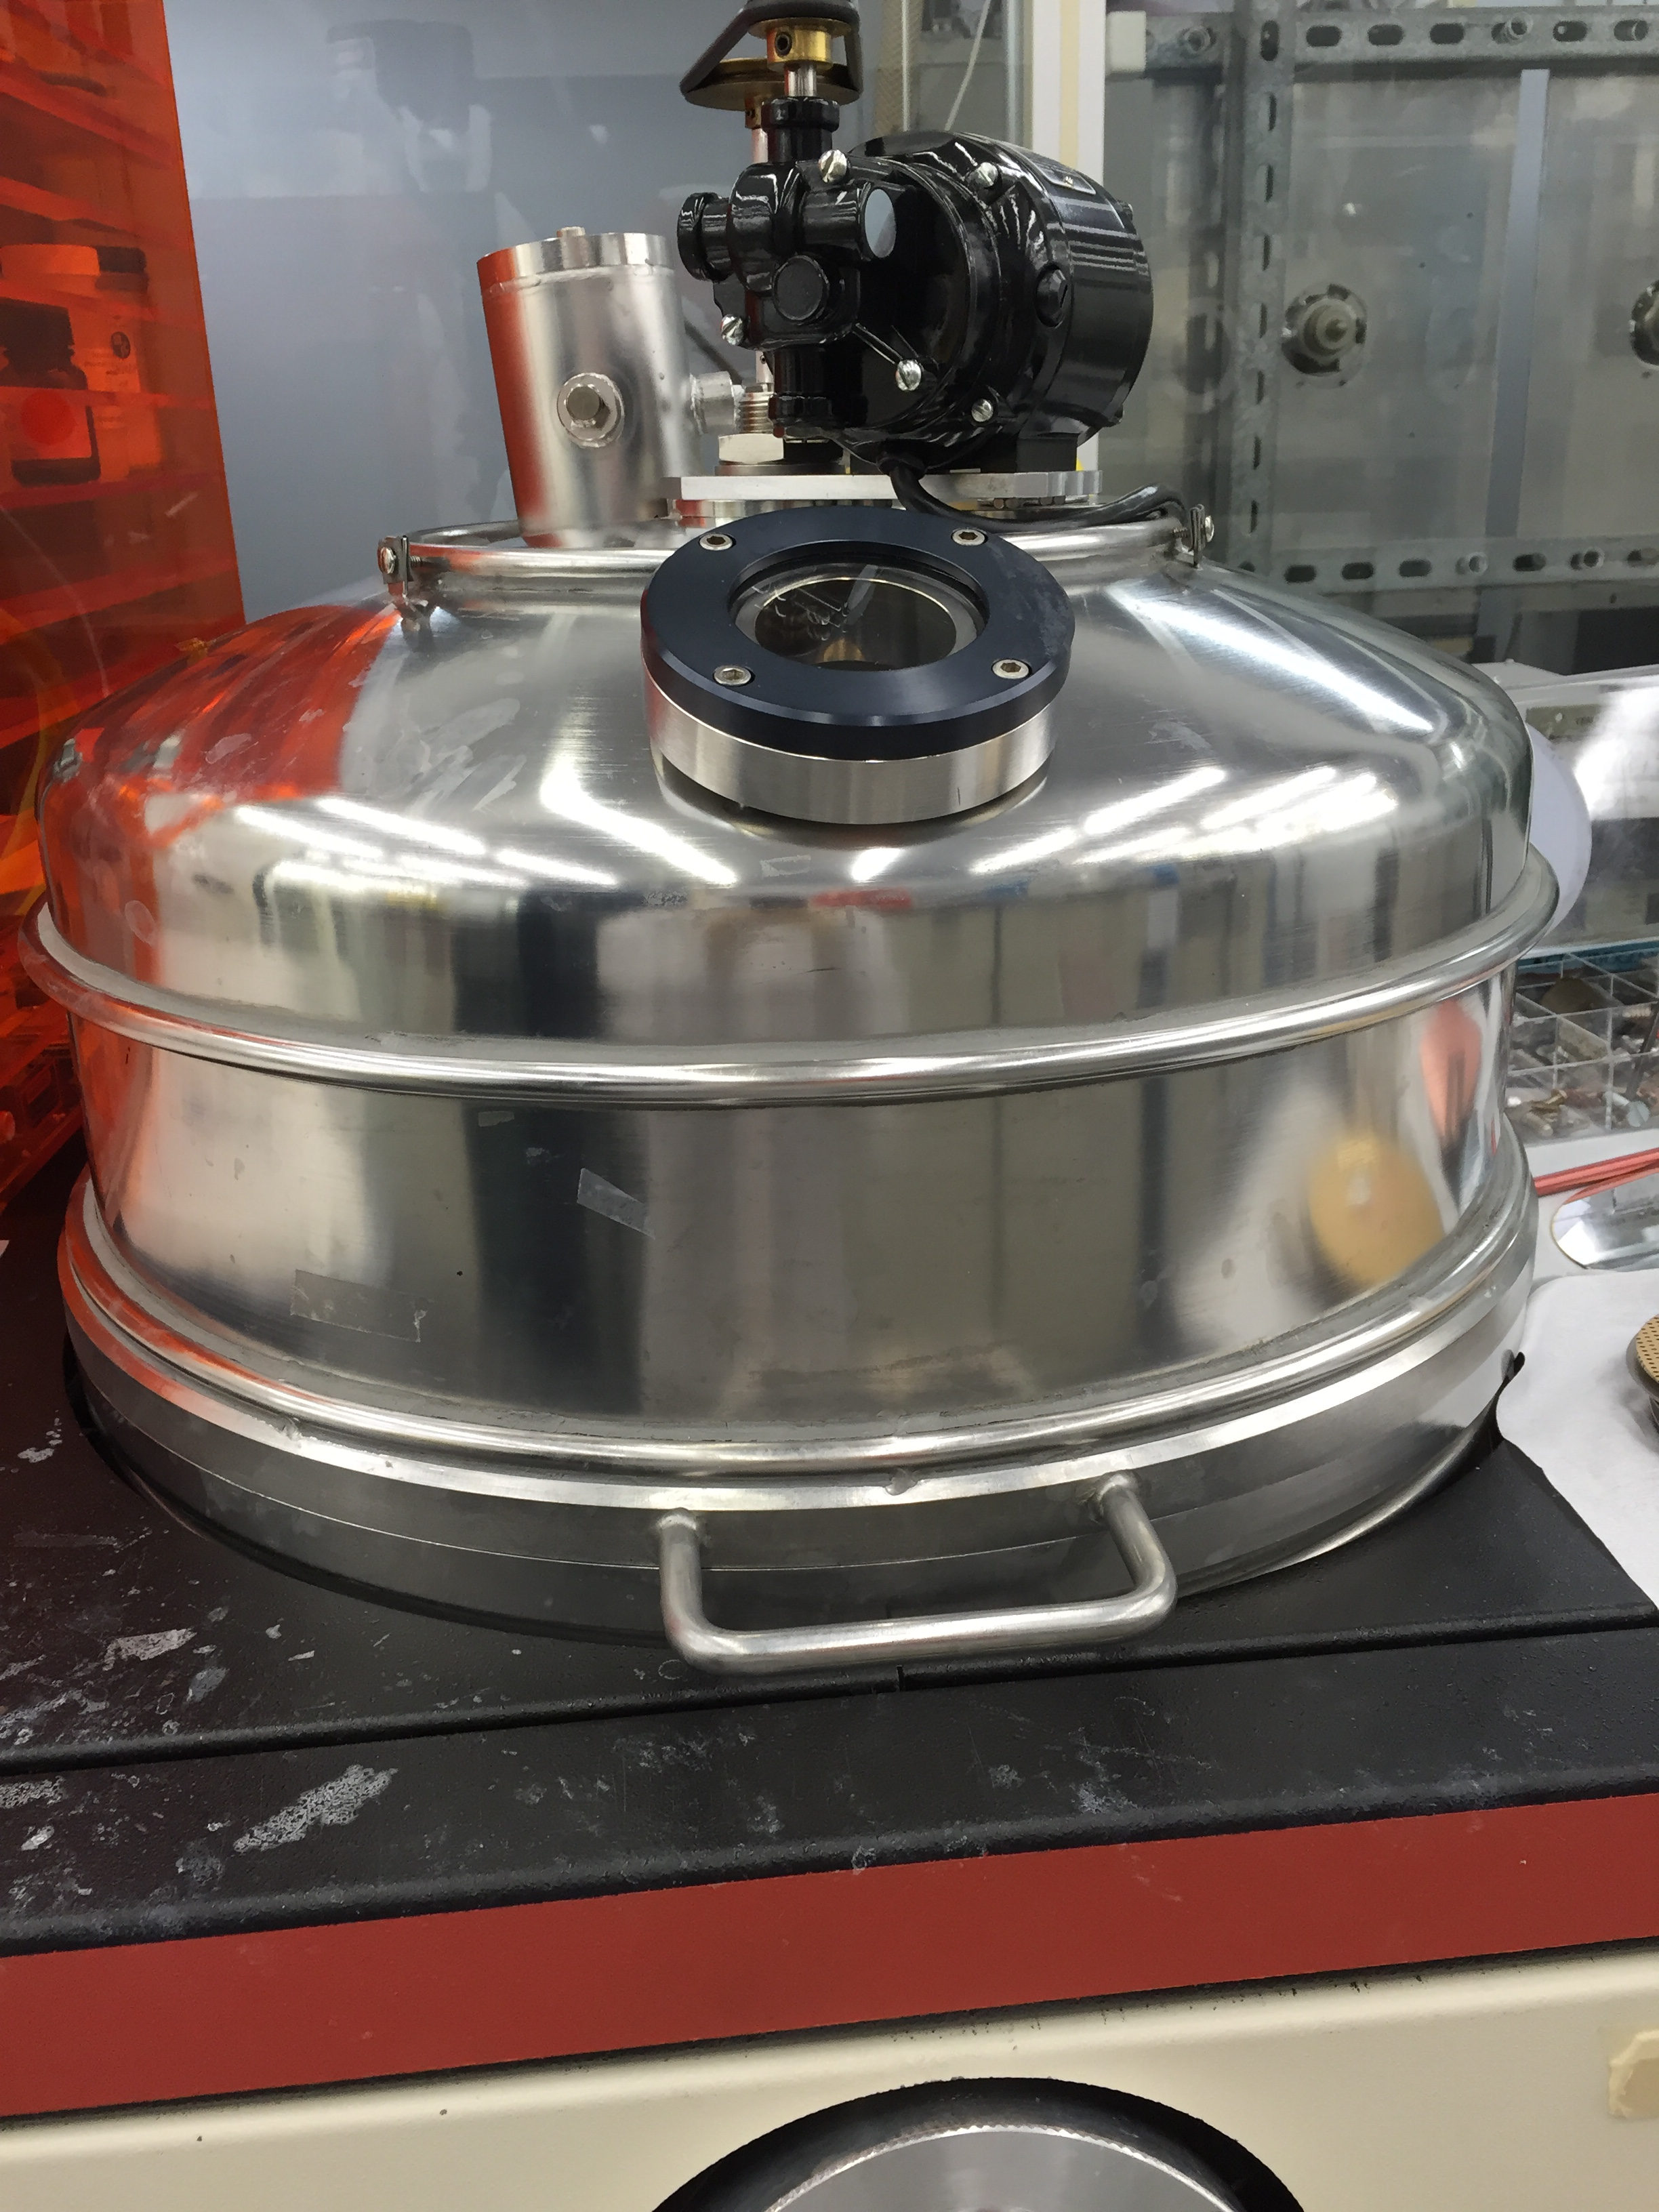
\includegraphics[height=4cm,width=4cm]{figs/experimental/bjd_hood}
		\caption[BJD Hood]{caption 2}
		\label{fig:bjd_hood}
	\end{minipage}
\end{figure}

\begin{figure}[ht]
	\centering
	\subfloat[\ch{Au}/\ch{Ti} deposited on developed sample after electron beam lithography at 10x]{
		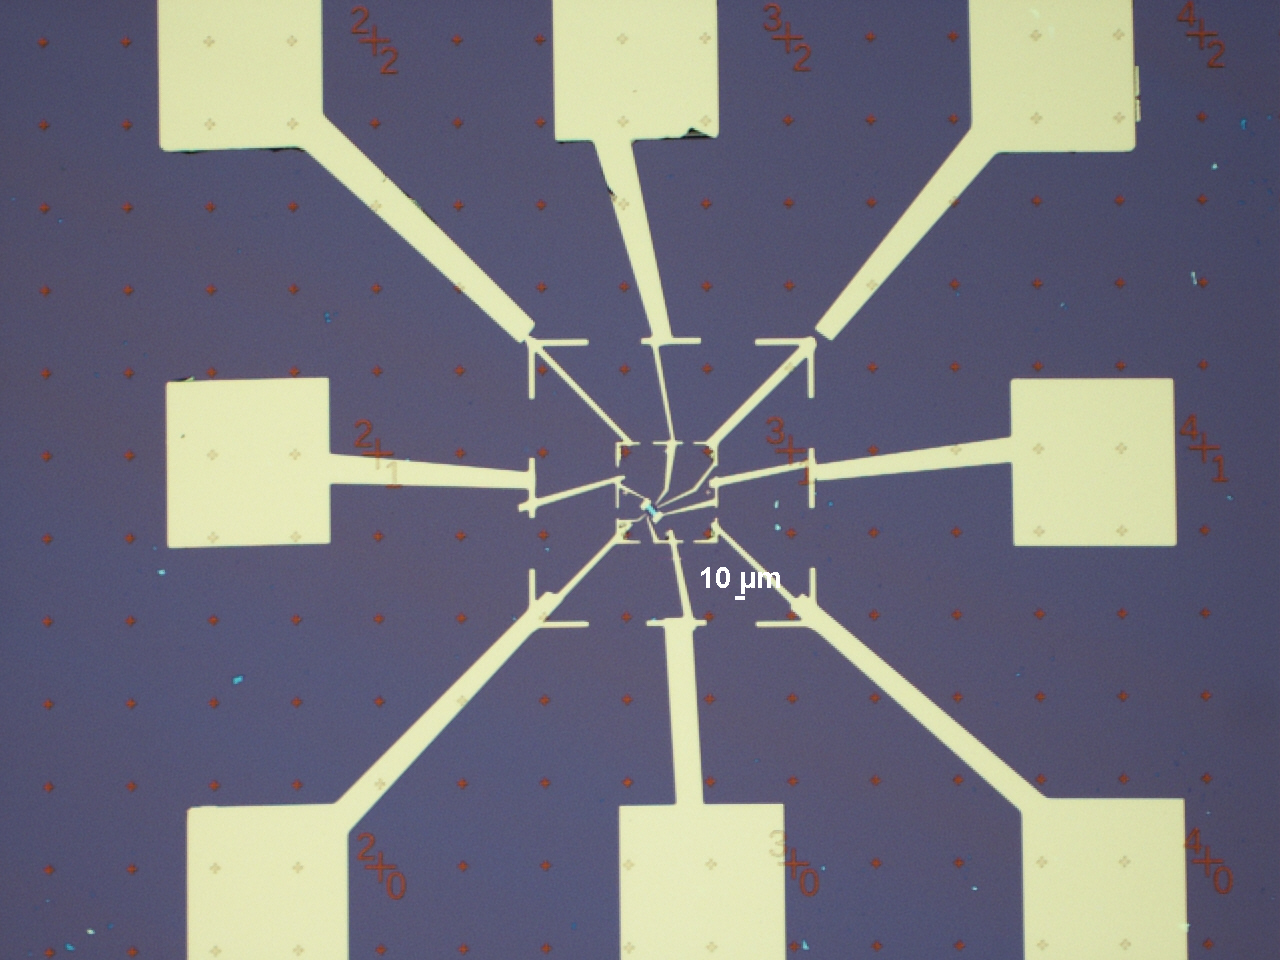
\includegraphics[height=4cm,width=4cm]{figs/experimental/liftoff_10x}
		\label{fig:liftoff_10x}
	}
	\qquad
	\subfloat[\ch{Au}/\ch{Ti} deposited on developed sample after electron beam lithography at 100x]{
		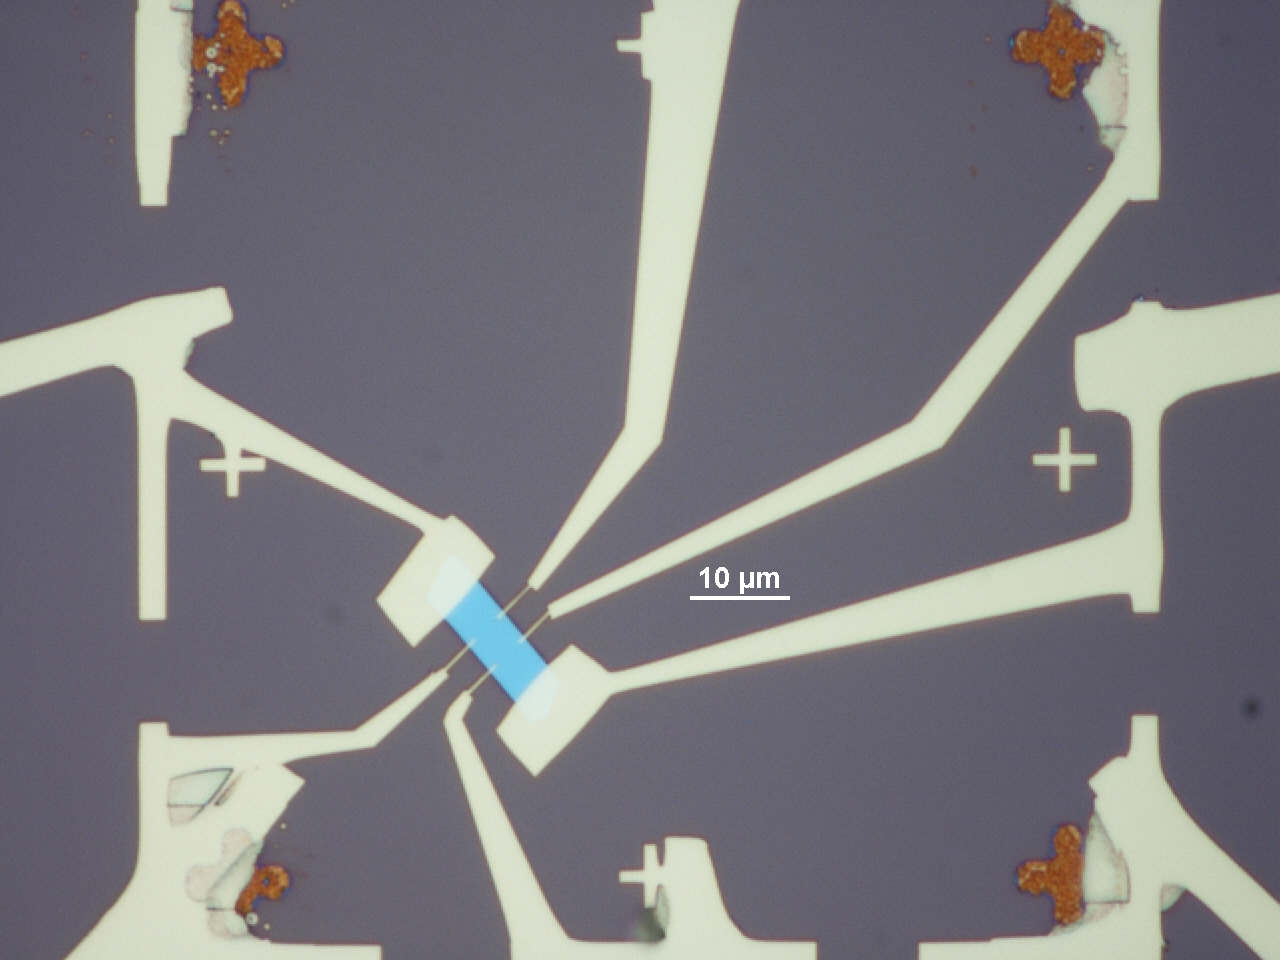
\includegraphics[height=4cm,width=4cm]{figs/experimental/liftoff_100x}
		\label{fig:liftoff_100x}
	}
	\caption[\ch{Au}/\ch{Ti} deposited on device]{Metal deposition on a device pattern.}
\end{figure}


\section{Electrical Measurements}\label{sec:measurements}
\subsection{Measurement Devices}\label{subsec:measurement_devices}
\begin{figure}[ht]
	\centering
	\subfloat[Keithley semiconductor measurement system]{
		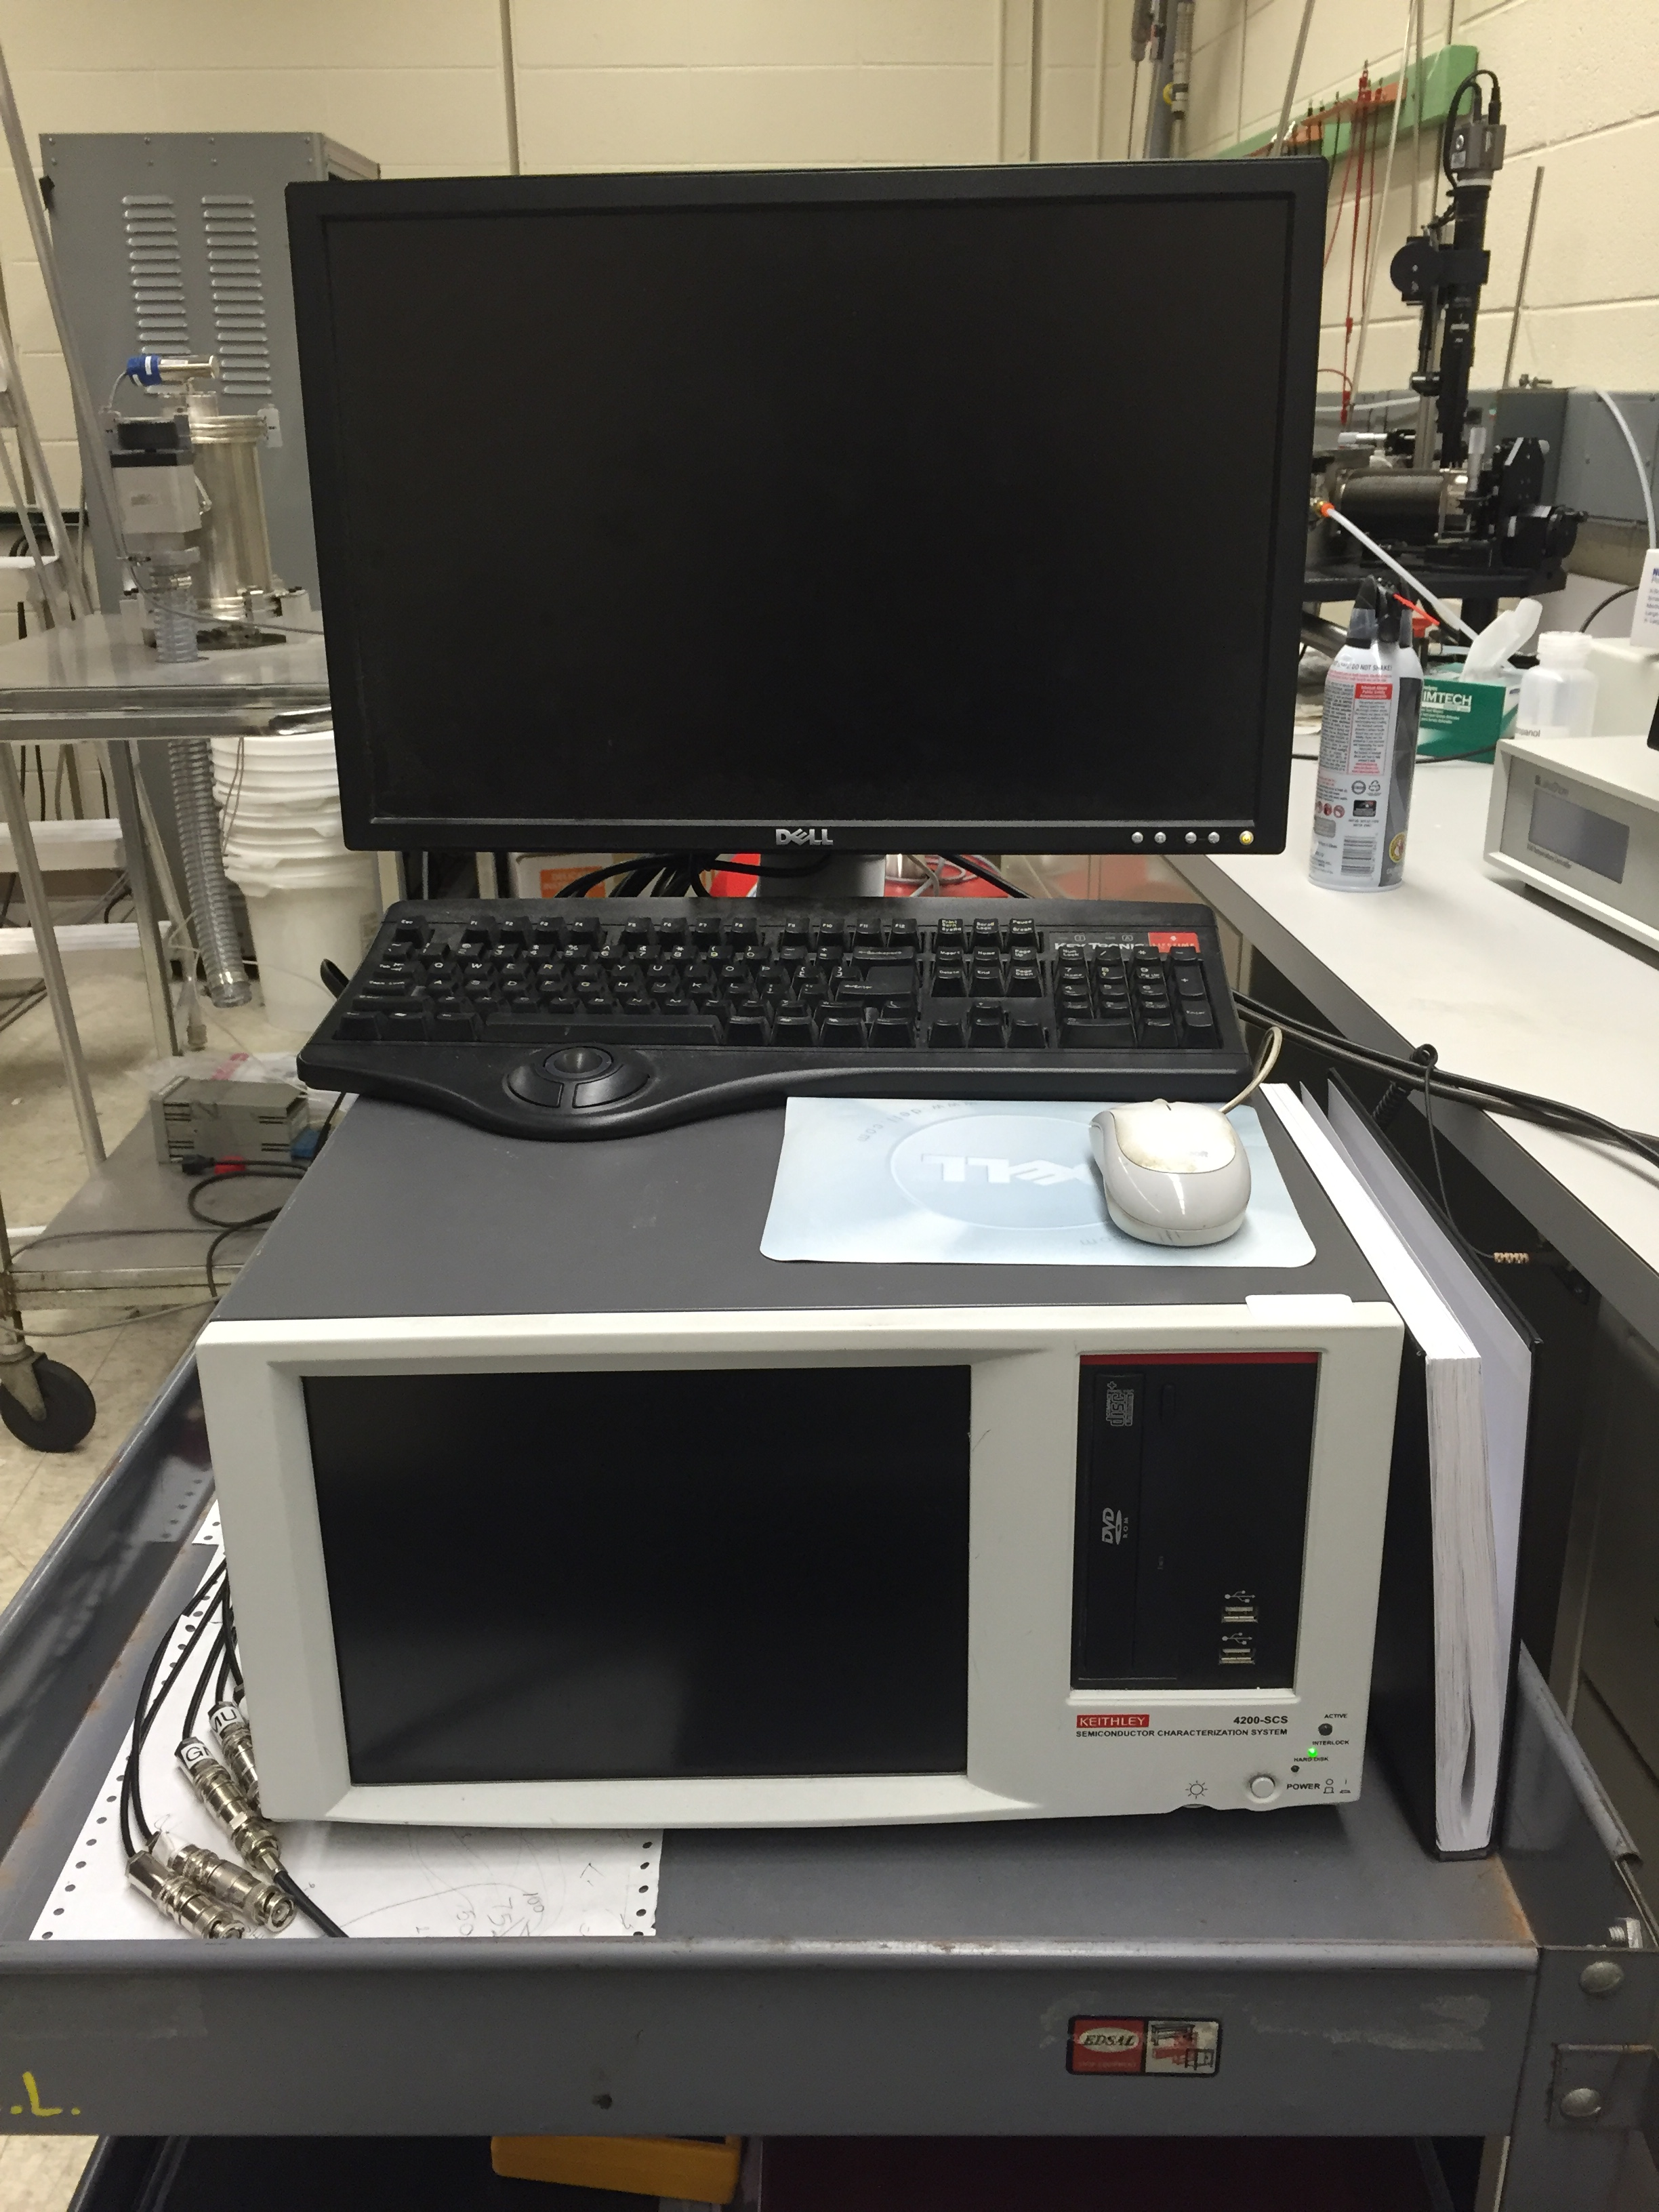
\includegraphics[height=4cm,width=4cm]{figs/experimental/measurement_setup}
		\label{fig:measurement_setup}
	}
	\qquad
	\subfloat[Low temperature, vacuum measurement chamber.]{
		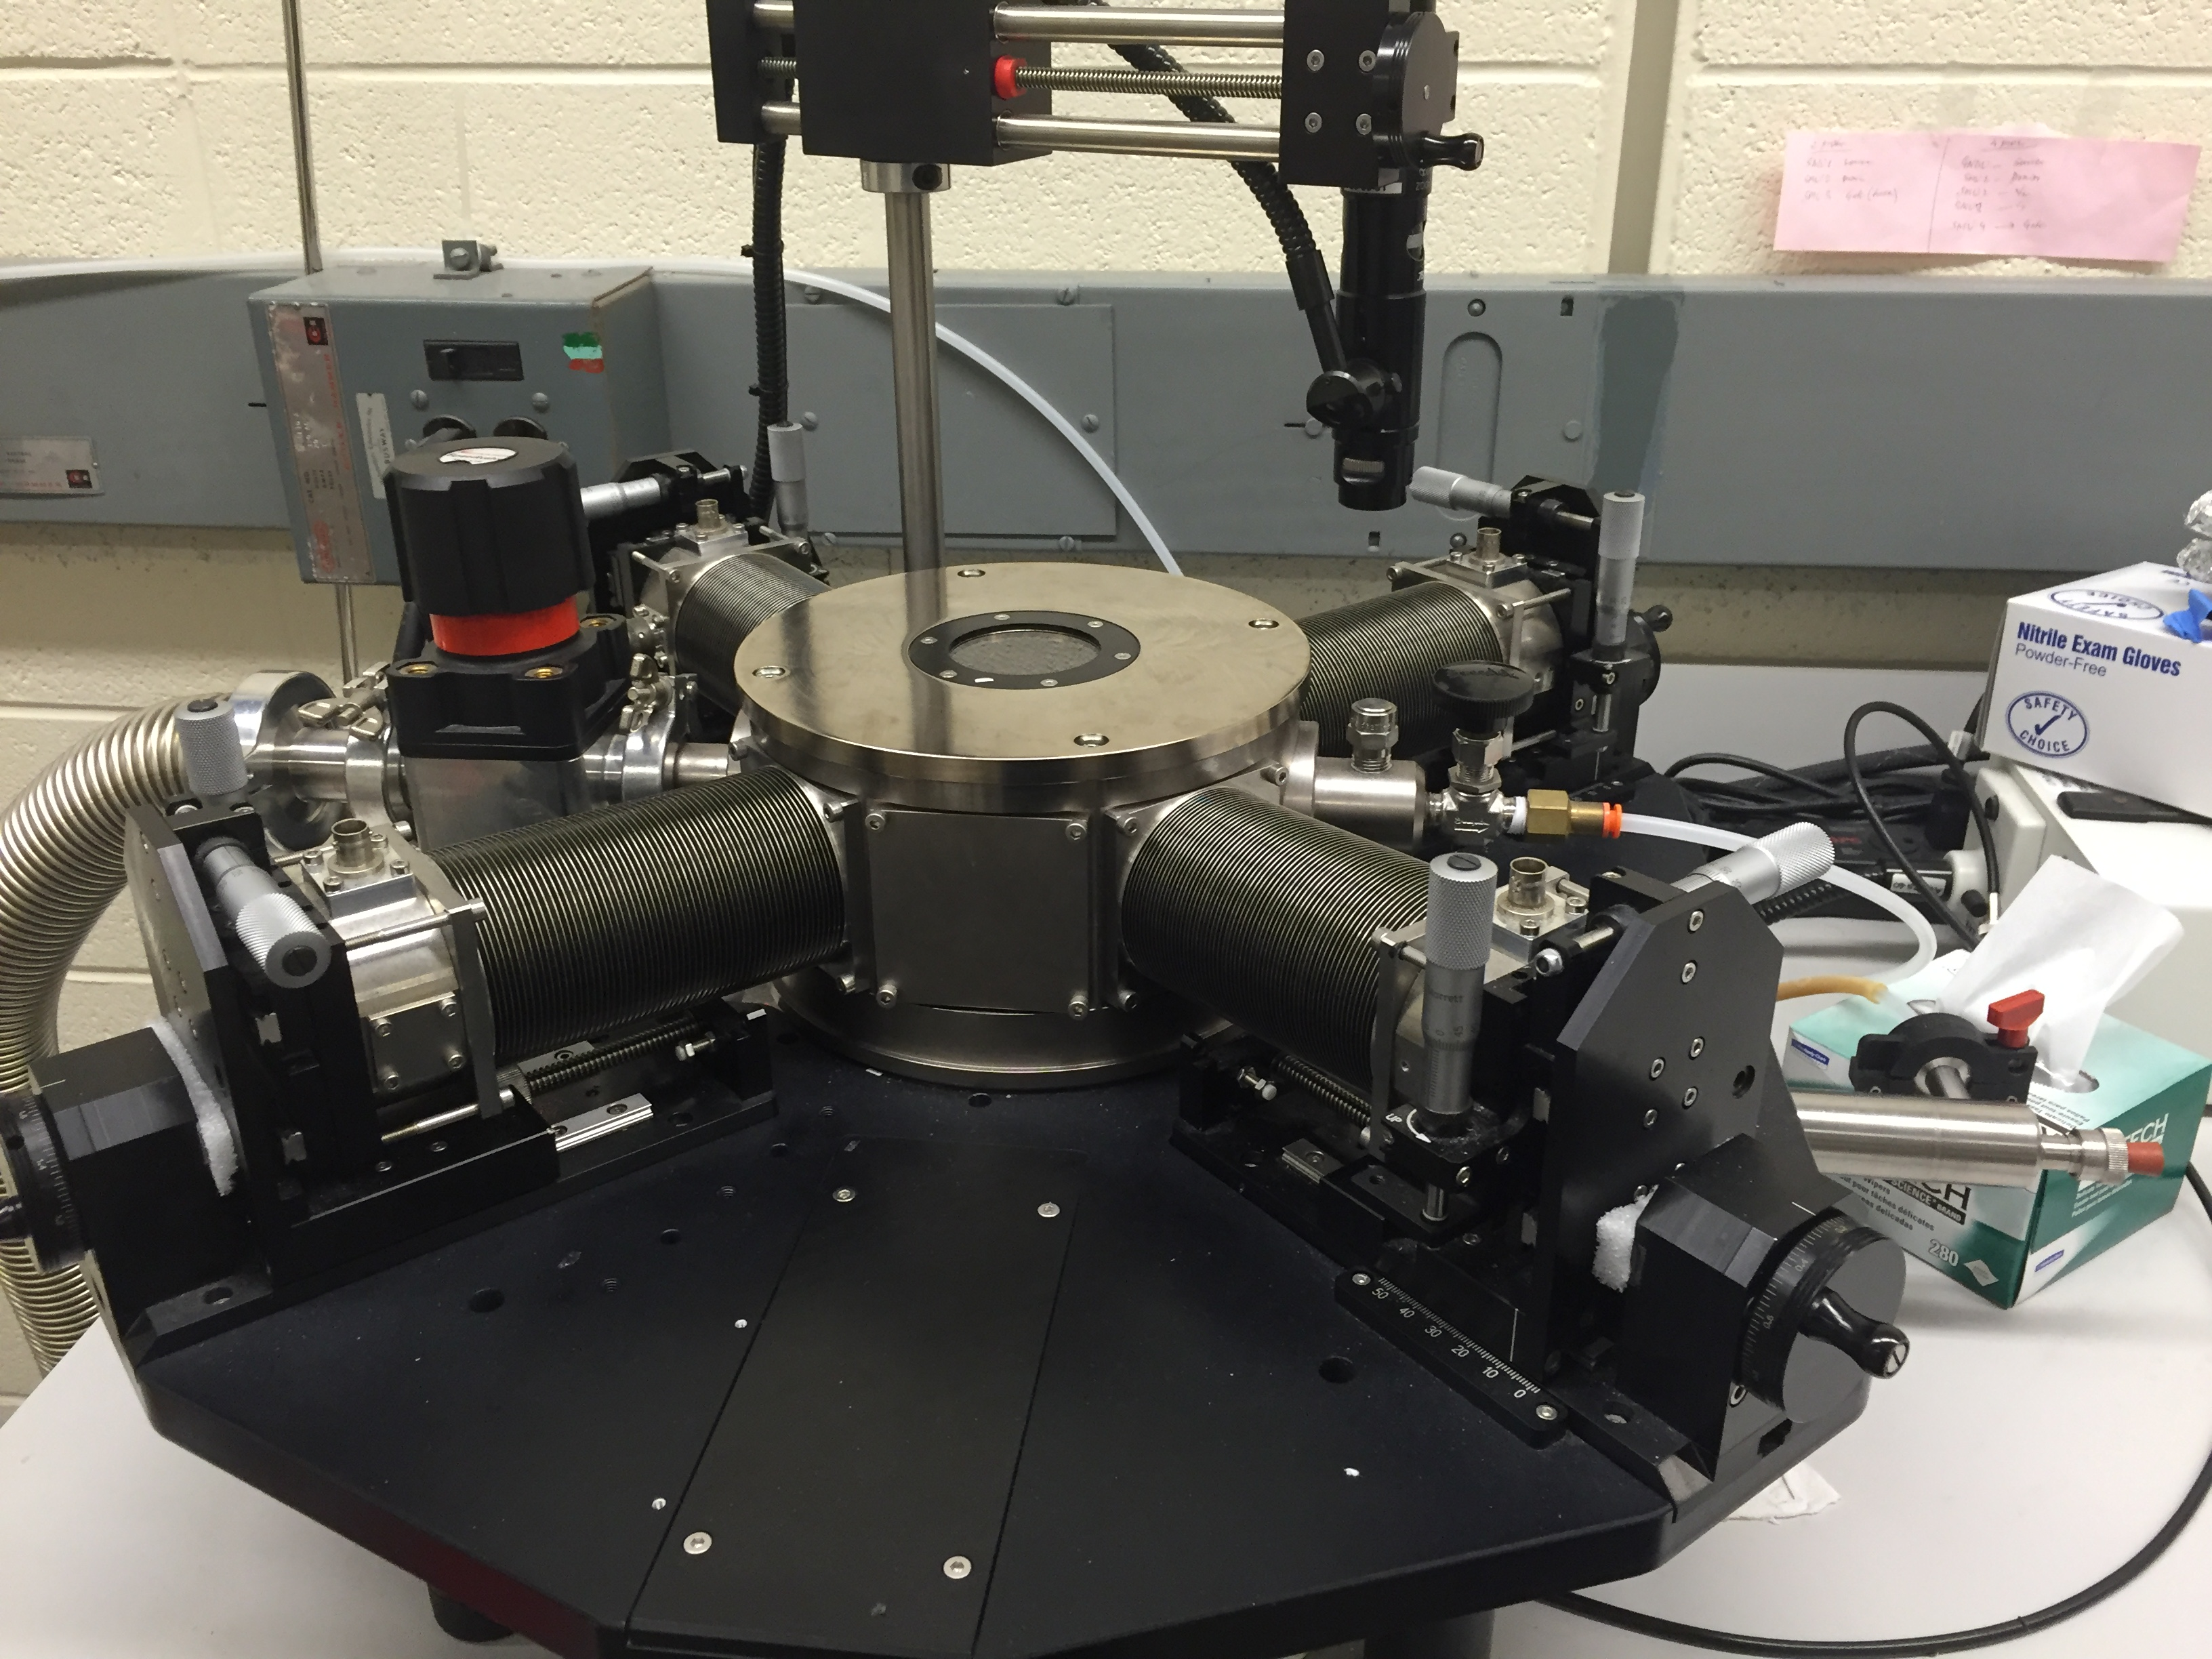
\includegraphics[height=4cm,width=4cm]{figs/experimental/vacuum_measurement}
		\label{fig:vacuum_measurement}
	}
	\caption[Measurement setup]{Main Caption}
	\label{fig:measurement}
\end{figure}

\begin{figure}[ht]
	\centering
	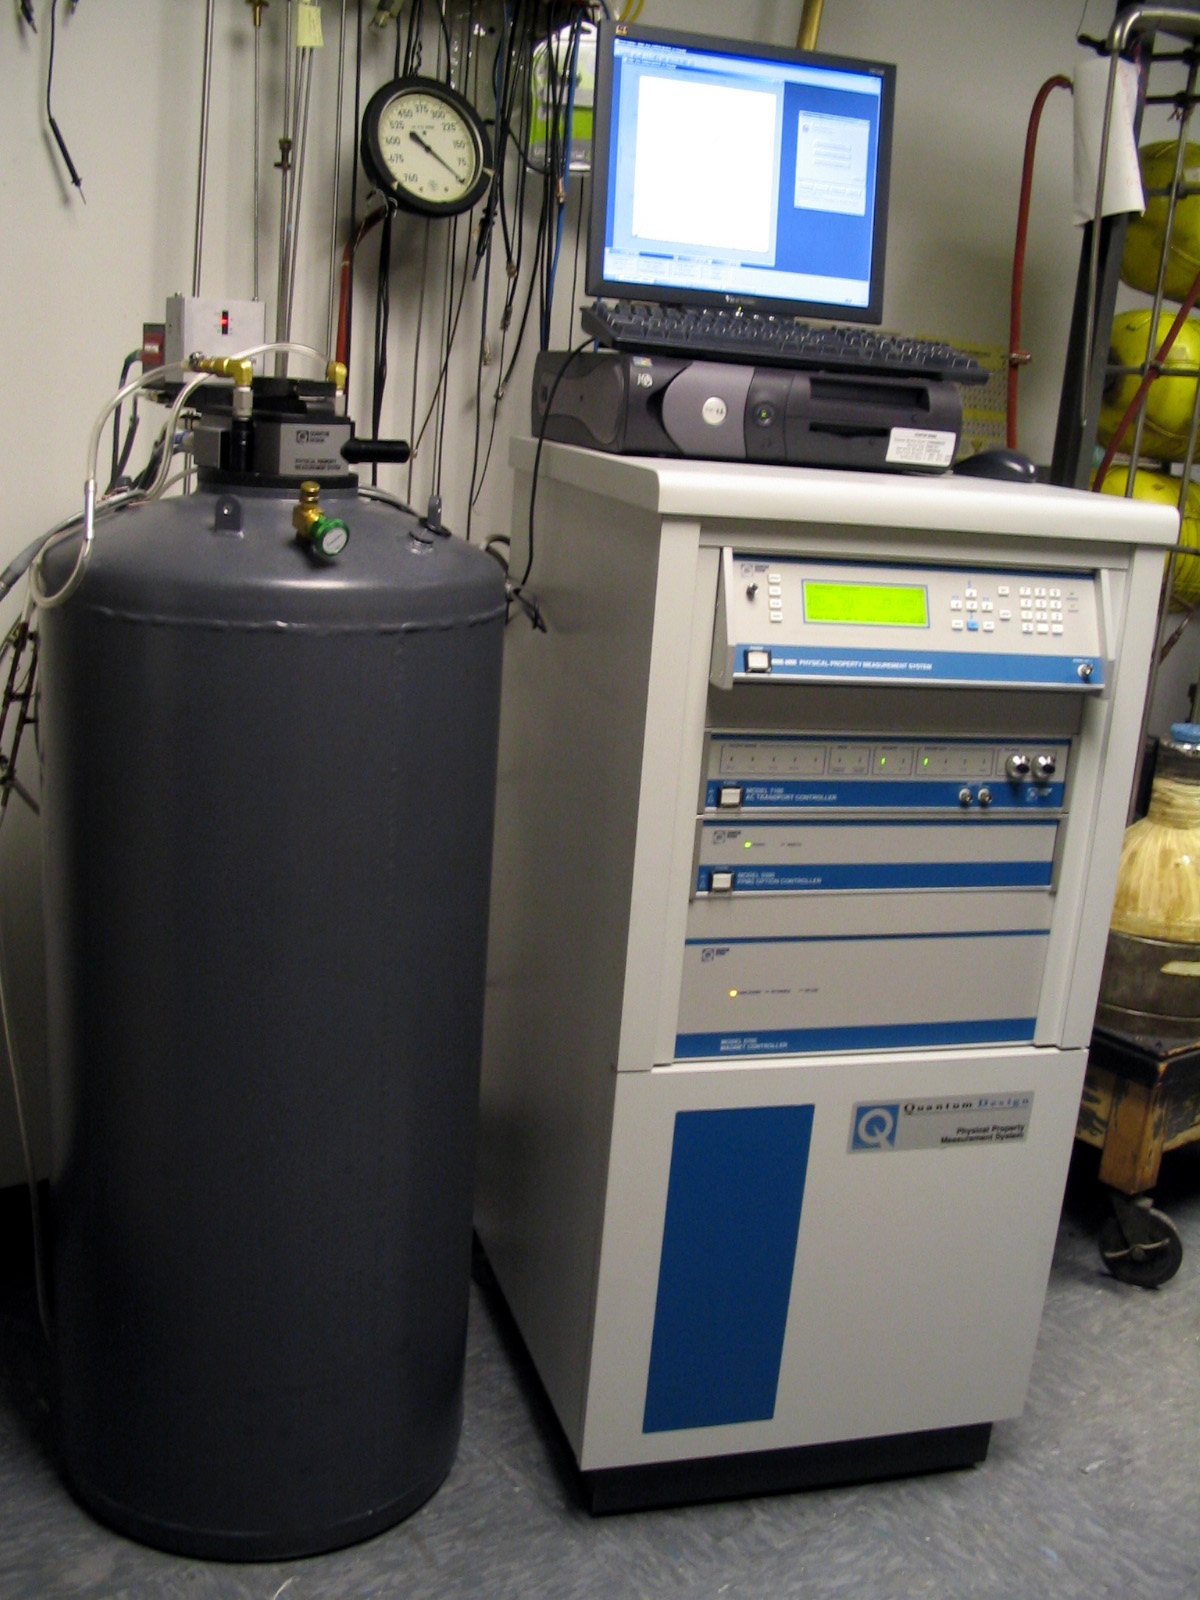
\includegraphics[height=4cm,width=4cm]{figs/experimental/ppms}
	\caption[Physical property measurement system]{\ac{PPMS} for measuring Hall effect and other transport properties.}
	\label{fig:ppms}
\end{figure}

 %!!!!!!!!!!!!!uncomment
	\chapter{Intrinsic Channel Properties and Scattering Mechanisms}\label{chap:results}
Developing low resistance two-dimensional/two-dimensional (2D/2D) ohmic contacts opens up possibility to study the intrinsic properties of \acp{TMD} and quantum physics. In particular, quantum phenomena inherent to \acp{2DEG} and \acp{2DHG} such as the \ac{IQHE} and \ac{SdH} oscillations can be explored in high mobility monolayer and few-layer \acp{TMD} \cite{Cui_NatureNano2015}. In addition to quantum transport properties and quantum effects in monolayer and few-layer \acp{TMD} the study of mobility and its corresponding temperature dependence can be used to understand the multiple scattering mechanisms present \cite{Kaasbjerg_PhysRevB2012}. These study of both electron and hole transport mechanisms is important due to the fact that high-performance $p$-type and $n$-type transistors are necessary for complimentary digital applications. 

\section{$p$-type \ch{WSe2} Semiconductor Contact Resistance}\label{sec:pWSe2_contacts}
One of the major challenges that still remains in fabricating devices to study intrinsic channel properties and scattering mechanisms is developing high quality $p$-type \ch{WSe2} devices. This is due to the fact that the metal/\ch{WSe2} (or \ch{MoS2}) interface is obstructed by a large \ac{SB} formed by the Fermi level pinning close to the conduction band of the \ch{WSe2} \cite{Chuang_NanoLett2014,Das_NanoLett2012}. \\ \\

\noindent In order to fabricate high quality $p$-type \ch{WSe2} devices, one aspect that must be addressed is how doping affects the \ac{SBH}. In particular, it is important to determine how doping can improve the 2D/2D contacts in devices. To address this issue of contact resistance several devices were fabricated and characterized in order to determine the contact resistance. Using the \ac{TLM} several \ch{WSe2} devices were made with electrodes spaced at varying lengths from the source electrode. 
\begin{figure}[ht]
	\centering
	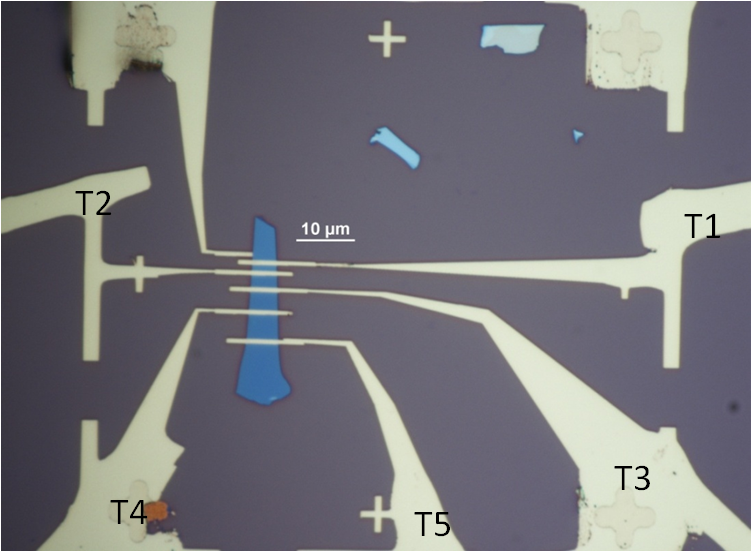
\includegraphics[height=5cm,width=7cm]{figs/results/transmission_line/transmission_device_pic_5-5_21_10232015_no1}
	\caption[Transmission line $0.05\%$ \ch{Nb} doped \ch{WSe2} channel device]{$0.05\%$ \ch{Nb} doped \ch{WSe2} channel transmission lines with corresponding channel lengths and widths of $L_{12} = 1.04\unita{\mu m}$ $W_{12} = 4.42\unita{\mu m}$, $L_{23} = 2.04\unita{\mu m}$, $W_{23} = 4.47\unita{\mu m}$, $L_{34} = 3.09\unita{\mu m}$, $W_{34} = 4.90\unita{\mu m}$, $W_{45} = 5.15\unita{\mu m}$, and $L_{45} = 4.27\unita{\mu m}$.}
	\label{fig:transmission_device_10232015_no1}
\end{figure}
Fig.~\ref{fig:transmission_device_10232015_no1} illustrates an example of a transmission line device that was used to characterize the contact resistance. The device shown has a $0.05\%$ \ch{Nb} doped \ch{WSe2} channel. The resistance in general is given by
\begin{equation}\label{eq:resistance_formula}
	R = \frac{\rho}{A} l,
\end{equation}
where, in this case, it is assumed that the resistivity $\rho$ and the area $A$ are constant throughout the device \cite{Schroder_Semiconductor2006}. The resistance $R$ is then proportional to the length $l$. By determining the resistance as a function of length one can determine the contact resistance of the device. The total resistance of the device is given by
\begin{equation}\label{eq:resistance_total}
	R = R_\mathrm{c} + R_\mathrm{ch},
\end{equation}
where $R_\mathrm{c}$ and $R_\mathrm{ch}$ are the contact and channel resistances, respectively \cite{Schroder_Semiconductor2006}. Thus by finding the resistance from the gradient of an I-V characteristic curve, one can apply the logic from eqs.~\ref{eq:resistance_formula} and \ref{eq:resistance_total} to find the contact resistance.
\begin{figure}[ht]
	\centering
	\subfloat[]{
		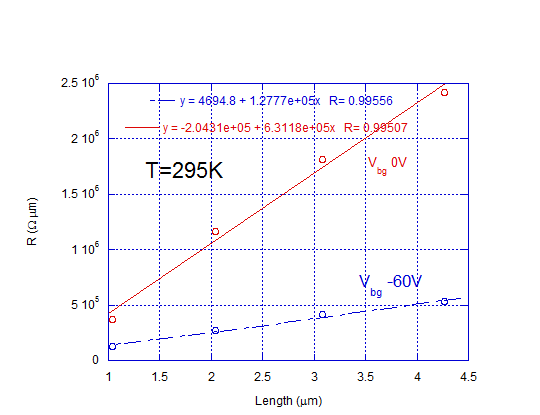
\includegraphics[height=3.5cm,width=4.25cm]{figs/results/transmission_line/transmission_resistance_plot_pic_5-5_21_10232015_no1}
		\label{fig:tlm_resistance1}
	}
	\qquad
	\subfloat[]{
		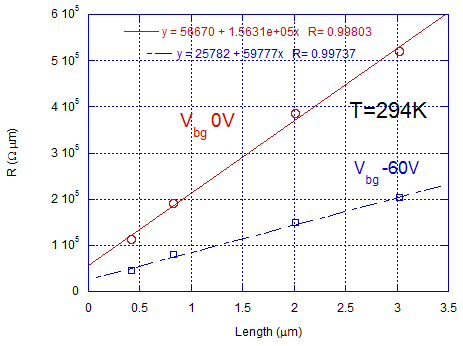
\includegraphics[height=3.5cm,width=4.25cm]{figs/results/transmission_line/transmission_resistance_plot_pic_56_21_10232015_no2}
		\label{fig:tlm_resistance2}
	}
	\qquad
	\subfloat[]{
		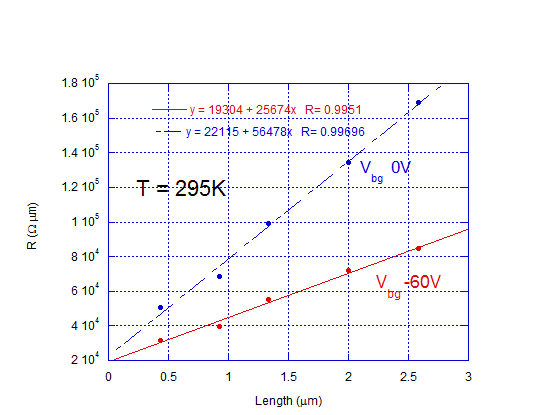
\includegraphics[height=3.5cm,width=4.25cm]{figs/results/transmission_line/transmission_resistance_plot_pic_-66_21_11182015_no2}
		\label{fig:tlm_resistance3}
	}
	\caption[Contact resistance of $0.05\%$ \ch{Nb} doped \ch{WSe2} channel device]{\protect\subref{fig:tlm_resistance1}-\protect\subref{fig:tlm_resistance3} show the resistance $R (\unita{\Omega\cdot\mu m})$ as a function of $L$, where the contact resistance is found by using a linear fit function. The fits were performed at $T=295\unita{K}$ for $V_{bg}$ of $0\unita{V}$ and $-60\unita{V}$. Note that \protect\subref{fig:tlm_resistance1} refers to the device shown in fig.~\ref{fig:transmission_device_10232015_no1}.}
	\label{fig:tlm_reistance_measurement}
\end{figure}
Using this method the resistance as a function of length is shown in figs.~\subref*{fig:tlm_resistance1}, \subref*{fig:tlm_resistance2}, and \subref*{fig:tlm_resistance3} for both $V_{bg}=0\unita{V}$ and $V_{bg}=-60\unita{V}$. From these figures one can interpret the contact resistance of the device as the intercept value with the value, the resulting contact resistances are summarized in table~\ref{table:contact_summary}. The results show linear behavior at room temperature for both backgate voltage of $V_{bg}=0\unita{V}$ and $V_{bg}=-60\unita{V}$. The reported resistance values are larger for lower $V_{bg}$ measurements, this can be explained by the energy mismatch of Fermi levels between the metal contacts and the lightly doped \ch{WSe2}. As the backgate voltage is increased from $V_{bg} = 0\unita{V}$ to $-60\unita{V}$ the \acs{SB} that is present in the contacts has narrowed and as a result of the increased $V_{bg}$ there is more transport across the barrier. The relatively small contact resistance of $2.35\unita{k\Omega\cdot\mu m}$ indicates that low resistance contacts can be achieved at sufficiently high backgate voltage. The contact resistances are on the same order of magnitude measured by Cui \emph{et al.} at $T=300\unita{K}$ and a relatively high backgate voltage ($~10\unita{\Omega\cdot\mu m}$) \cite{Cui_NatureNano2015}.  \\ \\

In light of this result, the addition of degenerately doped contacts (like those fabricated in sec.~\ref{sec:pWSe2_hbn}) could further improve the contact resistance. By adding $0.5\%$ \ch{Nb} doped \ch{WSe2} contacts, for example, the Fermi level energy mismatch between the metal and the degenerately doped \ch{WSe2} contact would be decreased. Thereby lowering the \acs{SBH} and coupled with sufficiently high backgate voltage, the ability to achieve $< 2\unita{k\Omega\cdot\mu m}$ contact resistance is plausible. 
\begin{table}[ht]
	\centering
	\begin{threeparttable}
		\begin{tabular}{c c c c}
			\hline\hline
			$L_\mathrm{min}$ & $L_\mathrm{max}$ & $R_\mathrm{c}(\unita{k\Omega\cdot\mu m})$ at $V_{bg}=0\unita{V}$ & $R_\mathrm{c}(\unita{k\Omega\cdot\mu m})$ at $V_{bg}=-60\unita{V}$ \\ [0.5ex]
			\hline
			$1.04\unita{\mu m}$ & $4.27\unita{\mu m}$ & $102$\tnote{a} & $2.35$\tnote{a}\\
			$0.42\unita{\mu m}$ & $3.02\unita{\mu m}$ & $28.4$\tnote{b} & $12.9$\tnote{b}\\
			$0.43\unita{\mu m}$ & $2.58\unita{\mu m}$ & $11.1$\tnote{c} & $9.65$\tnote{c}\\ [1ex]
			\hline
		\end{tabular}
		\begin{tablenotes}
			\item[a] Length and resistance values from fig.~\subref*{fig:tlm_resistance1}.
			\item[b] Length and resistance values from fig.~\subref*{fig:tlm_resistance2}.
			\item[c] Length and resistance values from fig.~\subref*{fig:tlm_resistance3}.
		\end{tablenotes}
	\caption[Summary of contact resistances for $0.05\%$ \ch{Nb} doped \ch{WSe2} channel]{Summary of contact resistances for $0.05\%$ \ch{Nb} doped \ch{WSe2} channel found using linear fit data from figs.~\ref{fig:tlm_resistance1}, \ref{fig:tlm_resistance2}, and \ref{fig:tlm_resistance3}.}
	\label{table:contact_summary}
	\end{threeparttable}
\end{table}

\section{$p$-type \ch{WSe2} Hall Effect Measurements}\label{sec:pWSe2_hall}
In addition to knowing the how doping can be used to lower the \acs{SBH}, doping also affects the intrinsic channel properties. To study how these properties are effected several measurements were taken. First, Hall bar devices were fabricated. These devices were similar to those used in sec.~\ref{sec:pWSe2_contacts}, the channel was doped with the same amount of \ch{Nb}. The only differing aspect of these devices was the electrode design. Fig.~\subref*{fig:hall_bar_device1} shows an example of one such Hall bar device. \\ \\

\noindent The Hall effect measurement is widely used for semiconductor characterization as it gives useful electrical properties such as the resistivity, carrier density, and mobility \cite{Schroder_Semiconductor2006}. Consider the setup shown in fig.~\ref{fig:hall_diagram}, where the length $L$ is taken in the $x$-direction, width $w$ in the $y$-direction, thickness $t$ in the $z$ direction, and $e$ denotes a charge carrier which can be either an electron or a hole. The current $I$ flows in the positive $x$-direction and is given by 
\begin{equation}\label{eq:hall_current}
	I = J w t = n e v_x w t,
\end{equation}
where $J$ is the current density in the $x$-direction, $n$ is the charge carrier number density, and $v_x$ is the charge carrier drift velocity in the positive $x$-direction. The current $I$ is a result of the application of an electric field $E$ along the positive $x$-direction. In the presence of a magnetic field $B$ in the positive $z$ direction the charge carriers will experience a Lorentz force that deflects them toward one side of the device. As a result there is an accumulation of charges alone one side of the device which in turn creates a transverse electric field $E_y$ \cite{Melissinos_Experiments1966}. The transverse electric field $E_y$ is given by
\begin{equation}\label{eq:Ey}
	E_y = v_x B,
\end{equation}
where $B$ is the magnetic field in the $z$ direction. This accumulation of charges along one side of the device creates a potential difference that is related to the transverse electric field $E_y$ and can easily be used to find the Hall voltage $V_H$ by
\begin{equation}\label{eq:hall_voltage}
	V_H = -\int_0^w E_y\,dy = - E_y w.
\end{equation}
Finally, by combining eqs.~\ref{eq:hall_current}, \ref{eq:Ey}, and \ref{eq:hall_voltage} a final expression for the Hall voltage $V_H$ is given by
\begin{equation}\label{eq:hall_voltage_final}
	V_H = -\frac{I B}{t}\left(\frac{1}{ne}\right).
\end{equation}
From eq.~\ref{eq:hall_voltage_final} two forms of the Hall coefficient become evident,
\begin{equation}\label{eq:RH}
	R_H = \frac{1}{ne} = \frac{V_H t}{I B}.
\end{equation}
Since $e$ refers to either holes or electrons, the sign of $R_H$ would also vary in accord with the proper carrier being described in the circumstance. Furthermore the conductivity is given by 
\begin{equation}\label{eq:hall_conduct}
	\sigma = n e \mu_H,
\end{equation}
where $\sigma$ is the conductivity and $\mu_H$ denotes the Hall mobility. Thus, an expression for the Hall mobility can be found by combining eqs.~\ref{eq:RH} and \ref{eq:hall_conduct} to give
\begin{equation}\label{eq:mu_H}
	\mu_H = \abs{R_H}\sigma = \frac{\sigma V_H t}{I B}.
\end{equation}
\begin{figure}[ht]
	\centering
	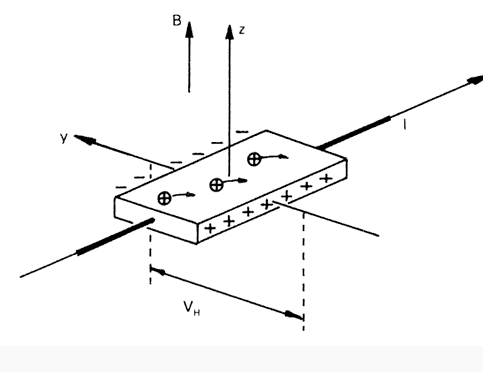
\includegraphics[height=6cm,width=8cm]{figs/results/hall_diagram}
	\caption[Hall effect measurement diagram]{Geometry of Hall effect measurement. Current flows in the positive $x$-direction and magnetic field is applied in the positive $z$ direction generating a Hall voltage \cite{HallEffectNIST}. Diagram originally appeared in ref.~\cite{HallDiagram}.}
	\label{fig:hall_diagram}
\end{figure}
\noindent Following this prescribed method to determine the Hall coefficient it was used to find the Hall mobility $\mu_H$ and charge carrier density for lightly doped channel \ch{WSe2} devices.
\begin{figure}[ht]
	\centering
	\subfloat[]{
		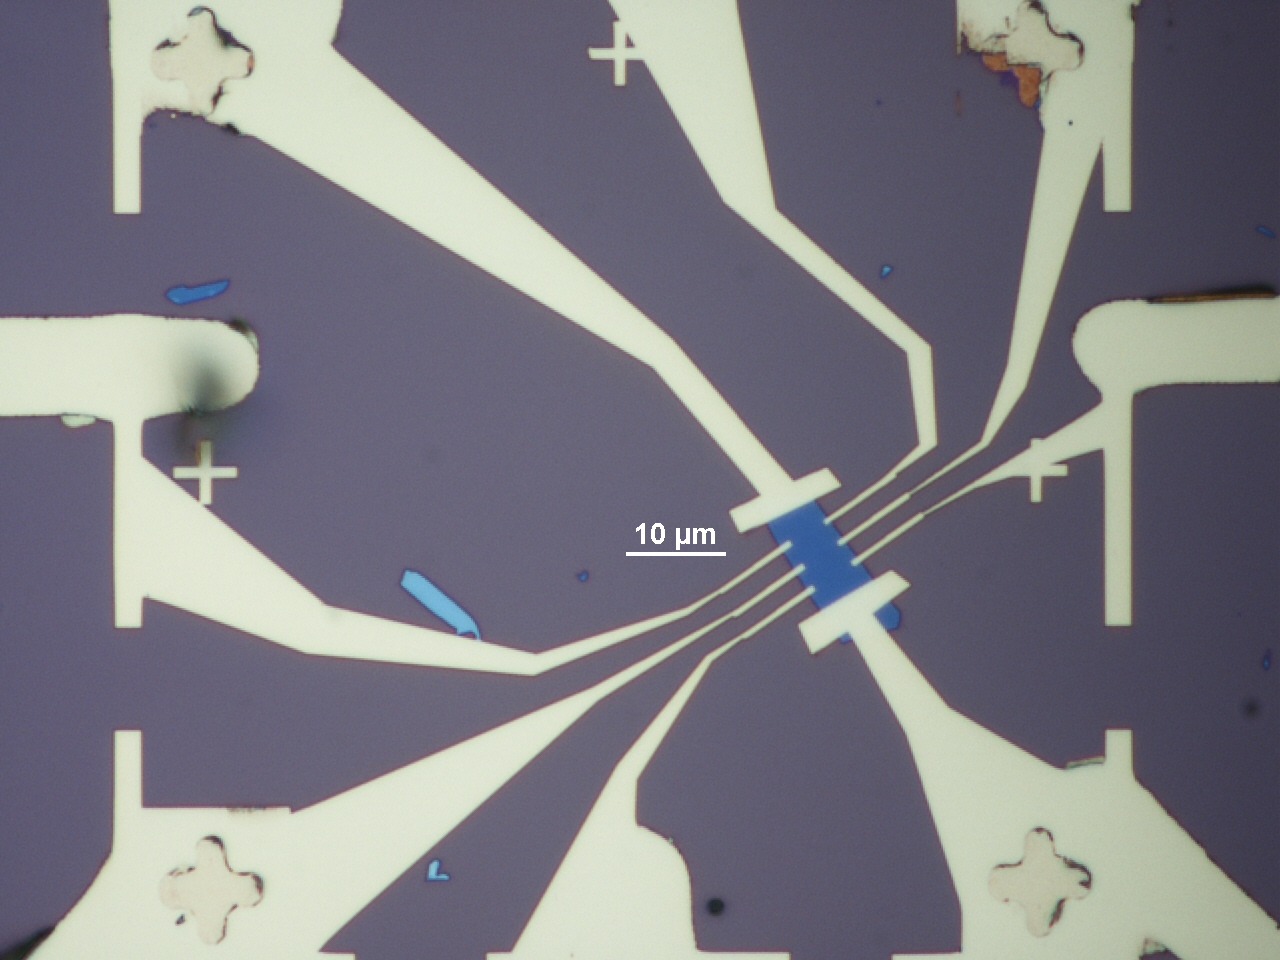
\includegraphics[height=3.5cm,width=4.25cm]{figs/results/hall_bar_doped_channel/hall_bar_device_pic_11192015_no1}
		\label{fig:hall_bar_device1}
	}
	\qquad
	\subfloat[]{
		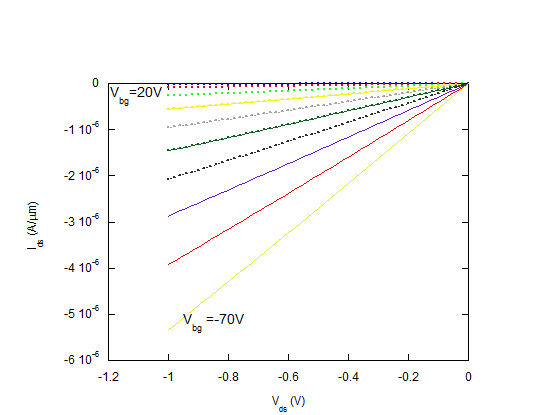
\includegraphics[height=3.5cm,width=4.25cm]{figs/results/hall_bar_doped_channel/Vds-Id_1V_-1V-Vbg_20V_-70V_T1-D_T5_S_300K_plot_modified_11192015_no2}
		\label{fig:11192015_ohmic_contacts}
	}
	\qquad
	\subfloat[]{
		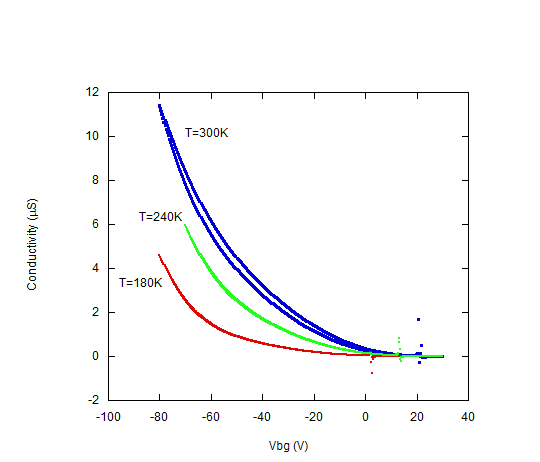
\includegraphics[height=3.5cm,width=4.25cm]{figs/results/hall_bar_doped_channel/hall_bar_device_pic_11192015_no1_conduct_vs_Vbg_all_temps}
		\label{fig:11192015_conduct_vs_temp}
	}
	%\qquad

	\subfloat[]{
		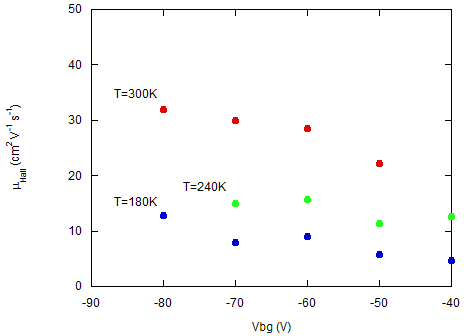
\includegraphics[height=3.5cm,width=4.25cm]{figs/results/hall_bar_doped_channel/hall_bar_device_pic_11192015_no1_mu_hall_vs_Vbg_all_temps}
		\label{fig:11192015_mu_hall_vs_temp}
	}
	\qquad
	\subfloat[]{
		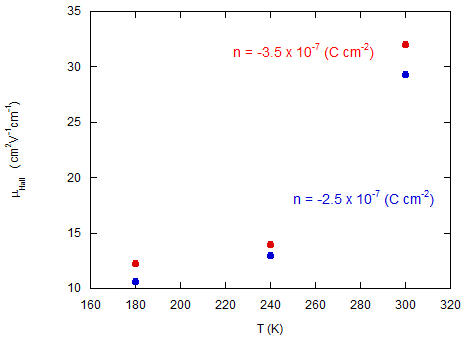
\includegraphics[height=3.5cm,width=4.25cm]{figs/results/hall_bar_doped_channel/HallMobility_Vs_T_for_fixed_carrier_consentrations_plot_modified_11192015_no2}
		\label{fig:11192015_mu_hall_vs_temp_various_n}
	}
	\qquad
	\subfloat[]{
		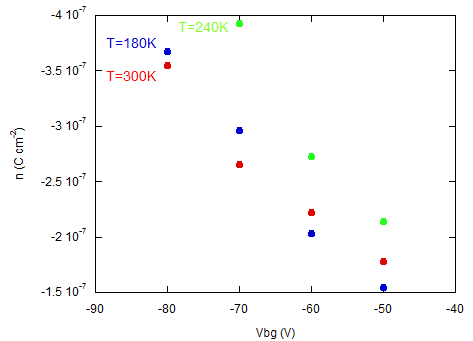
\includegraphics[height=3.5cm,width=4.25cm]{figs/results/hall_bar_doped_channel/Charge_density_Vs_Vbg_different_Temp_plot_modified_11192015_no1}
		\label{fig:11192015_n_vs_Vbg}
	}
	\caption[Hall measurement data for $0.05\%$ \ch{Nb} doped \ch{WSe2} channel]{\protect\subref{fig:hall_bar_device1} Hall bar device with $0.05\%$ \ch{Nb} doped \ch{WSe2} channel. Hall bar device with $0.05\%$ \ch{Nb} doped \ch{WSe2} channel. Sample thickness is $7.74\unita{nm}$ with an average width $W_\mathrm{avg}=5.74\unita{\mu m}$. \protect\subref{fig:11192015_ohmic_contacts} IV characteristic curves at $T=300K$ for $V_{bg}$ ranging from $-70\unita{V}$ to $20\unita{V}$. \protect\subref{fig:11192015_conduct_vs_temp} Conductivity as a function of $V_{bg}$ for various temperatures. \protect\subref{fig:11192015_mu_hall_vs_temp} Hall mobility as a function of $V_{bg}$ for various temperatures. \protect\subref{fig:11192015_mu_hall_vs_temp_various_n} Hall mobility as a function of temperature for different charge carrier densities. \protect\subref{fig:11192015_n_vs_Vbg} Charge carrier density as a function of $V_{bg}$ for various temperatures.}
	\label{fig:hall_measurement_data1}
\end{figure}

\noindent Fig.~\subref*{fig:11192015_ohmic_contacts} illustrates ohmic IV characteristics for the device pictured in fig.~\ref{fig:hall_bar_device1} for $V_{bg}$ ranging from $-70\unita{V}$ to $20\unita{V}$ at $T=300\unita{K}$. Fig.~\subref*{fig:11192015_conduct_vs_temp} shows the conductivity $\sigma$ as a function of $V_{bg}$ for various temperatures. As the temperature increases one notices that the conductivity also increases (WHY IS THIS TRUE?). In addition to the conductivity increasing with temperature, so too, does the Hall mobility $\mu_H$. This fact is shown in fig.~\subref*{fig:11192015_mu_hall_vs_temp}. The Hall mobility as a function of temperature for charge carrier densities $n=-3.5\times 10^{-7}\unita{C}\unitb{cm}{-2}$ and $n=-2.5\times 10^{-7}\unita{C}\unitb{cm}{-2}$ is shown in fig.~\subref*{fig:11192015_mu_hall_vs_temp_various_n}. Fig.~\subref*{fig:11192015_n_vs_Vbg} shows the charge carrier density $n$ as a function of $V_{bg}$ for several temperatures (DOES DATA MAKE SENSE?). 

\section{$p$-type \ch{WSe2} Field-Effect Mobility}\label{sec:pWSe2_hbn}
In an effort to improve on the approaches and results described in secs.~\ref{sec:pWSe2_contacts} and \ref{sec:pWSe2_hall} a new design of device was fabricated. These devices used a $0.01\%$ \ch{Nb} doped \ch{WSe2} (lightly doped)channel with $0.5\%$\ch{Nb} doped \ch{WSe2} (degenerately doped) contacts. The device fabrication process involved transferring \hbn to a \ch{Si}/\ch{SiO2} substrate then transferring the $p$-doped \ch{WSe2} on top of the bottom \hbn creating the channel (see fig.~\subref*{fig:pWSe2_doped_contacts_and_channel_step1_pt2}). Once the $p$-doped \ch{WSe2} is on the bottom \hbn substrate then another layer of \hbn is transferred to cover the channel (see fig.~\subref*{fig:pWSe2_doped_contacts_and_channel_step2_pt2}). Next, the degenerately doped \ch{WSe2} contacts are transferred onto the device (see fig.~\subref*{fig:pWSe2_doped_contacts_and_channel_step3_pt2}). Finally, the electrodes are designed and the usual device fabrication steps ensue, fig.~\subref*{fig:pWSe2_doped_contacts_and_channel_final_device_pt2} shows an example of a measurement-ready device. The main quantity of interest here is the field-effect mobility as it allows for analysis of the device`s quality and also allows for a determination of the possible scattering mechanisms present. The two-probe field-effect mobility is given by 
\begin{equation}\label{eq:mu_fe}
	\mu_\mathrm{FE} = \frac{L}{w}\frac{d I_{ds}}{d V_{bg}}\frac{1}{C}\frac{1}{V_{ds}},
\end{equation}
where $L$ is the length of the channel, $w$ is the width of the channel, $I_{ds}$ is the drain current, $V_{bg}$ is the backgate voltage, $C$ is the capacitence, and $V_{ds}$ is the drain voltage \cite{Stassen_AppPhysLett2004}. The capacitence is dependent largely on the substrate used, generally \ch{Si}/\ch{SiO2} and can vary from substrate to substrate as a result the field-effect mobility can vary slightly depending on the capacitence of the substrate.  \\ \\
\begin{figure}[ht]
	\centering
	\subfloat[]{
		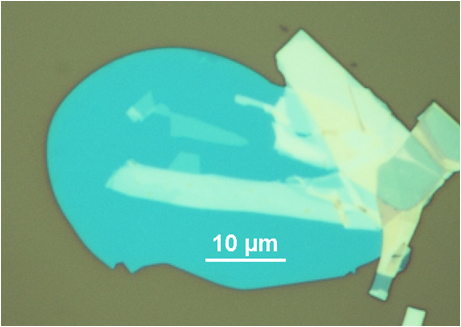
\includegraphics[height=2.5cm,width=3.5cm]{figs/results/hall_bar_doped_channel_doped_contacts/pWSe2_on_hBN_substrate_-6-5_21_no1}
		\label{fig:pWSe2_doped_contacts_and_channel_step1_pt2}
	}
	\qquad
	\subfloat[]{
		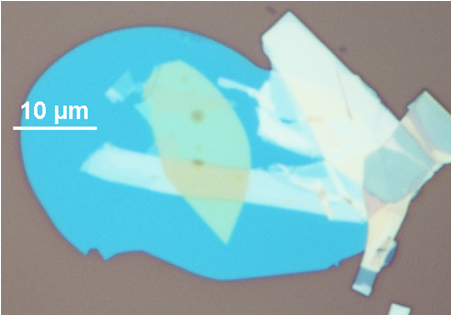
\includegraphics[height=2.5cm,width=3.5cm]{figs/results/hall_bar_doped_channel_doped_contacts/pWSe2_on_hBN_substrate_with_top_hBN_-6-5_21_no1}
		\label{fig:pWSe2_doped_contacts_and_channel_step2_pt2}
	}
	
	\subfloat[]{
		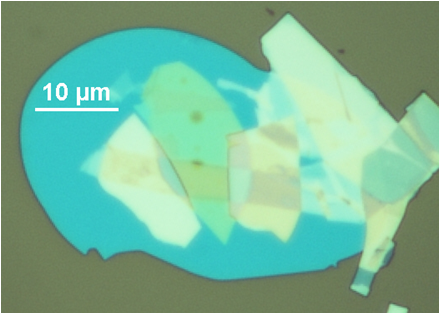
\includegraphics[height=2.5cm,width=3.5cm]{figs/results/hall_bar_doped_channel_doped_contacts/pWSe2_on_hBN_substrate_with_top_hBN_doped_contact_transfer_-6-5_21_no1}
		\label{fig:pWSe2_doped_contacts_and_channel_step3_pt2}
	}
	\qquad
	\subfloat[]{
		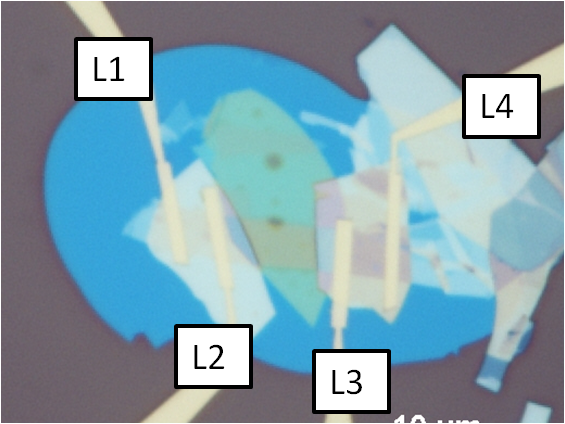
\includegraphics[height=2.5cm,width=3.5cm]{figs/results/hall_bar_doped_channel_doped_contacts/pWSe2_device_with_electrodes_-6-5_21_no1}
		\label{fig:pWSe2_doped_contacts_and_channel_final_device_pt2}
	}
	\caption[\ch{WSe2} device with degenerately doped contacts and lightly doped channel]{\protect\subref{fig:pWSe2_doped_contacts_and_channel_step1_pt2} $0.01\%$ \ch{Nb} doped \ch{WSe2} transferred to \hbn substrate. \protect\subref{fig:pWSe2_doped_contacts_and_channel_step2_pt2} Top \hbn transferred on \ch{WSe2} channel. \protect\subref{fig:pWSe2_doped_contacts_and_channel_step3_pt2} Degenerately doped ($0.5\%$ \ch{Nb} doped \ch{WSe2}) contacts transferred. \protect\subref{fig:pWSe2_doped_contacts_and_channel_final_device_pt2} Device with $0.01\%$ \ch{Nb} doped \ch{WSe2} channel and $0.5\%$ \ch{Nb} doped \ch{WSe2} contacts with electrodes fabricated. Channel dimensions: $L = 9.0\unita{\mu m}$ and $W = 4.02\unita{\mu m}$ with a device thickness of $9\unita{nm}$.}
	\label{fig:doped_contacts_fabrication_steps_pt2}
\end{figure}

\begin{figure}[ht]
	\centering
	\subfloat[]{
		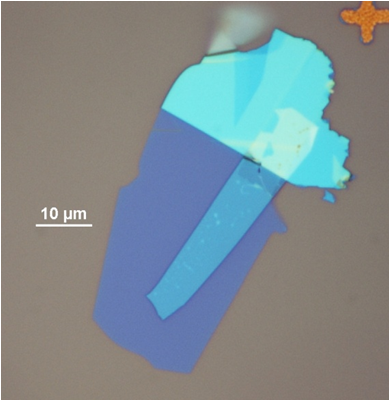
\includegraphics[height=3.75cm,width=3cm]{figs/results/hall_bar_doped_channel_doped_contacts/pWSe2_on_hBN_substrate_5-5_21_no1}
		\label{fig:pWSe2_doped_contacts_and_channel_step1}
	}
	\qquad
	\subfloat[]{
		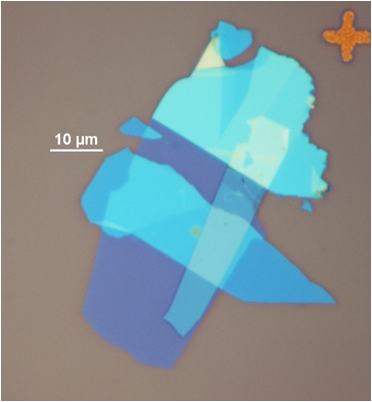
\includegraphics[height=3.75cm,width=3cm]{figs/results/hall_bar_doped_channel_doped_contacts/pWSe2_on_hBN_substrate_with_top_hBN_5-5_21_no1}
		\label{fig:pWSe2_doped_contacts_and_channel_step2}
	}
	\qquad
	\subfloat[]{
		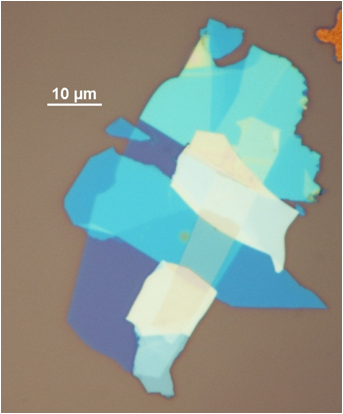
\includegraphics[height=3.75cm,width=3cm]{figs/results/hall_bar_doped_channel_doped_contacts/pWSe2_on_hBN_substrate_with_top_hBN_doped_contact_transfer_5-5_21_no1}
		\label{fig:pWSe2_doped_contacts_and_channel_step3}
	}
	\qquad
	\subfloat[]{
		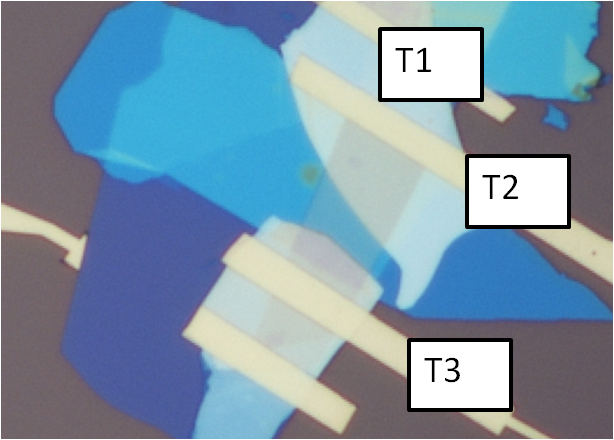
\includegraphics[height=3.75cm,width=3cm]{figs/results/hall_bar_doped_channel_doped_contacts/pWSe2_device_with_electrodes_5-5_21_no1}
		\label{fig:pWSe2_doped_contacts_and_channel_final_device}
	}

	\subfloat[]{
		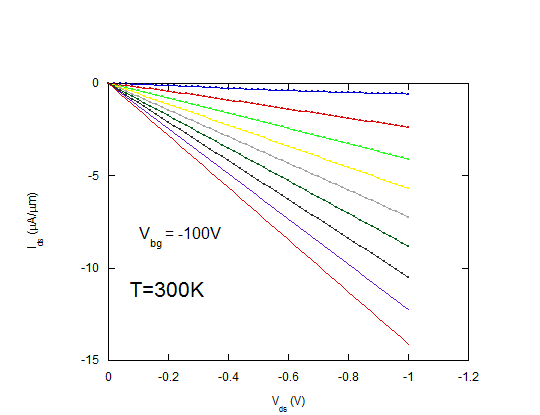
\includegraphics[height=3.5cm,width=4.25cm]{figs/results/hall_bar_doped_channel_doped_contacts/Vds-Id_Vds_1V_-1V-Vbg_-20V_-100V_T2-T3_300K-04_plot_before_anneal_5-5_21_no1}
		\label{fig:5-5_21_no1_pre_anneal_iv_300k}
	}
	\subfloat[]{
		\includegraphics[height=3.5cm,width=4.25cm]{figs/results/hall_bar_doped_channel_doped_contacts/Vds-Id_Vds_1V_-1V-Vbg_-30V_-100V_T2-T3_10K-03_plot_before_anneal_5-5_21_no1}
		\label{fig:5-5_21_no1_pre_anneal_iv_10k}
	}
	\subfloat[]{
		\includegraphics[height=3.5cm,width=4.25cm]{figs/results/hall_bar_doped_channel_doped_contacts/Two_Probe_FE_Mobility_Vs_T_Vds_-1V_-50mV_plot_pre_anneal_5-5_21_no1}
		\label{fig:5-5_21_no1_pre_anneal_mu_fe_vs_temp}
	}
	%\qquad

	\subfloat[]{
		\includegraphics[height=3.5cm,width=4.25cm]{figs/results/hall_bar_doped_channel_doped_contacts/Vds-Id_Vds_1V_-1V-Vbg_-20V_-100V_T2-T3_300K-13_plot_after_anneal_5-5_21_no1}
		\label{fig:5-5_21_no1_post_anneal_iv_300k}
	}
	\subfloat[]{
		\includegraphics[height=3.5cm,width=4.25cm]{figs/results/hall_bar_doped_channel_doped_contacts/Vds-Id_Vds_1V_-1V-Vbg_-30V_-100V_T2-T3_10K-03_plot_after_anneal_5-5_21_no1}
		\label{fig:5-5_21_no1_post_anneal_iv_10k}
	}
	\subfloat[]{
		\includegraphics[height=3.5cm,width=4.25cm]{figs/results/hall_bar_doped_channel_doped_contacts/Two_Probe_FE_Mobility_Vs_T_Vds_-1V_-50mV_plot_post_anneal_5-5_21_no1}
		\label{fig:5-5_21_no1_post_anneal_mu_fe_vs_temp}
	}
	\caption[Degenerately doped contacts and lightly doped channel field-effect mobility]{\protect\subref{fig:pWSe2_doped_contacts_and_channel_step1} $0.01\%$ \ch{Nb} doped \ch{WSe2} transferred to \hbn substrate. \protect\subref{fig:pWSe2_doped_contacts_and_channel_step2} Top \hbn transferred on \ch{WSe2} channel. \protect\subref{fig:pWSe2_doped_contacts_and_channel_step3} Degenerately doped ($0.5\%$ \ch{Nb} doped \ch{WSe2}) contacts transferred. \protect\subref{fig:pWSe2_doped_contacts_and_channel_final_device} Device with $0.01\%$ \ch{Nb} doped \ch{WSe2} channel and $0.5\%$ \ch{Nb} doped \ch{WSe2} contacts with electrodes fabricated. Channel dimensions: $L = 12.9\unita{\mu m}$ and $W = 7.5\unita{\mu m}$ with a device thickness of $5.6\unita{nm}$. \protect\subref{fig:5-5_21_no1_pre_anneal_iv_300k} IV characteristic curves for $V_{bg}$ ranging from $-100\unita{V}$ to $-20\unita{V}$ at $T=300\unita{K}$ before annealing the device. \protect\subref{fig:5-5_21_no1_pre_anneal_iv_10k} IV characteristic curves for $V_{bg}$ ranging from $-100\unita{V}$ to $-20\unita{V}$ at $T=10\unita{K}$ before annealing the device. \protect\subref{fig:5-5_21_no1_pre_anneal_mu_fe_vs_temp} Two-probe field-effect mobility as a function of temperature for $V_{ds}=-50\unita{mV}$ and $V_{ds}=-1\unita{V}$ before annealing the device. \protect\subref{fig:5-5_21_no1_post_anneal_iv_300k} IV characteristic curves for $V_{bg}$ ranging from $-100\unita{V}$ to $-20\unita{V}$ at $T=300\unita{K}$ after annealing the device for 30 minutes at $250^\degree\unita{C}$. \protect\subref{fig:5-5_21_no1_post_anneal_iv_10k} IV characteristic curves for $V_{bg}$ ranging from $-100\unita{V}$ to $-20\unita{V}$ at $T=10\unita{K}$ after annealing the device for 30 minutes at $250^\degree\unita{C}$. \protect\subref{fig:5-5_21_no1_post_anneal_mu_fe_vs_temp} Two-probe field-effect mobility as a function of temperature for $V_{ds}=-50\unita{mV}$ and $V_{ds}=-1\unita{V}$ after annealing the device for 30 minutes at $250^\degree\unita{C}$.}
	\label{fig:two_probe_mu_fe_data}
\end{figure}
\noindent Initially, the IV characteristics for the device in fig.~\subref*{fig:pWSe2_doped_contacts_and_channel_final_device} show ohmic contacts at $T=300\unita{K}$, however, at lower temperatures the contacts are less ohmic. Fig.~\subref*{fig:5-5_21_no1_pre_anneal_iv_300k} shows the linearity expected for various $V_{bg}$ at $T=300\unita{K}$, but one can see that in fig.~\subref*{fig:5-5_21_no1_pre_anneal_iv_10k} there is a deviation in the linearity that is expected of ohmic contacts. This deviation from ohmic contacts at lower temperatures explains the behavior shown in fig.~\subref{fig:5-5_21_no1_pre_anneal_mu_fe_vs_temp} where the field-effect mobility is degraded at lower temperatures ($T<80\unita{K}$). In attempt to improve the contacts at lower temperatures the device was annealed at $250^\degree\unita{C}$ for 30 minutes. The result is improved contacts at lower temperatures, fig.~\subref*{fig:5-5_21_no1_post_anneal_iv_10k} exhibits the linearity expected of ohmic contacts for $T=10\unita{K}$. Annealing removed any residue or absorbant that may have degraded the contact interface. The \acs{PDMS} transfer method, while relatively clean as compared to other available transfer methods, still has the potential to introduce surface residues that can affect the overall device performance, however, it has been shown that while they cannot be elimnated completely, annealing can remove them to some degree and improve device mobility. This change improved the field-effect mobility shown in fig.~\subref*{fig:5-5_21_no1_post_anneal_mu_fe_vs_temp} where the mobility is not degraded for either $V_{ds}$ and the overall values for mobility improved after annealing. The field effect mobility increases with decreasing temperature which is expected behavior. At high temperatures the mobility is largely dominated by phonon scattering which is decreased with temperature. At lower temperatures phonon scattering is decreased compared to room temperature measurements and thus long-range Coulomb scattering and short-range atomic defects play a large role \cite{Ando_RevModPhys1982}. Another possible scattering mechanism is interface scattering or surface roughness scattering. However, the use of a \hbn substrate as opposed to a \ch{Si}/\ch{SiO2} can minimize this scattering mechanism significantly. Channel defects are another source of scattering present in this device. This is largely due to the doping of the \ch{WSe2} channel which introduces impurities that degrades the mobility across all temperatures. \\ \\
\noindent In short, the improved mobility due to the fabrication of a lightly doped channel and using degenerately doped contacts provides stepping-stone toward further refined devices. However, this technique is challenging because as doping decreases the contact resistance, it increases the channel scattering. In order to fully understand the balance and relationship between doping and the trade-off with scattering mechanisms further study of various doping strengths is neeeded. With such devices it will become possible to explore the intrinsic property limits of \acp{TMD}.
 %chap3
	\chapter{Future Works and Conclusion}\label{chap:conclusion}
Certain measurable quantities are valued because of the information they reveal about the geometry of the Fermi surface. Additionally, these quantities are attractive because they depend only on universal constants, experimentally controlled variables, and information about the electronic band structure which is entirely determined by the shape of the Fermi surface \cite{Ashcroft_SolidStatePhysics1978}. These measurable quantities commonly arise in the presence of a strong magnetic field and low temperature system. Determining the Fermi surface geometry provides insight into the transport and scattering properties of the material.

\section{Integer Quantum Hall Effects}\label{sec:IQHE}
In a \ac{2DES} there are a number of interesting phenomena that occurs at low temperatures in the presence of strong magnetic fields. One such effect is the \ac{IQHE}. The \acs{IQHE} was discovered in 1980 by Klitzing \emph{et al.} \cite{Klitzing_PhysRevLett1980}. They showed that under a quantum regime of temperature and magnetic field there is a quantization of the Hall resistance, which deviates from its linearity in the magnetic field seen in the classical Hall effect, displaying plateaus at particular values of the magnetic field where the Hall resistance is given purely in terms of universal constants. In addition, the plateaus observed in the Hall resistance are accompanied by a vanishing longitudinal resistance \cite{Klitzing_PhysRevLett1980,Ando_RevModPhys1982,Goerbig_2009,Hook_Solid1991}.\\ \\

%\subsection{Theoretical Background}\label{subsec:IQHE_theory}
\noindent In order to fully mathematically describe the theory behind the \acs{IQHE} one must first introduce the concept of Landau levels. Here we assume a quantum regime in which there is a low temperature and high magnetic field such that $\hbar\omega\gg k_B T$. The Hamiltonian of a particle in a uniform magnetic field is given by 
\begin{equation}\label{eq:particle_in_b_field}
\hat{H} = \frac{1}{2m}\left(\hat{p}_x+eBy/c\right)^2 + \frac{\hat{p}_y^2}{2m} + \frac{\hat{p}_z}{2m} - \left(\mu/s\right)\hat{s}_z B,
\end{equation}
where $\hat{p}_i$ is the momentum operator in the specified coordinate direction, $B$ is the magnetic field, $e$ is the charge of an electron, $\left(\mu/s\right)\hat{s}_z$ is the intrinsic magnetic moment operator \cite{Landau_Quantum1965}. It is worth noting that the vector potential chosen in eq.~\ref{eq:particle_in_b_field} is known as the Landau gauge, $\vec{A} = \left(-By, 0, 0\right)$, which implies the magnetic field $B$ is directed in the positive $z$-direction \cite{Sakurai_Quantum1994,Landau_Diagmagnetismus1930}. In this case the eigenfunctions of the Hamiltonian must take the form,
\begin{equation}\label{eq:psi_b_field}
\psi\left(\vec{r}\right) = e^{\left(i/\hbar\right)\left(p_x x+p_z z\right)}\chi\left(y\right),
\end{equation} 
where $\chi\left(y\right)$ is defined by solutions to  
\begin{equation}\label{eq:b_field_schrodinger}
	\frac{\partial^2 \chi}{\partial y^2} + \frac{2m}{\hbar^2}\left[E +\left(\mu/s\right)\sigma B - \frac{p_z^2}{2m}-\frac{1}{2}m\left(\frac{e B}{mc}\right)^2\left(y-y_0\right)^2\right]\chi = 0,
\end{equation}
where $y_0 =-c p_x/e B$ and $\omega = \abs{e}B/m c$. Additionally, since the Hamiltonian does not explicitly depend on $x$ and $z$ this implies that both the $x$ and $z$ components of the generalized momentum are conserved. Eq.~\ref{eq:b_field_schrodinger} is formally identical to that of the linear oscillator, thus the expression for the energy levels of a particle in a uniform magnetic field is 
\begin{equation}\label{eq:landau_levels_3D}
	E = \left(n+\frac{1}{2}\right)\frac{\abs{e}\hbar B}{mc} + \frac{p_z^2}{2m} - \left(\mu/s\right)\sigma B,
\end{equation}
where $n$ is any integer \cite{Landau_Quantum1965}. These quantum numbers $n$ specify states known as Landau levels. For the case in which the motion of particles in restricted to a rectangular geometry of $L_x \times L_y$, also let $p_z=0$ as the motion of particles is restricted in this case to only the $x-y$ plane. In this case the energy of each Landau level is given by 
\begin{equation}\label{eq:landau_levels_2D}
	E = \left(n+\frac{1}{2}\right)\frac{\abs{e}\hbar B}{mc} - \left(\mu/s\right)\sigma B.
\end{equation}
Due to the restriction that $\hbar\omega \gg k_B T$, thermal excitations can be neglected because the interval between Landau levels is much greater than thermal excitation energy. As a result, the probability that electrons will be thermally excited to higher energy levels can be neglected. In order to fill higher energy levels the density of states must be increased. When the Landau level is fully occupied from the lowest to the $i\mathrm{th}$ energy level the transverse resistivity becomes
\begin{equation}\label{eq:rho_xy}
	\rho_{xy} = \frac{h}{i e^2},
\end{equation}
where $i$ is any integer corresponding to a specific filled Landau level, $e$ is the charge of an electron, and $h$ is Planck`s constant \cite{Klitzing_PhysRevLett1980,Goerbig_2009}. Eq.~\ref{eq:rho_xy} shows that at critical values of the field, the Hall resistivity (or conductivity) is quantized in units of $h/e^2$ \cite{Kittel_IntroSolidState2005,Hook_Solid1991}. 
\begin{figure}[ht]
	\centering
	\includegraphics[height=5cm,width=5cm]{figs/future/IQHE_data_RHOxy_RHOxx}
	\caption[Example data of the Integer Quantum Hall Effect]{$\rho_{xy}$ as a function of magnetic field $B$ at low temperature ($T=50\unita{mK}$). Figure originally appeared in ref.~\cite{Paalanen_PhysRevB1982}.}
	\label{fig:IQHE_data}
\end{figure}
Fig.~\ref{fig:IQHE_data} demonstrates an example of the quantized nature of the transverse resistivity. The distance between each plateau (step height) is given by $h/e^2$ divided by an integer $i$. These steplike increases with plateaus in the magnetic field region where the longitudinal resistivity $\rho_{xx}$ vanished \cite{Klitzing_RevModPhys1986}. Thus, when $\rho_{xx} = 0$ then $\rho_{xy} = h/i e^2$ and is at a plateau. Note that the temperatures needed to observe the \acs{IQHE} ($\lesssim 4\unita{K}$) is a likely reason why it was not discovered until 1980. It is also important to note that the value of resistivity only depends on fundamental constants of physics and can be used as a primary resistance standard known as the von Klitzing constant, $R_{\mathrm{K}-90} = 25812.807\unita{\Omega}$ \cite{Klitzing_PhysRevLett1980,Aoki_PhysRevLett1986,Bliek_Met1988}. Observation of the \acs{IQHE} confirms the high-quality nature of the device in question as it is necessary to obtain high mobilities at very low temperatures. Furthermore, this would offer a more complete picture of the quantum structure of under the high-field limit and allow for the measurement of further quantum properties that reveal important information about the underlying structure of the device.%\\ \\ 

\section{Shubnikov-de Haas Oscillations}\label{sec:qm_oscillations}
There are several techniques and measurements that can determine the geometry of the Fermi surface, many of these are closely related to one another and are based on the same underlying mechanism. One such effect is the \acs{SdH} effect \cite{Shubnikov_Leiden1930}. The \acs{SdH} effect is an oscillatory dependence of the resistivity on the magnetic field, there it is related to the \ac{QHE} \cite{Soule_PhysRev1964}. This effect is produced by the oscillation of the density of states at the Fermi level which is caused by the quantization of electron energy levels in the presence of a magnetic field (see sec.~\ref{sec:IQHE}, Landau levels) \cite{Peierls_ZPhys1933,Landau_RoyalSoc1939}. The oscillations occur with a periodicity of $B^{-1}$ \cite{Shoenberg_Magnet1984}.\\ \\

\noindent \acs{SdH} oscillations can provide a wealth of information about the effective \acs{2DEG} (\acs{2DHG}). For example, one can extract the carrier lifetimes, effective cyclotron mass, information about the Fermi surface \cite{Li_NatureNano2015}. In order to observe the \acs{QHE} and therefore observe \acs{SdH} oscillations, high device mobility is required \cite{Das_Wiley1996,Tsukazak_Science2007}. Recently the Cui \emph{et al.} observed the first \acs{SdH} oscillations in \ch{MoS2}, Li \emph{et al.} and Gillgren \emph{et al.} observed this same effect in black phosphorus (and phosphorene) \cite{Cui_NatureNano2015,Li_NatureNano2015,Gillgren_2DMat2015}. Cui \emph{et al.} were able to determine geometry of the Fermi surface from the oscillation frequency and prove the two-dimensional nature of their system. Furthermore, from the analysis of the oscillation amplitude the cyclotron effective masses of both electrons and holes could be determined. From this method the carrier lifetime could also be determined, they reported lifetimes of $\tau = 0.11\unita{ps}$ and $\tau = 0.12\unita{ps}$ for holes and electrons, respectively \cite{Li_NatureNano2015,Shoenberg_Magnet1984}. Cui \emph{et al.} was able to provide insight about the quantum lifetimes and the underlying interactions between short-range and long-range scattering limits \cite{Cui_NatureNano2015}. The results provide promise that with the implementations of improvements in contact resistance reduction and further mobility enhancement that the world of \acp{TMD} is closer to the routine study of novel quantum physics in \td systems. 

\section{Performance Limits in \acp{TMD}}\label{sec:performance_limits}
The ultimate performance limit of \acp{TMD} is of interest, especially at room temperature as this is most relevant to device applications. 
%Again, one of the main obstacles that hinders from gaining definitive insight in this area is contact resistance. 
First principles calculations show mobility in monolayer \ch{MoS2} to be $\sim 320-410\cmvs$ at room temperature depending on initial parameters \cite{Li_PhysRevB2013,Kaasbjerg_PhysRevB2012}. Previously the experimental values reported differed by an order of magnitude compared to first principles calculations, however, the improvements made in the area of reducing contact resistance has improved mobility measurements \cite{Radisavljevic_NatureNano2011,Kappera_APLmat2014}. Experimentally, room temperature mobility measurements of both $p$ and $n$ type semiconductors still lag behind the theoretical calculations. For example, \ch{WSe2} room temperature mobilities have been reported as $\sim 200\cmvs$ with perfect subthreshold swings of $\sim 60\unita{mV}/\unita{dec}$, a $I_\mathrm{on}/I_\mathrm{off}$ of $> 10^6$ at room temperature (others have shown $I_\mathrm{on}/I_\mathrm{off}$ of $> 10^7$ in \ch{WSe2} and \ch{MoS2}), and high $I_\mathrm{on} = 205\unita{\mu A}/\unita{\mu m}$ \cite{Fang_NanoLett2012,Liu_NanoLett2013,Kappera_NatureMat2014,Das_NanoLett2014}.  To further improve the mobilities measured at room temperature a further understanding of scattering mechanisms is needed. At room temperature phonon scattering limits the mobility, the mobility can be enhanced by doping, however, this introduces impurities and can have an adverse effect on the mobility. Understanding the performance limit at room temperature in monolayers is key to applications in which several \acp{TMD} are already being implemented, such as \ac{TFT} and components of \acp{IC} like analog amplifiers, digital inverters, and memory transistors \cite{Bhimanapati_ACSnano2015}.

\section{Conclusion}\label{sec:conclusion}
Overall, \acp{TMD} offer a wealth of opportunities in applications. In order to realize these proposed applications several challenges must be overcome, namely achieving low-resistance contacts and high mobility at room temperature. The approach of using degenerately doped contacts and \hbn encapsulated devices to lower the \acs{SBH} and promote increased mobility has shown potential. In addition, the increased mobility that the success of this method would allow one to study quantum transport properties which will reveal many fundamental properties, such as quantum scattering times and effective masses.  %!!!!!!!!!!!!!uncomment


%---- References and bib data
	%\addcontentsline{toc}{section}{References}
	\bibliographystyle{unsrt}
	\bibliography{refs/database}


	\begin{appendices} 
		\begin{acronym}
	\acro{AFM}{atomic force microscopy}
	\acro{Au}[\ch{Au}]{gold}
	\acro{DI}{deionized water}
	\acro{DFT}{density functional theory}
	\acro{FET}{field effect transistor}
	\acro{hBN}[$h$-\ch{BN}]{boron nitride}
	\acro{IC}{integrated circuit}
	\acro{IPA}{isopropanol}
	\acro{MEK}{methyl ethyl ketone}
	\acro{MFM}{magnetic force microscopy}
	\acro{MIBK}{methyl isobutyl ketone}
	\acro{Mo}[\ch{Mo}]{molybdenum}
	\acro{MoS2}[\ch{MoS2}]{molybdenum disulfide}
	\acro{MOSFET}{metal-oxide-semiconductor field-effect transistor}
	\acro{N2}[\ch{N2}]{nitrogen}
	\acro{Nb}[\ch{Nb}]{niobium}
	\acro{Ni}[\ch{Ni}]{nickel}
	\acro{PC}{polycarbonate}
	\acro{PDMS}{polydimethylsiloxane}
	\acro{PPMS}{physical property measurement system}
	\acro{Re}[\ch{Re}]{rhenium}
	\acro{S}[\ch{S}]{sulfur}
	\acro{Se}[\ch{Se}]{selenium}
	\acro{SEM}{scanning electron microscope}
	\acro{SiO2}[\ch{SiO2}]{silicon dioxide}	
	\acro{STM}{scanning tunneling microscopy}
	\acro{Te}[\ch{Te}]{tellurium}
	\acro{TEM}{transmission electron microscopy}
	\acro{TMD}{transition metal dichalcogenides}
	\acro{V}[\ch{V}]{vanadium}
	\acro{W}[\ch{W}]{tungsten}
	\acro{WS2}[\ch{WS2}]{tungsten disulfide}
	\acro{WSe2}[\ch{WSe2}]{tungsten diselenide}
\end{acronym} 
	\end{appendices} 
	\newpage
\begin{center}
{\bf ACKNOWLEDGEMENTS}
\end{center}

I would like to acknowledge the continued guidance, help, and support from my advisor Dr. Zhixian Zhou. I am also grateful to Hsun Jen (Ben) Chuang, Bhim Chamlagain, Meeghage Madusanka Perera, Arthur Bowman III, Upendra Rijal, and Sagar Paudel for their advice and cooperation. Finally, I would like to thank the committee members Dr. Jian Huang, Dr. Mark Ming-Cheng Cheng and Dr. Ashis Mukhopadhyay for their valuable time. %!!!!!!!!!!!!!uncomment

\end{document}
